\sisetup{locale = DE} 
%%%%%%%%%%%%%%%%%%%%%%%%%%%%%%%%%%%%%%%%%%%%%%%%%%%%%%%%%%%%%%%%%%%%%%%%%%%%%%%%%%%%%%%%%%%%%%
%
%   GERMAN
%
%%%%%%%%%%%%%%%%%%%%%%%%%%%%%%%%%%%%%%%%%%%%%%%%%%%%%%%%%%%%%%%%%%%%%%%%%%%%%%%%%%%%%%%%%%%%%%
\usetikzlibrary {arrows.meta}
\usepackage{stix}
\date{\dateMC}
\title{\textbf{\rmfamily Einführungsvortrag}}
\subtitle{\horrorfont Das Standardmodell der Teilchenphysik und der LHCb Detektor}
\author[~\WorkGroup~]{{\WorkGroup}}
\institute[\WorkGroup]{ \University}

%%%%%%%%%%%%%%%%%%%%%%%%%%%%%%%%%%%%%%%%%%%%%%%%%%%%%%%%%%%%%%%%%%%%%%%%%%%%%%%%%%%%%%%%%%%%%%
%   Options for the footline
%%%%%%%%%%%%%%%%%%%%%%%%%%%%%%%%%%%%%%%%%%%%%%%%%%%%%%%%%%%%%%%%%%%%%%%%%%%%%%%%%%%%%%%%%%%%%%
\setbeamertemplate{footline}
{
\leavevmode%
\hbox{%
\begin{beamercolorbox}[wd=0.5\paperwidth,ht=2.25ex,dp=1ex,center]{author in foot}%
\usebeamerfont{author in foot} \parbox{0.5\paperwidth}{\insertsubsection{}}
\end{beamercolorbox}%
\begin{beamercolorbox}[wd=0.11\paperwidth,ht=2.25ex,dp=1ex,center]{title in head/foot}%
\usebeamerfont{title in head/foot}
\end{beamercolorbox}%
\begin{beamercolorbox}[wd=0.385\paperwidth,ht=2.25ex,dp=1ex,right]{date in head/foot}%
\usebeamerfont{date in head/foot}\insertsection{}\hfill
|~Folie \insertframenumber{} \hspace*{2ex}%/ \inserttotalframenumber\hspace*{2ex}
\end{beamercolorbox}}%
\vskip0pt%
}


%%%%%%%%%%%%%%%%%%%%%%%%%%%%%%%%%%%%%%%%%%%%%%%%%%%%%%%%%%%%%%%%%%%%%%%%%%%%%%%%%%%%%%%%%%%%%%
\newcommand{\midlabelline}[3]{
   \node (midlabel) at ($ (#1)!.5!(#2) $) {#3};
   \draw[<-] (#1) --  (midlabel);
   \draw[->] (midlabel) -- (#2);
}
\begin{document}\selectlanguage{ngerman}



\begin{frame}[plain]
\begin{center}
    \begin{tabular}{ccc}
 \parbox{0.33\textwidth}{\LogoInsitute}    &
 ~~~~\parbox{0.33\textwidth}{
\includegraphics[height=1cm]{Logos And Group/LHCb_Logo.png}}   &  \parbox{0.33\textwidth}{\LogoUniversity}\\
\end{tabular}
\end{center}

\maketitle
\end{frame}

%%%%%%%%%%%%%%%%%%%%%%%%%%%%%%%%%%%%%%%%%%%%%%%%%%%%%%%%%%%%%%%%%%%%%%%%%%%%%%%%%%%%%%%%%%%%%%
% \begin{frame}{Motivation}
% We start with the scale picture, using practical questions to get to microscopic regime 
%     - "What is it made of and how do we know it?"   %%% Hier ist darauf zu achten, dass die Messaperaturen besprochen werden: Auge, Licht, Mikroskop ... etc. Bereitet Grundlegendes Verständig für Detektoren vor
% \end{frame}
% \begin{frame}{How do we measure matter?}
%     We motivate the students to answer the question themselves
% \end{frame}
%%%%%%%%%%%%%%%%%%%%%%%%%%%%%%%%%%%%%%%%%%%%%%%%%%%%%%%%%%%%%%%%%%%%%%%%%%%%%%%%%%%%%%%%%%%%%%
\section{Einführung in die Teilchenphysik}
%%%%%%%%%%%%%%%%%%%%%%%%%%%%%%%%%%%%%%%%%%%%%%%%%%%%%%%%%%%%%%%%%%%%%%%%%%%%%%%%%%%%%%%%%%%%%%
\begin{frame}[plain]
   \begin{center} 
  \huge{  \ding{182} }\\
   \Large{Einführung in die Teilchenphysik}
\end{center}
\end{frame}
%%%%%%%%%%%%%%%%%%%%%%%%%%%%%%%%%%%%%%%%%%%%%%%%%%%%%%%%%%%%%%%%%%%%%%%%%%%%%%%%%%%%%%%%%%%%%%
\begin{frame}[t]{Und was ist eigentlich im Nukleus?}

    \begin{minipage}{\linewidth}
        \begin{minipage}{0.33\linewidth}
             \qquad Atom 
        \end{minipage}     
        \begin{minipage}{0.4\linewidth}
             \quad Atomkern 
        \end{minipage}    
        \begin{minipage}{0.24\linewidth}
            \quad\textbf{Quarks}
        \end{minipage}    
    \end{minipage} \vspace{0.5cm}
    
     \begin{minipage}{0.99\linewidth}
        \begin{figure}
            \centering
            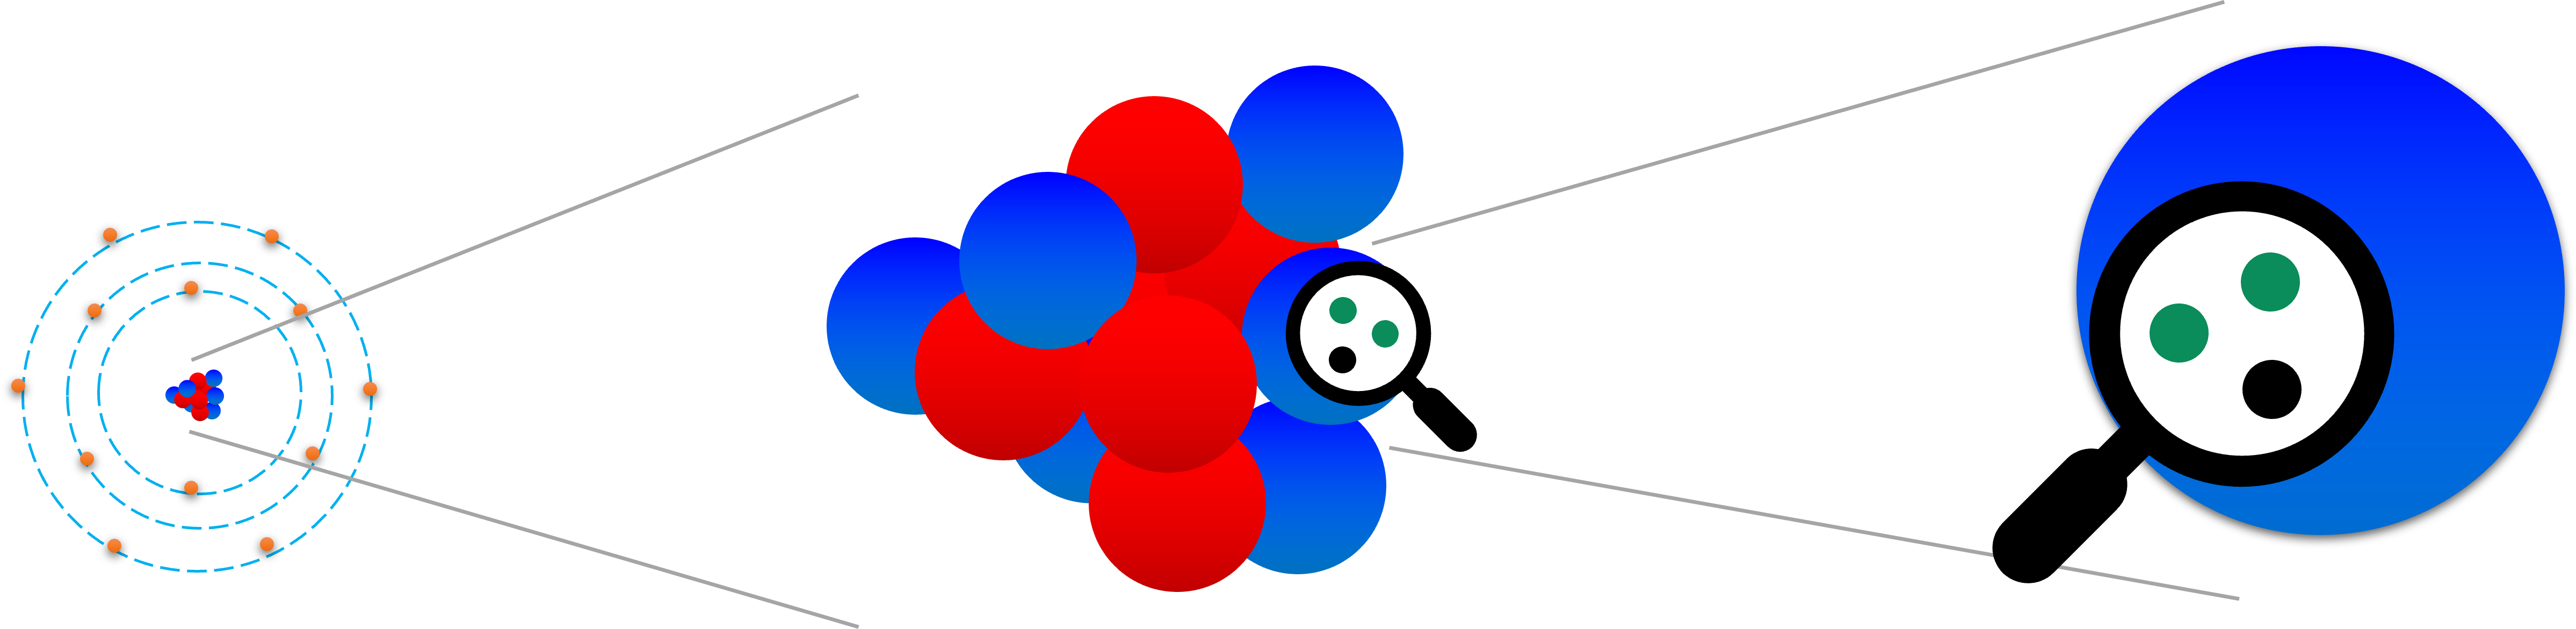
\includegraphics[width=\textwidth]{Figures Introductory Lecture/Standard Model/Scale_Atom_Quark_noText_2.png}
           % \caption{Caption}
            \label{fig:scale_atom_qaurk}
        \end{figure}
     \end{minipage}  
     \vspace{-15cm}
    \begin{minipage}{\linewidth}
        \begin{minipage}{0.33\linewidth}
            \qquad \Large $10^{-10}$\,m
        \end{minipage}     
        \begin{minipage}{0.33\linewidth}
             \quad \Large $10^{-15}$\,m
        \end{minipage}    
        \begin{minipage}{0.29\linewidth}
            \quad \Large $\leq10^{-18}$\,m
        \end{minipage}    
    \end{minipage}

\end{frame}
%%%%%%%%%%%%%%%%%%%%%%%%%%%%%%%%%%%%%%%%%%%%%%%%%%%%%%%%%%%%%%%%%%%%%%%%%%%%%%%%%%%%%%%%%%%%%%
%\begin{frame}{Quark im Nukleus?!}
%    Bild von dem Milchprodukt in verschiedenen Geschmäckern
%\end{frame}
%%%%%%%%%%%%%%%%%%%%%%%%%%%%%%%%%%%%%%%%%%%%%%%%%%%%%%%%%%%%%%%%%%%%%%%%%%%%%%%%%%%%%%%%%%%%%%
%\begin{frame}<presentation:0>{Theorie/Quarks - Hannah}
%    Here should be the typical scale picture. We start with an atom and move to quarks via nuclei and protons/neutrons. (Magnefying glass on proton/neutron and show the quarks) 
    
%    Goal: Students know that the proton consists of three subparticles. Two of these are identical (AAB (uud) and BBA (ddu)) 
%\end{frame}


%\begin{frame}<presentation:0>{Weiteres - Hannah}
%    Eventuell vergleich von theoretischer und experimentalphysik ziehen und für das Forschungsgebiet um die Starke Wechselwirkung ableiteten, dass beide Hand in Hand gehen müssen ("Blackbox").
%\end{frame}
%%%%%%%%%%%%%%%%%%%%%%%%%%%%%%%%%%%%%%%%%%%%%%%%%%%%%%%%%%%%%%%%%%%%%%%%%%%%%%%%%%%%%%%%%%%%%%

\begin{frame}{Quarks - Was sind das?}

    \begin{minipage}[t]{\linewidth}\raggedleft
           Welche Ladung hat ein \textcolor{red}{\textbf{Neutron}}/\textcolor{blue}{\textbf{Proton}}? \\
           Welche Ladung müssen die \textcolor{darkgreen}{\textbf{Q}}\textbf{u}\textcolor{darkgreen}{\textbf{a}}\textbf{r}\textcolor{darkgreen}{\textbf{k}}\textbf{s} haben?
    \end{minipage}%
    \vspace{-0.6cm}
    \begin{minipage}{\linewidth}\raggedright
        \begin{figure}[htb]
            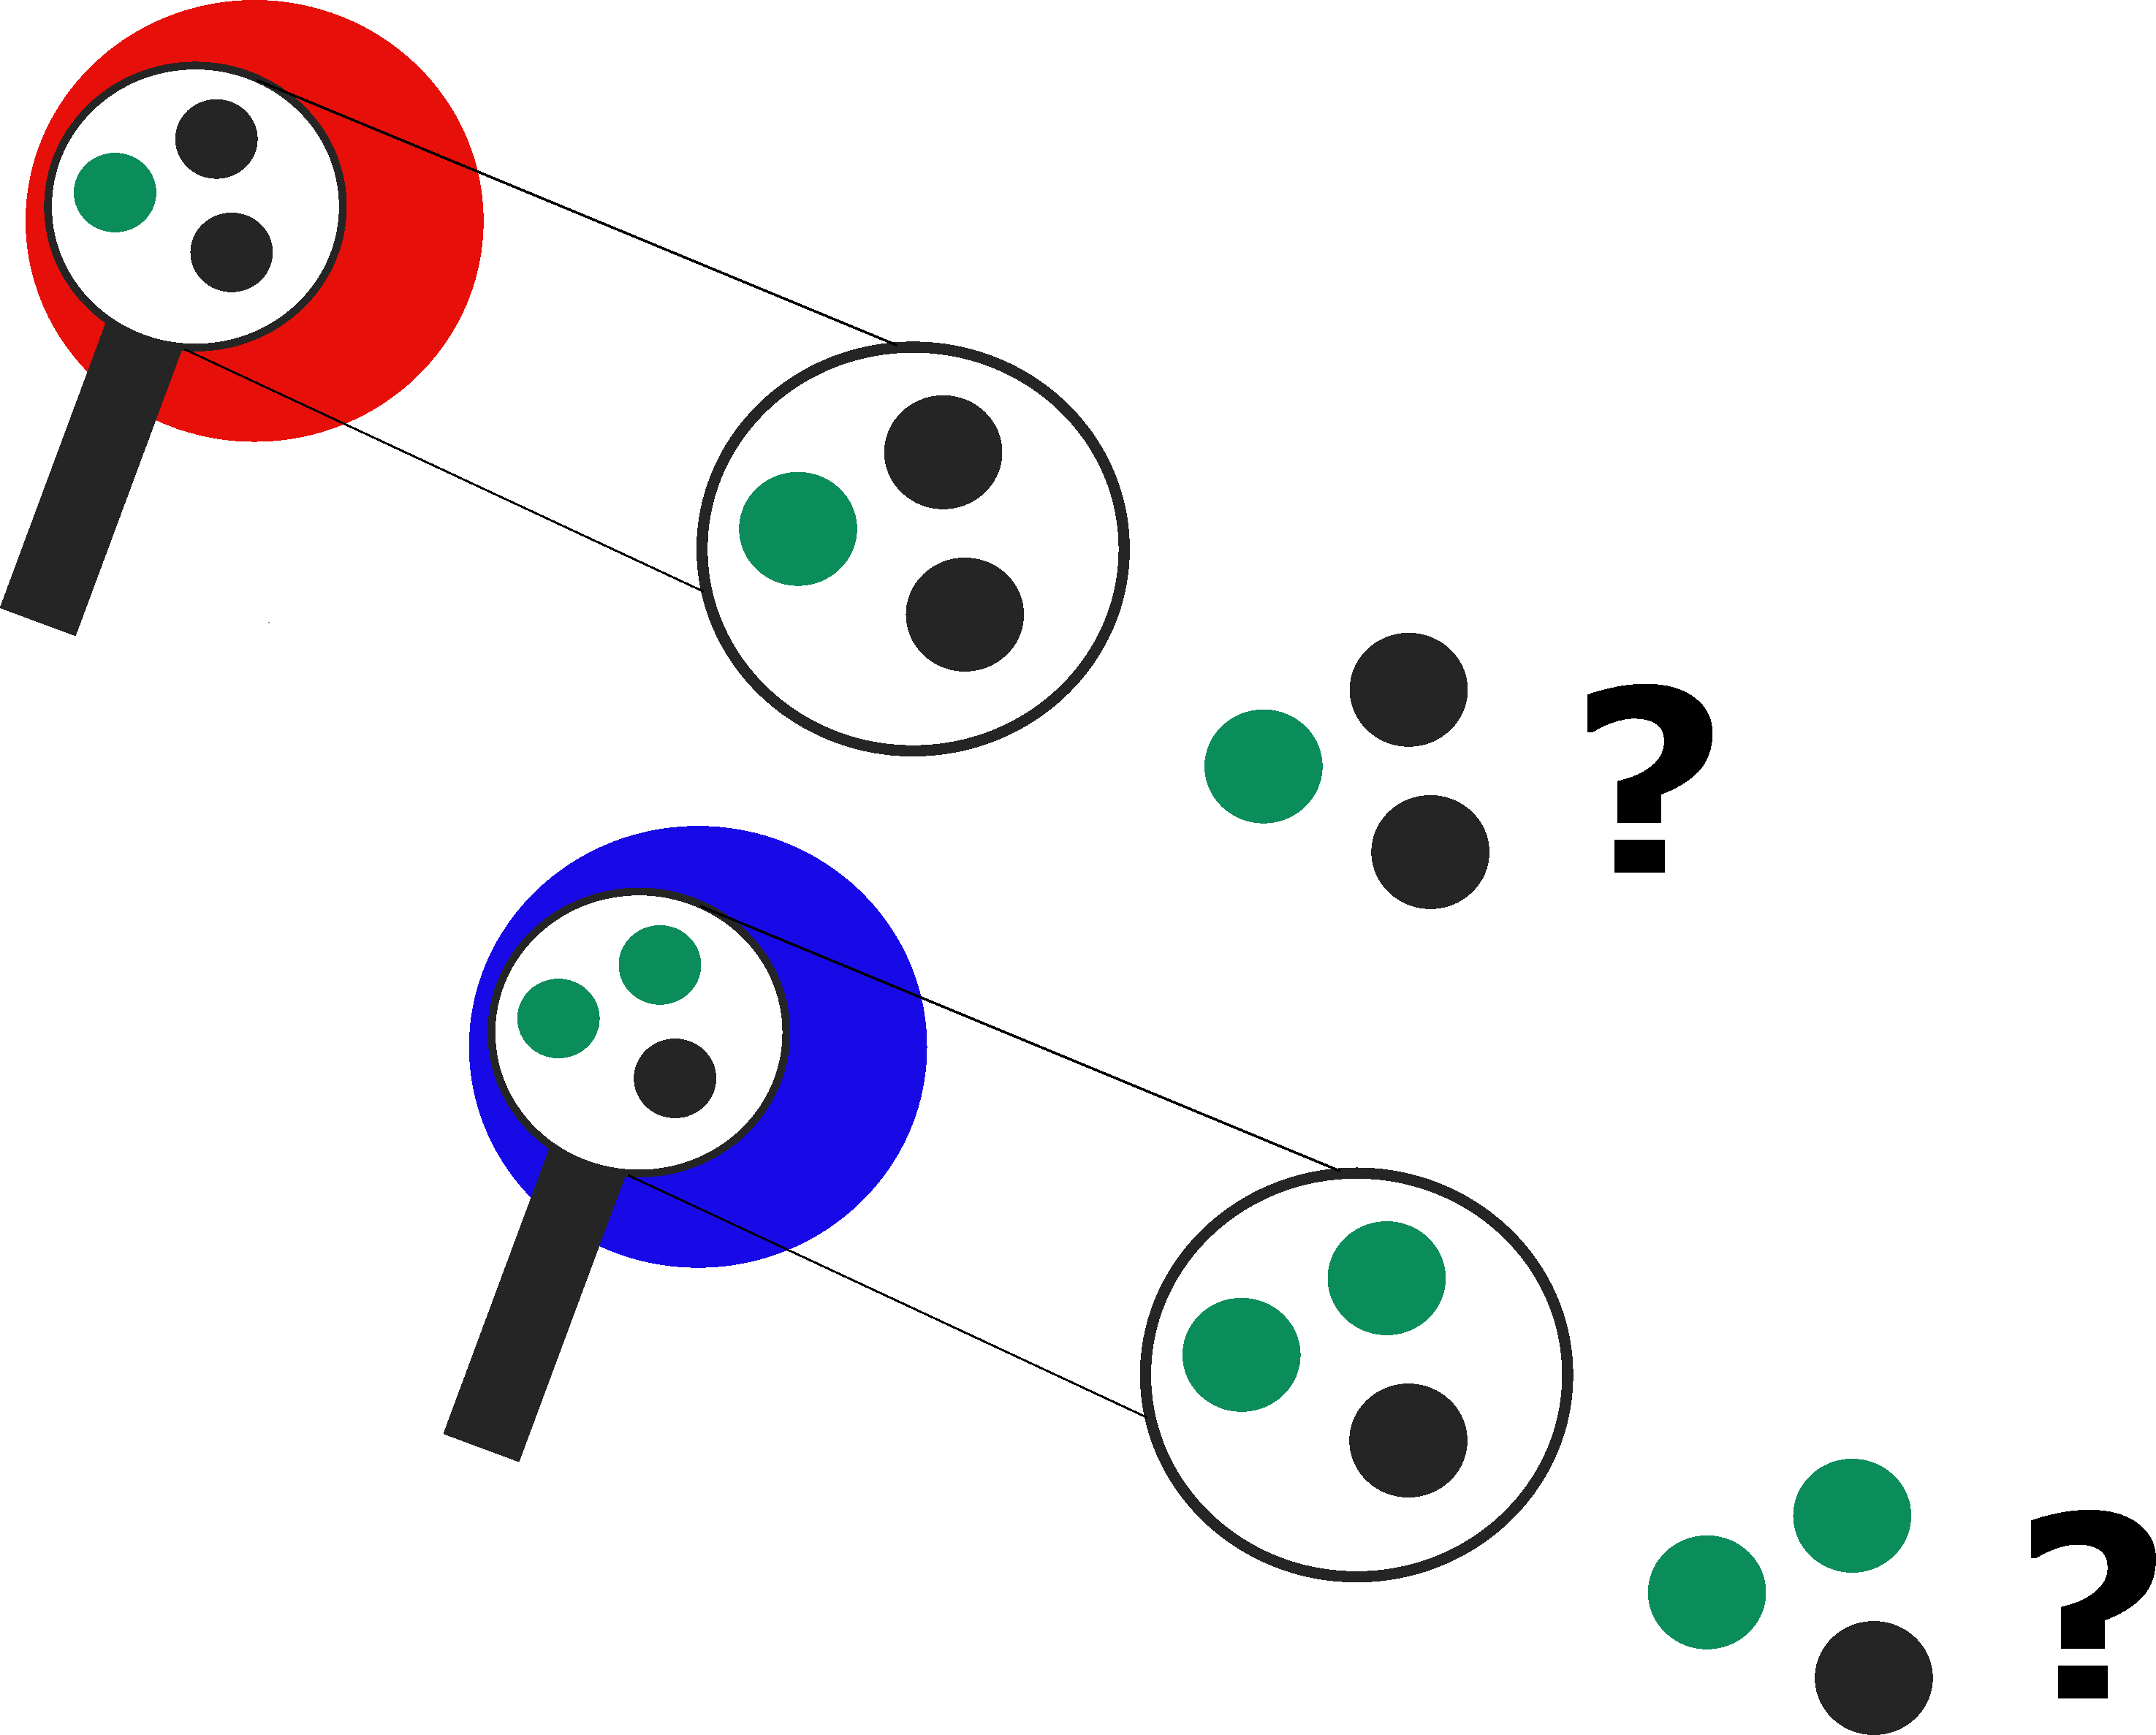
\includegraphics[width=0.79\textwidth]{Figures Introductory Lecture/Standard Model/Quarks.png}
            %\caption{}
            \label{fig:quarks}
        \end{figure}            
    \end{minipage}
    
\end{frame}
%%%%%%%%%%%%%%%%%%%%%%%%%%%%%%%%%%%%%%%%%%%%%%%%%%%%%%%%%%%%%%%%%%%%%%%%%%%%%%%%%%%%%%%%%%%%%%

%\begin{frame}{Quarks - Was ist das?}
%Here we introduce the quarks. We know the proton/neutron has 3 subparticles. Students should know the electric charge of proton/neutron. How can we combine 3 particles to form an electric positive and neutral particle. 

%Goal: quark composition of proton/neutron. No need to mention up and down yet
%\end{frame}
%%%%%%%%%%%%%%%%%%%%%%%%%%%%%%%%%%%%%%%%%%%%%%%%%%%%%%%%%%%%%%%%%%%%%%%%%%%%%%%%%%%%%%%%%%%%%%
\begin{frame}{Wie werden Quarks zusammengehalten?}  
    \begin{figure}[htb]
        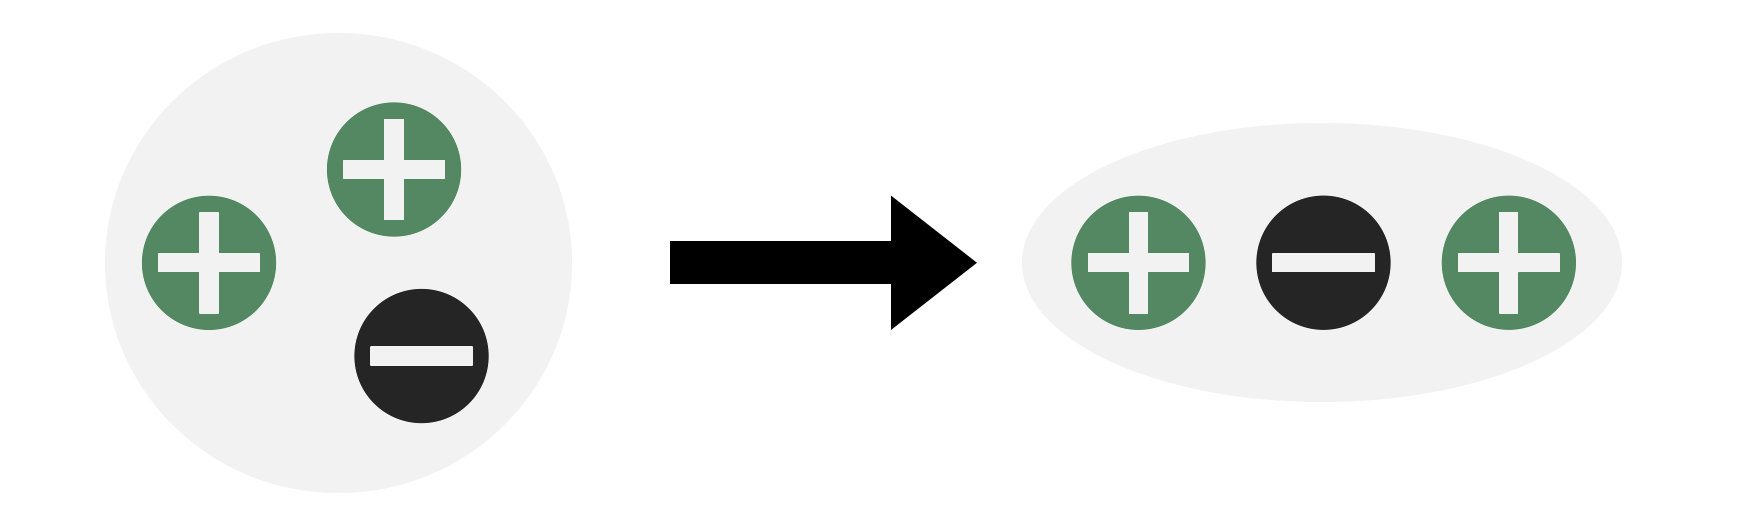
\includegraphics[width=1\textwidth]{Figures Introductory Lecture/Standard Model/StrongForce_EM.png}
        %\caption{}
        \label{fig:strong_force_1}
    \end{figure} \\
    \Large \begin{center}
        Die Elektromagnetische Kraft \emph{könnte} Quarks binden!
    \end{center}
\end{frame}
%%%%%%%%%%%%%%%%%%%%%%%%%%%%%%%%%%%%%%%%%%%%%%%%%%%%%%%%%%%%%%%%%%%%%%%%%%%%%%%%%%%%%%%%%%%%%%
% Zweiter Satz als Gegenfrage .. Aber warum halten Protonen zusammen? 
\begin{frame}{Kräfte in Atomkernen}
...aber warum halten dann \emph{Atomkerne} zusammen?!\\ \, \hspace{2cm} \ding{43} \textcolor{blue}{\textbf{Protonen}} stoßen sich elektromagnetisch ab!

    \begin{figure}[htb]
        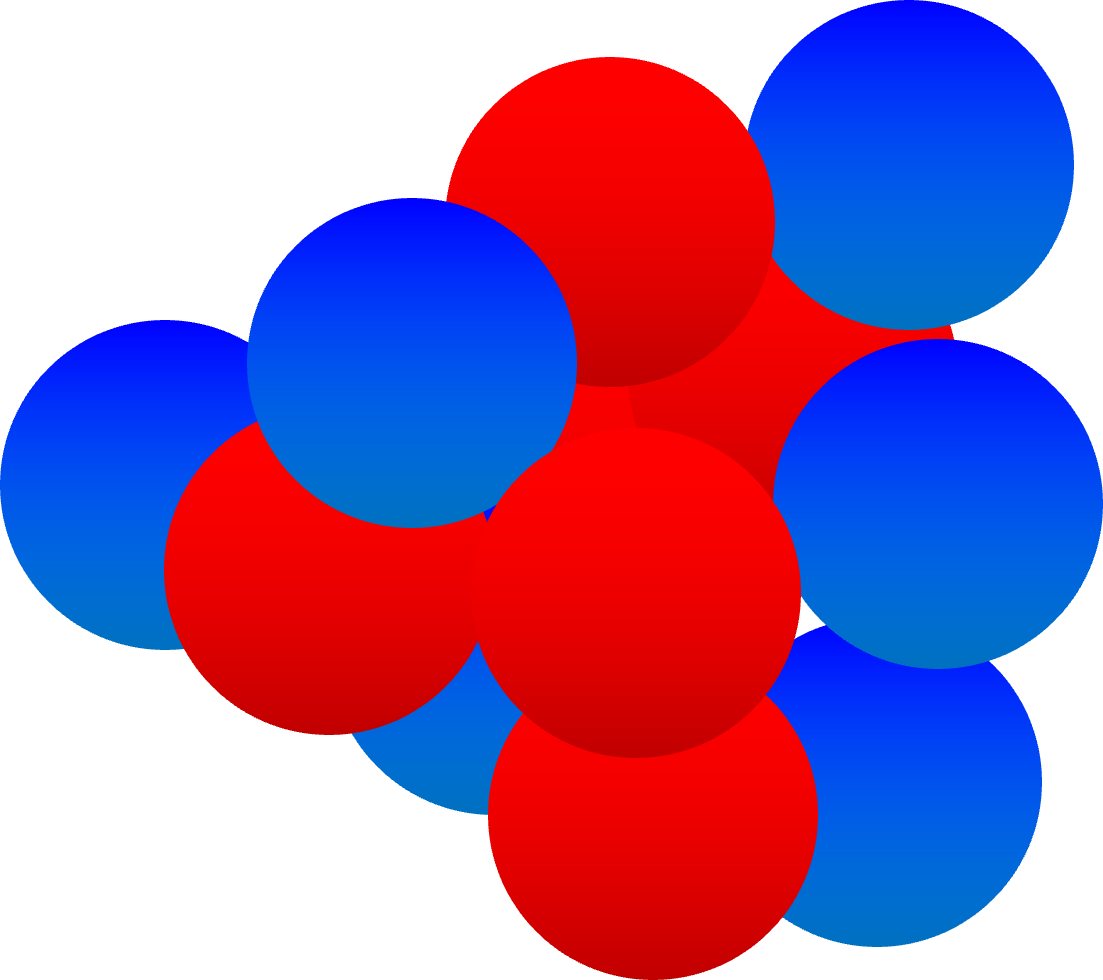
\includegraphics[width=0.3\textwidth]{Figures Introductory Lecture/Standard Model/Nukleus.png}
        %\caption{}
        \label{fig:strong_force_2}
    \end{figure}\\ \pause
    \ding{43} Es gibt weitere Kraft, die Atomkerne bindet\\ 
    \vspace{0.5cm}\begin{center}
    \Large{Die \textbf{starke Kraft}}
    \end{center}
\end{frame}
%%%%%%%%%%%%%%%%%%%%%%%%%%%%%%%%%%%%%%%%%%%%%%%%%%%%%%%%%%%%%%%%%%%%%%%%%%%%%%%%%%%%%%%%%%%%%%
% Protonen -> B
\begin{frame}{Fragestunde Protonen}
\begin{center} \Large
        ...aber, \\ wie können wir feststellen, ob Protonen nun von der\\ starken oder elektromagnetischen Kraft \\zusammengehalten werden? 
\end{center}

\end{frame}
%%%%%%%%%%%%%%%%%%%%%%%%%%%%%%%%%%%%%%%%%%%%%%%%%%%%%%%%%%%%%%%%%%%%%%%%%%%%%%%%%%%%%%%%%%%%%%
% Graue Kreise dunkler machen -> keine chance auf dem Beamer
% Masse weg
% u und d an quarks dranschreiben, oder im Text einbauen
\begin{frame}{Andere Quarkkombinationen}
Tatsächlich finden wir Teilchen, die aus drei  up-Quarks/drei down-Quarks bestehen!
    \begin{figure}[htb]
        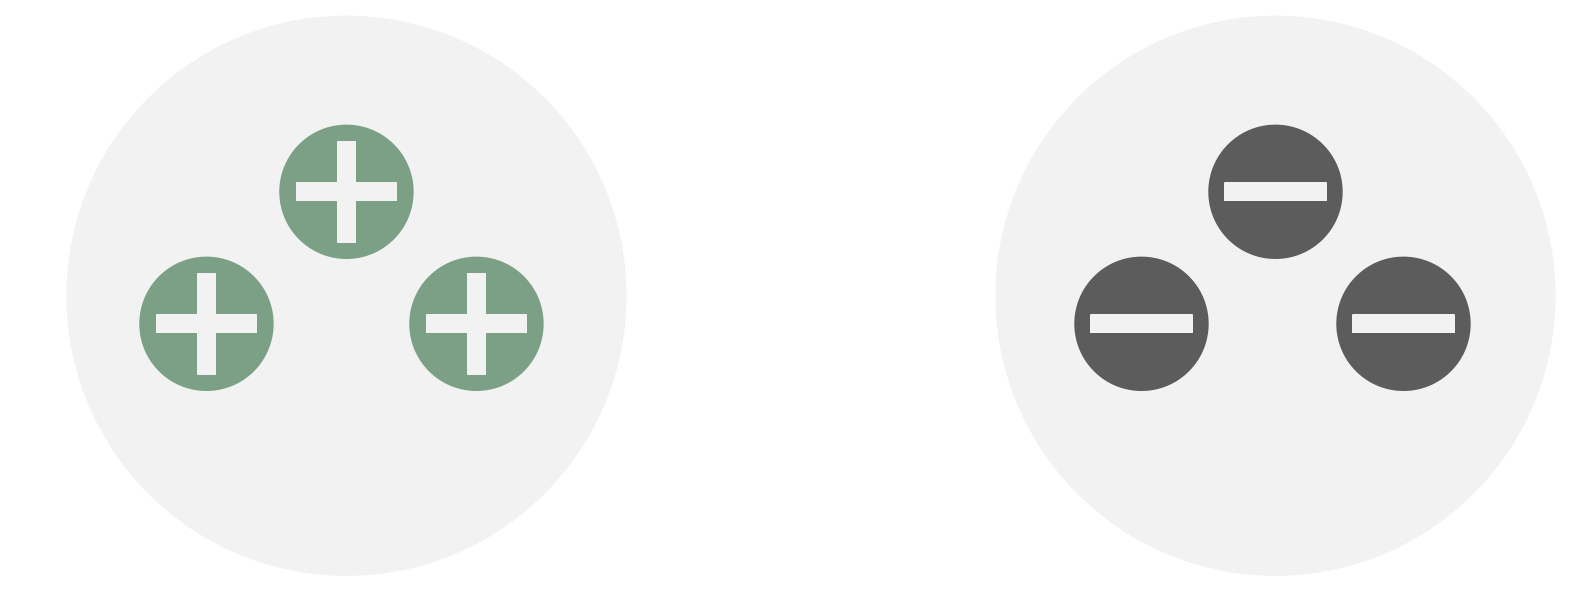
\includegraphics[width=0.6\textwidth]{Figures Introductory Lecture/Standard Model/DeltaBaryons.png}
        %\caption{}
        \label{fig:strong_force_2}
    \end{figure}\pause
    $\hspace{3cm}\rightarrow \Delta^{++}$\hspace{3cm} $\rightarrow \Delta^{-}$\\ \vspace{0.5cm}
    \ding{43} Die \textbf{starke Kraft} muss für die Bindung verantwortlich sein!
    % only speakting about strong force, not SM here.
\end{frame}
%%%%%%%%%%%%%%%%%%%%%%%%%%%%%%%%%%%%%%%%%%%%%%%%%%%%%%%%%%%%%%%%%%%%%%%%%%%%%%%%%%%%%%%%%%%%%%
\begin{frame}{Unterschiede der Kräfte}
Wie unterscheiden sich die elektromagnetische und die starke Kraft?
\pause
\begin{itemize}
    % Die EM Kraft ist spürbar!
    \item Wir spüren die starke Kraft  im Alltag nicht
    \item Die starke Kraft wirkt anziehend auf elektrisch neutrale \& geladene Teilchen
    \item ... \pause
    \item[\ding{43}] Wir verstehen die elektromagnetische Kraft, bei der starken Kraft tun wir uns schwerer!
    % Fragen ob den Leuten noch was einfällt...
\end{itemize}
\end{frame}
%%%%%%%%%%%%%%%%%%%%%%%%%%%%%%%%%%%%%%%%%%%%%%%%%%%%%%%%%%%%%%%%%%%%%%%%%%%%%%%%%%%%%%%%%%%%%%
% die auf sie wirkt...
% Quarks müssen eine weitere Ladung haben -> Farbladung
% Wir messen die Farbladung nicht
\begin{frame}{Die Eigenschaften der starken Wechselwirkung} 
Für die \textbf{starke Kraft} existiert eine \textbf{Ladung}, auf die sie wirkt! \\ \pause
\begin{itemize}
\begin{itemize}
    \item [\ding{220}] Quarks müssen eine sog. \textbf{Farbladung} besitzen\\
    \item[] Teilchen, die wir beobachten, sind aber farblos! \\
    \end{itemize}
   \item[] \textbf{Veranschaulichung:}
\end{itemize} \vspace{-0.5cm}
    \begin{figure}[htb]                                                 
    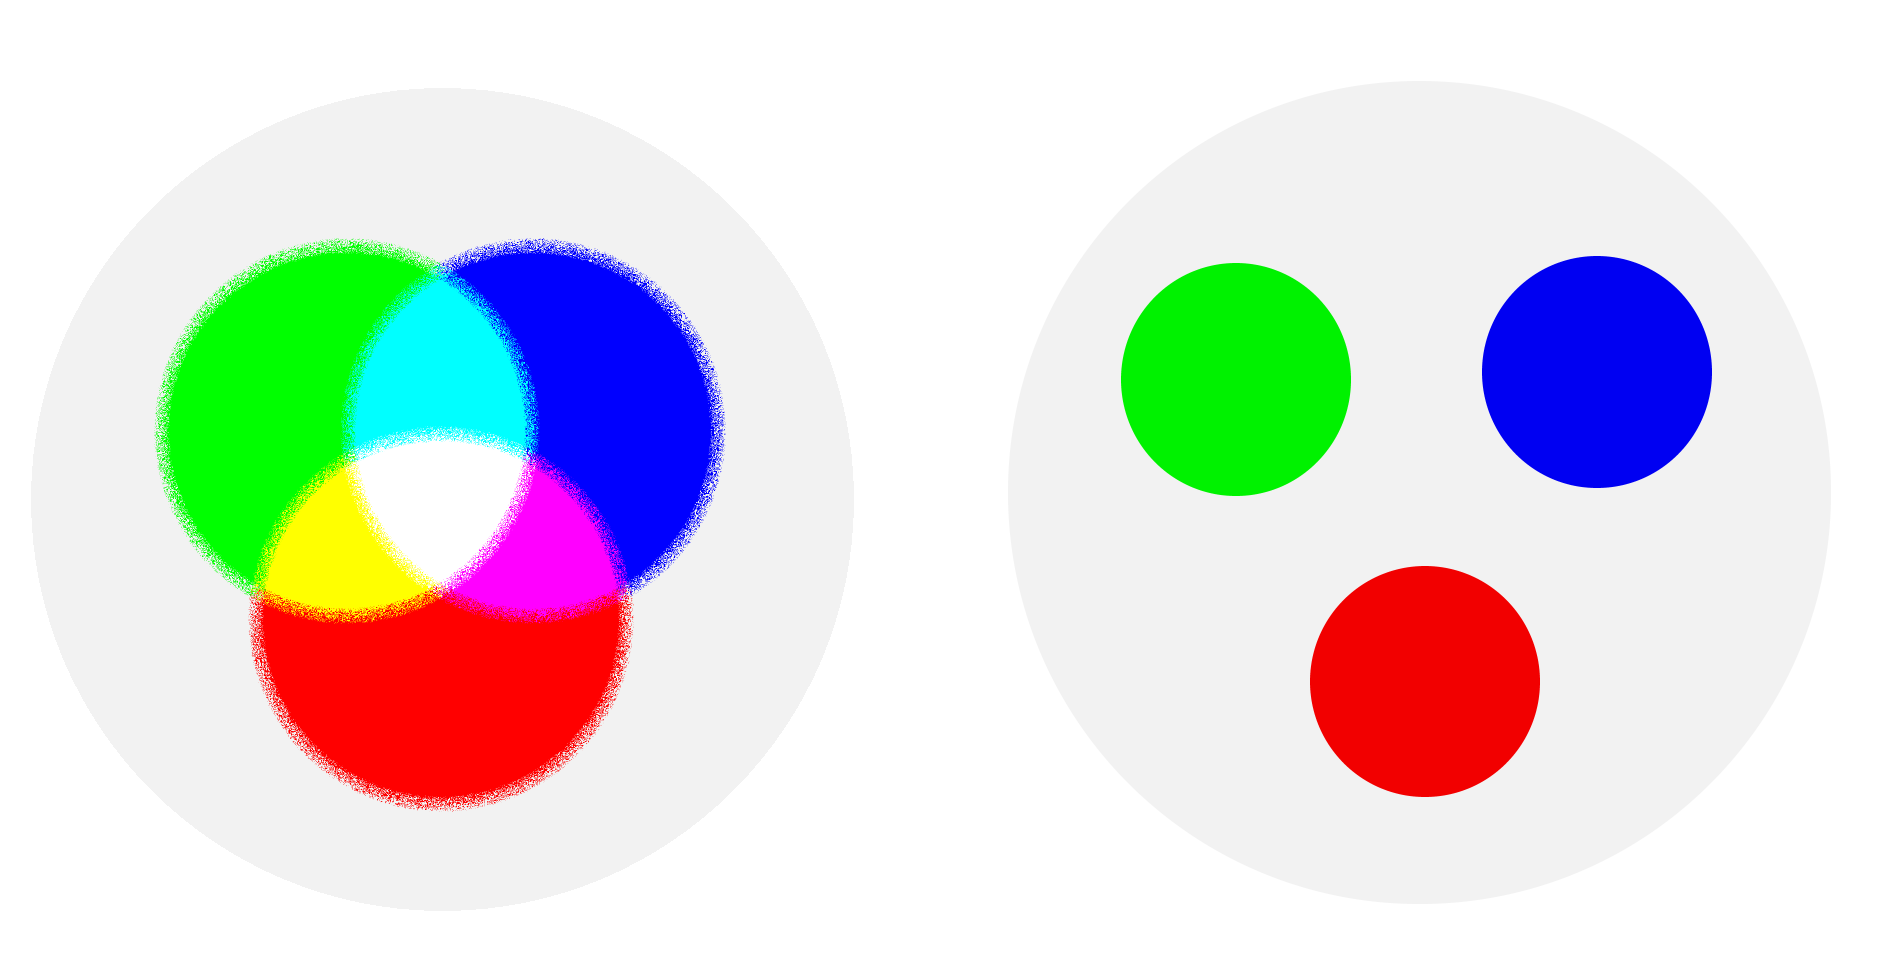
\includegraphics[width=0.8\textwidth]{Figures Introductory Lecture/Standard Model/GrayAdditiveColours.png}          
    %\caption{}                                                         
    \label{fig:strong_force_3}                                         
    \end{figure} \vspace{-0.5cm} \pause
    \ding{220} Insgesamt farbneutrale Teilchen!
\end{frame} 
%%%%%%%%%%%%%%%%%%%%%%%%%%%%%%%%%%%%%%%%%%%%%%%%%%%%%%%%%%%%%%%%%%%%%%%%%%%%%%%%%%%%%%%%%%%%%%
\begin{frame}{Das Standardmodell der Teilchenphysik}
% Idea is to show first only the particles student should know from the last slides, i.e. u and d quark. Then ask, what other elementary particles they might know of (expect electron and photon).
% From there talk about how physicists made the "strange" discovery of new particles that did not seem to be compsed out of ud only -> discovered more flavours over past decays, explain the three generations with increasing mass, same for leptons.
%In the end ask but how is it possible that the matter surrounding us is only made up of p,n ie ud quarks? -> Heavier flavoured particles must decay into first generation
\foreach \n in {1,...,4}{
    \includegraphics<\n>[width=0.9\textwidth]{Figures Introductory Lecture/Standard Model/SM_\n.png}%
}
%%%%%%%%%%%%%%%%%%%%%%%%%%%%%%%%%%%%%%%%%%%%%%%%%%%%%%%%%%%%%%%%%%%%%%%%%%%%%%%%%%%%%%%%%%%%%%
\end{frame}
\begin{frame}{Das Standardmodell der Teilchenphysik}
    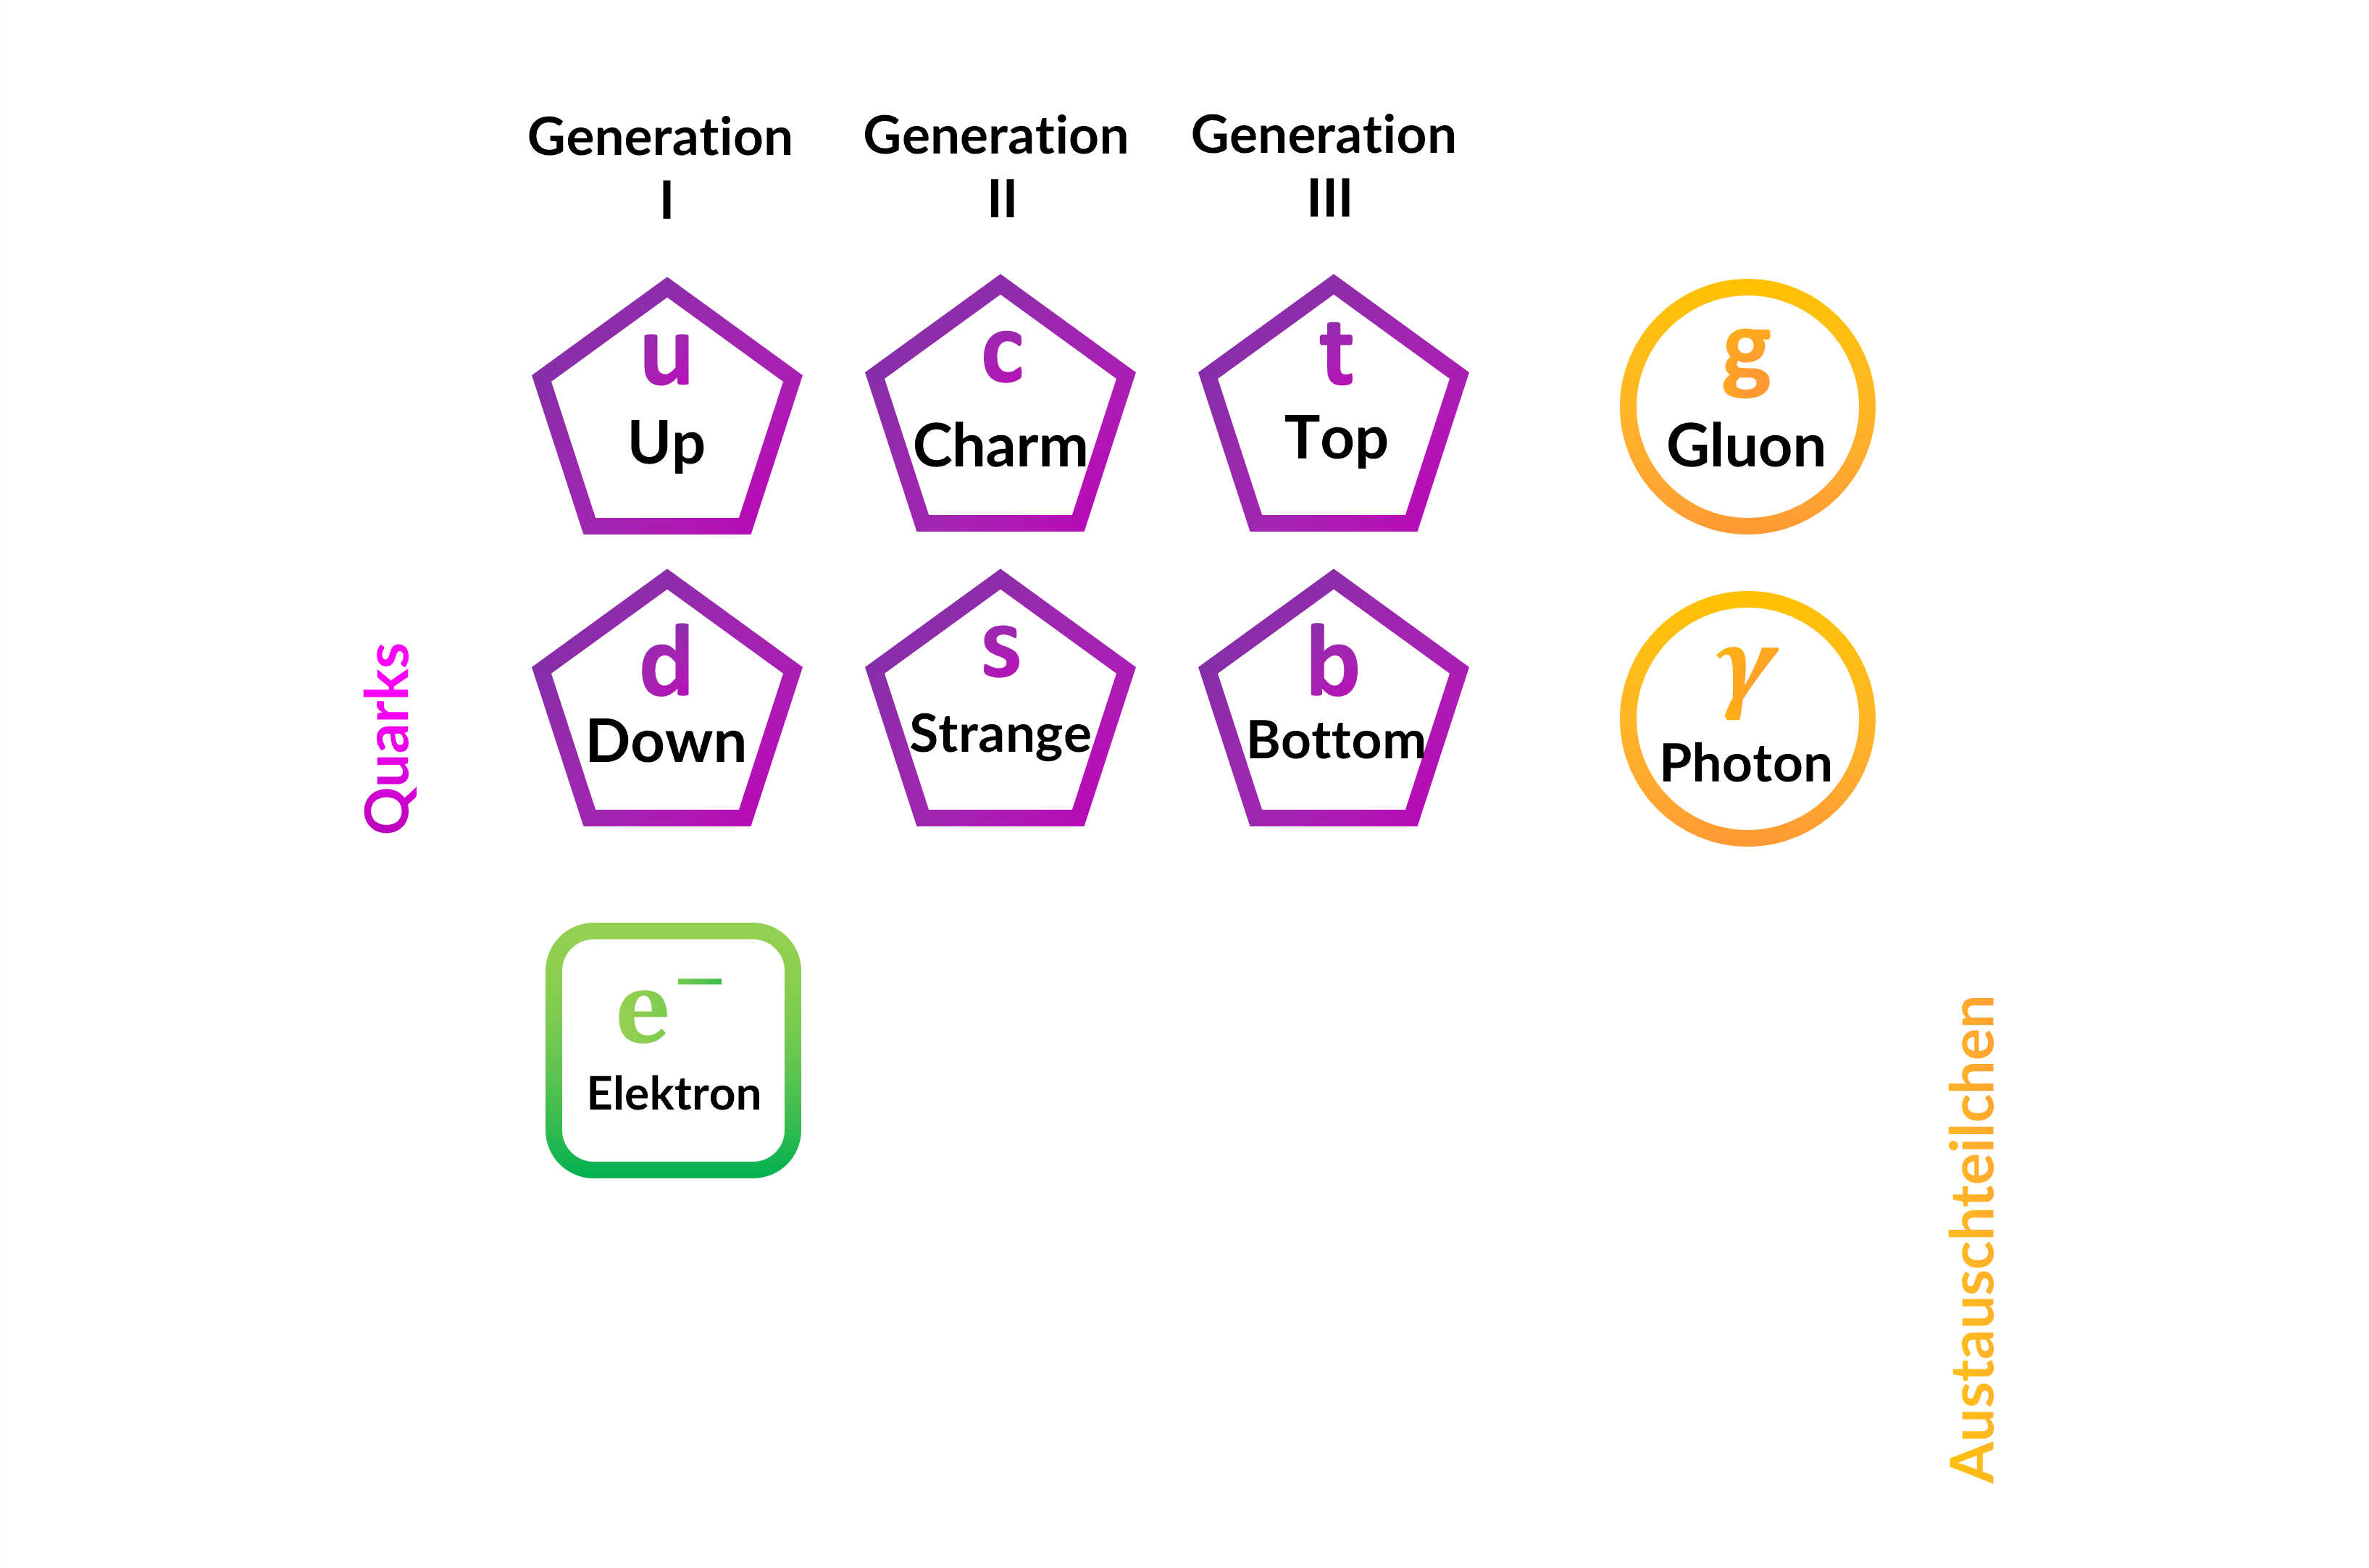
\includegraphics[width=0.9\textwidth]{Figures Introductory Lecture/Standard Model/SM2_1.png}
\end{frame}
%%%%%%%%%%%%%%%%%%%%%%%%%%%%%%%%%%%%%%%%%%%%%%%%%%%%%%%%%%%%%%%%%%%%%%%%%%%%%%%%%%%%%%%%%%%%%%

% \begin{frame}{Die schwache Wechselwirkung}
% % So how can we imagine such a decay? Lefthand side shows such a "strange" particle, what do we have to change to go a proton, is there something missing (charge) so need electrn for the decay.
% % More physical picture: show feynman diagram introduce bosons as mediators of interaction.
% \only<1>{
% \begin{figure}[htb]
%     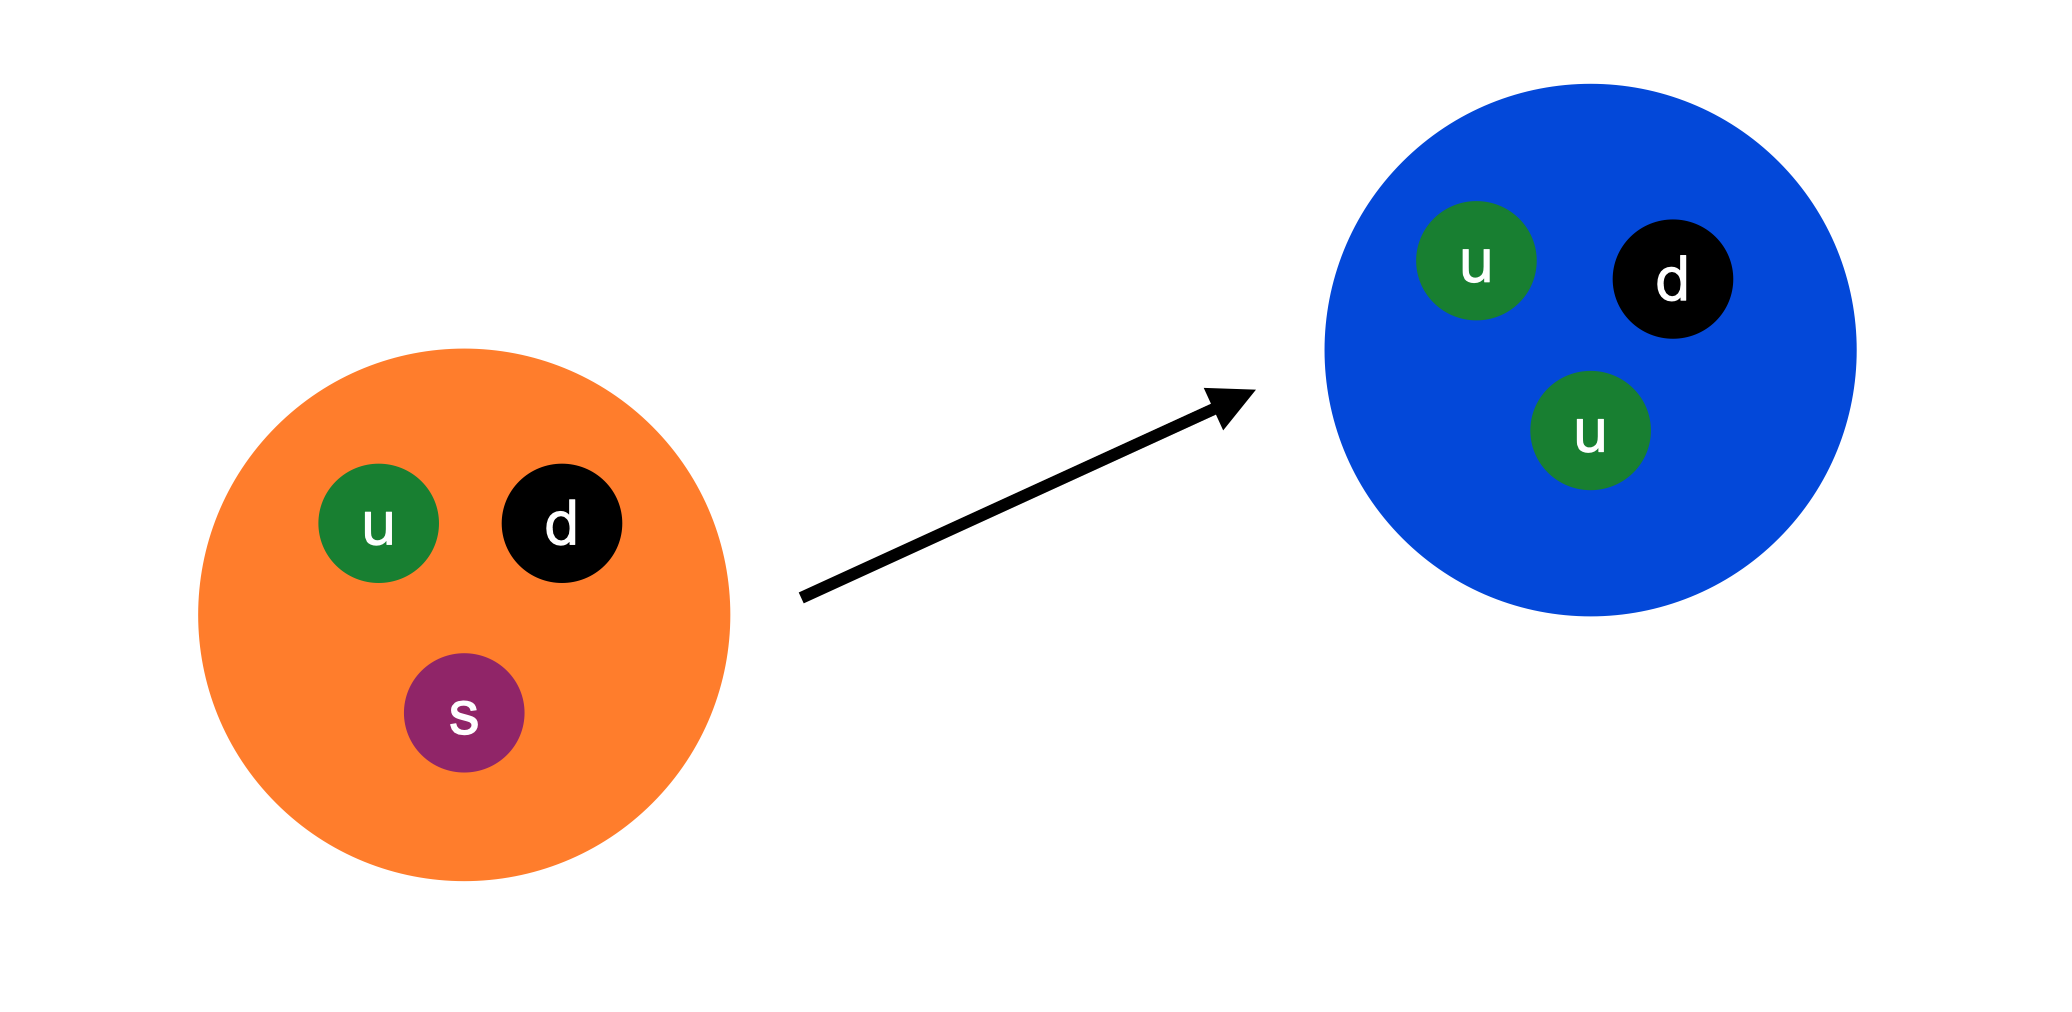
\includegraphics[width=0.9\textwidth]{Figures Introductory Lecture/Standard Model/LambdaDecay.png}%
%     %\caption{}
%     \label{fig:LambdaToProton}
% \end{figure}
% }
% \only<2>{
% \begin{figure}[htb]
%     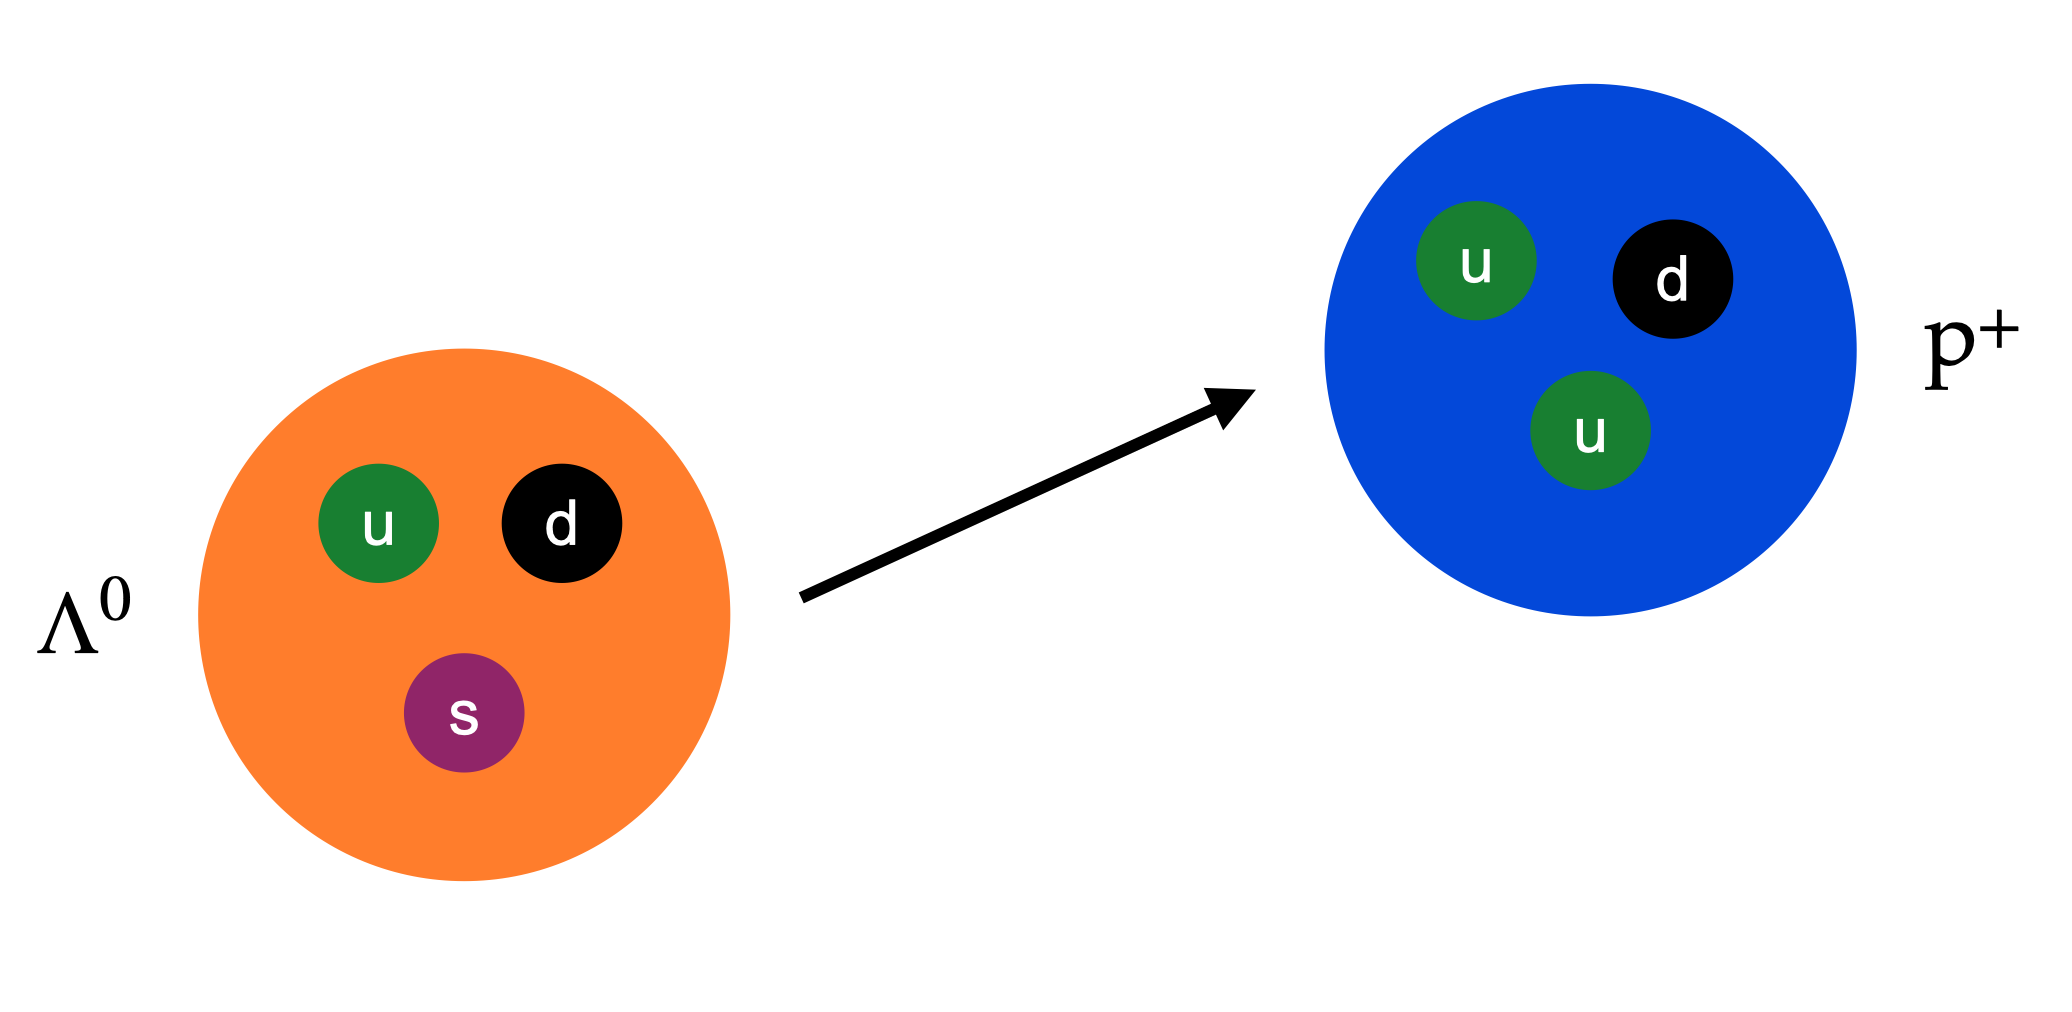
\includegraphics[width=0.9\textwidth]{Figures Introductory Lecture/Standard Model/LambdaDecayCharge.png}%
%     %\caption{}
%     \label{fig:Lambda_Decay}
% \end{figure}
% }
% \only<3>{
% \begin{figure}[htb]
%     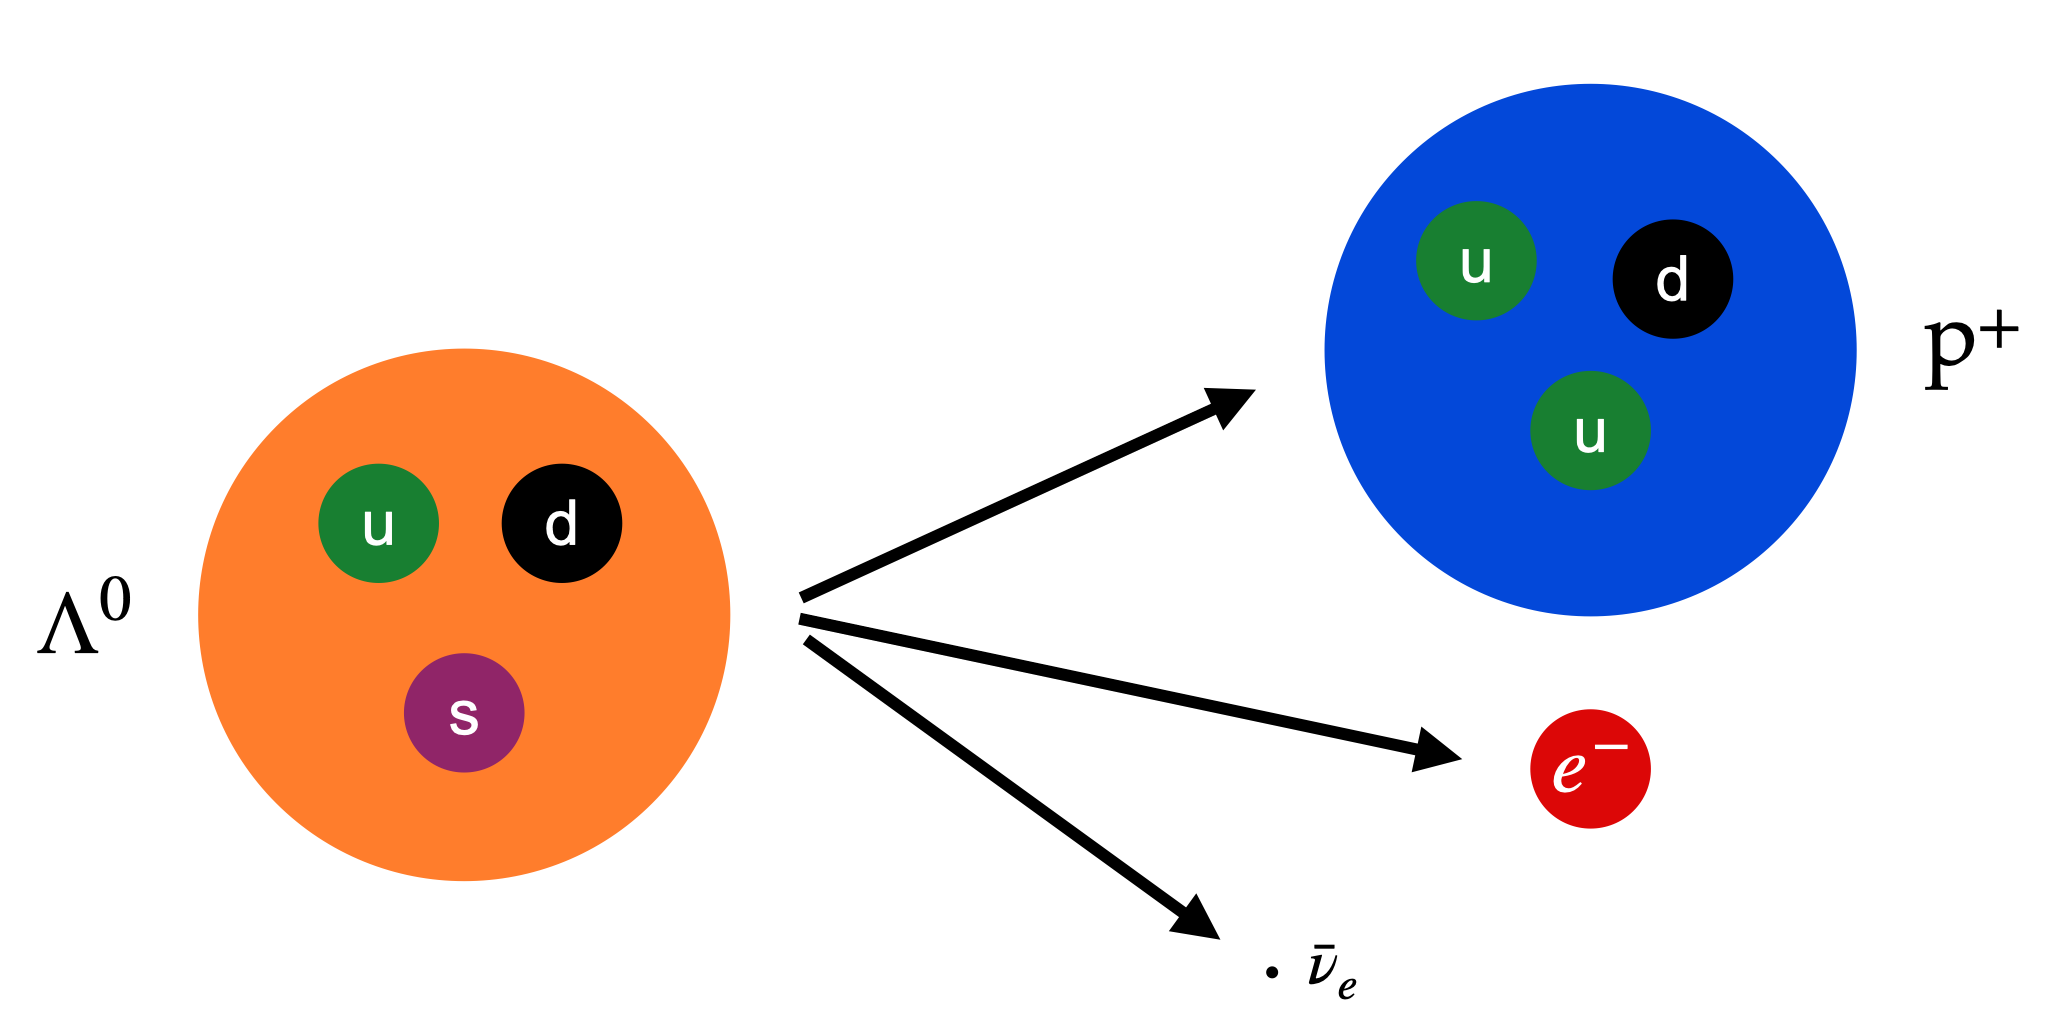
\includegraphics[width=0.9\textwidth]{Figures Introductory Lecture/Standard Model/LambdaDecayFull.png}%
%     %\caption{}
%     \label{fig:Lambda_DecayFull}
% \end{figure}
% }
% \end{frame}




\begin{frame}{Die schwache Wechelwirkung}
\begin{center}
    

    \begin{tikzpicture}[scale=0.9]
 
          \fill[orange] (0,0) circle (2) node [left=60pt,white] {\LARGE $\Lambda^0$};
          \fill[upQuark] (-0.75,-0.75) circle (0.5)  node[black] {\Large $u$};
            \fill[downQuark] (0.75,-0.75) circle (0.5)  node[white] {\Large$d$};
            \fill[strangeQuark] (0,0.75) circle (0.5)  node[black] {\Large$s$};

             \fill[Proton] (7,1) circle (2) node [right=60pt, white] {\LARGE $p$} ;
        \fill[upQuark] (6.25,0.25)circle (0.5)  node[black] {\Large$u$};
             \fill[upQuark] (7,1.75)circle (0.5)  node[black] {\Large$u$};
              \fill[downQuark] (7.75,0.25)circle (0.5)  node[white] {\Large$d$} ;


       % \fill[Elektron] (7.1,-2) circle (0.3) node[black] {$e^-$};


       % \fill[black] (6,-3) circle (0.05) node[right] {$\Bar{\nu}_e$};

        \draw[-{Latex[length=5mm]}, line width=1mm] (2.1,0.1) to (4.9,0.9){};
        %\draw[-{Latex[length=5mm]}, line width=1mm] (2.1,0) to (6.5,-1.8){};
      %  \draw[-{Latex[length=5mm]}, line width=1mm] (2.1,-0.1) to (5.9,-2.9){};
              
            
%Controling Points
\fill[white] (-3,-4) circle (0.1);
\fill[white] (10,3) circle (0.1);
    \end{tikzpicture}
    \end{center}
\end{frame}




\begin{frame}{Die schwache Wechelwirkung}\addtocounter{framenumber}{-1}
\begin{center}
    

    \begin{tikzpicture}[scale=0.9]
 
        \fill[orange] (0,0) circle (2) node [left=60pt,black] {\LARGE $\Lambda^0$};
            \fill[upQuark] (-0.75,-0.75) circle (0.5)  node[black] {\Large $u$};
            \fill[downQuark] (0.75,-0.75) circle (0.5)  node[white] {\Large$d$};
            \fill[strangeQuark] (0,0.75) circle (0.5)  node[black] {\Large$s$};

        \fill[Proton] (7,1) circle (2) node [right=60pt, black] {\LARGE $p$} ;
            \fill[upQuark] (6.25,0.25)circle (0.5)  node[black] {\Large$u$};
             \fill[upQuark] (7,1.75)circle (0.5)  node[black] {\Large$u$};
              \fill[downQuark] (7.75,0.25)circle (0.5)  node[white] {\Large$d$} ;


        %\fill[Elektron] (7.1,-2) circle (0.3) node[black] {$e^-$};


        %\fill[black] (6,-3) circle (0.05) node[right] {$\Bar{\nu}_e$};

        \draw[-{Latex[length=5mm]}, line width=1mm] (2.1,0.1) to (4.9,0.9){};
      %  \draw[-{Latex[length=5mm]}, line width=1mm] (2.1,0) to (6.5,-1.8){};
        %\draw[-{Latex[length=5mm]}, line width=1mm] (2.1,-0.1) to (5.9,-2.9){};
              
            
%Controling Points
\fill[white] (-3,-4) circle (0.1);
\fill[white] (10,3) circle (0.1);
    \end{tikzpicture}
    \end{center}
\end{frame}

\begin{frame}{Die schwache Wechelwirkung}\addtocounter{framenumber}{-1}
\begin{center}
    

    \begin{tikzpicture}[scale=0.9]
 
        \fill[orange] (0,0) circle (2) node [left=60pt,black] {\LARGE $\Lambda^0$};
            \fill[upQuark] (-0.75,-0.75) circle (0.5)  node[black] {\Large $u$};
            \fill[downQuark] (0.75,-0.75) circle (0.5)  node[white] {\Large$d$};
            \fill[strangeQuark] (0,0.75) circle (0.5)  node[black] {\Large$s$};

        \fill[Proton] (7,1) circle (2) node [right=60pt, black] {\LARGE $p$} ;
            \fill[upQuark] (6.25,0.25)circle (0.5)  node[black] {\Large$u$};
             \fill[upQuark] (7,1.75)circle (0.5)  node[black] {\Large$u$};
              \fill[downQuark] (7.75,0.25)circle (0.5)  node[white] {\Large$d$} ;


        \fill[Elektron] (7.1,-2) circle (0.3) node[black] {$e^-$};


        \fill[black] (6,-3) circle (0.05) node[right] {$\Bar{\nu}_e$};

        \draw[-{Latex[length=5mm]}, line width=1mm] (2.1,0.1) to (4.9,0.9){};
        \draw[-{Latex[length=5mm]}, line width=1mm] (2.1,0) to (6.5,-1.8){};
        \draw[-{Latex[length=5mm]}, line width=1mm] (2.1,-0.1) to (5.9,-2.9){};
              
            
%Controling Points
\fill[white] (-3,-4) circle (0.1);
\fill[white] (10,3) circle (0.1);
    \end{tikzpicture}
    \end{center}
\end{frame}

%%%%%%%%%%%%%%%%%%%%%%%%%%%%%%%%%%%%%%%%%%%%%%%%%%%%%%%%%%%%%%%%%%%%%%%%%%%%%%%%%%%%%%%%%%%%%%
\begin{frame}{Feynman Diagramme}
% Anstelle solcher Kugel bilder verwenden Physiker:innen Feynman diagramme
\begin{center}
\begin{tikzpicture}
\begin{feynman}
    \vertex(ul) {\(u\)};
    \vertex[right=5cm of ul] (ur) {\(u\)};
    \vertex[below=0.75cm of ul] (dl) {\(d\)};
    \vertex[right=5cm of dl] (dr) {\(d\)};
    \vertex[below=0.75cm of dl] (sl) {\(s\)};
    \vertex[right=5cm of sl] (ur2) {\(u\)};
    \vertex[right=2cm of sl] (W1);
    \vertex[below right = 1cm and 1.5cm of W1] (W2);
    \vertex[below = 0.5cm of ur2] (e) {\(e^-\)};
    \vertex[below = 1cm of e] (nue) {\(\bar \nu_e\)};
    \diagram* { {[edges=fermion]
    (ul) -- (ur), (dl) -- (dr), (sl) -- (ur2),
    (W2) -- (e), (nue) -- (W2)};
    (W1) -- [boson, edge label' = \(W^-\)] (W2)
    };
\draw [decoration={brace}, decorate]  (sl.south west) -- (ul.north west) node [pos=0.5, left] {\(\Lambda^0\)};
\draw [decoration={brace}, decorate] (ur.north east) --  (ur2.south east) node [pos=0.5, right] {\(p^+\)};
\end{feynman}
\end{tikzpicture}   
\end{center}
\ding{43} Nur die schwache Wechselwirkung ist in der Lage den \textbf{Flavour} eines Teilchens zu verändern! 
\end{frame}
%%%%%%%%%%%%%%%%%%%%%%%%%%%%%%%%%%%%%%%%%%%%%%%%%%%%%%%%%%%%%%%%%%%%%%%%%%%%%%%%%%%%%%%%%%%%%%%


\begin{frame}[fragile]{Das Standardmodell der Teilchenphysik II}
% Show the full SM, talk about bosons as mediators, maybe the example of two people on skateboards throwing a ball, as example for repulsive force via mediating particle?

    % - Higgs und Fragen zur Gravitation vorbereiten? -> würde ich weglassen, nicht wirklich relevant, eher das Higgs kurz erwähnen als das elementarteilchen das als letztes gefunden wurde und den Punkt machen, dass Teilchenphysik aktuell ist und nicht nur experimente von vor 100 Jahren

\foreach \n in {1,...,9}{
        \includegraphics<\n>[width=0.9\textwidth]{Figures Introductory Lecture/Standard Model/SM2_\n.png}%
} 
%%%%%%%%%%%%%%%%%%%%%%%%%%%%%%%%%%%%%%%%%%%%%%%%%%%%%%%%%%%%%%%%%%%%%%%%%%%%%%%%%%%%%%%%%%%%%%
\end{frame}
\begin{frame}{Standardmodell: Das wichtigste für heute}
\begin{itemize}
    \item 6 Quark-Flavours  $u$, $d$,$s$, $c$, $b$, $t$
    \item starke-, schwache- und elektromagnetische Kraft
    \item Flavour-Änderung nur über Schwachen Zerfall
    \item Austauschteilchen $\gamma$, $Z^0$ \& $W^{\pm}$, $g$
    \item Farbladung als Ladung der starken Kraft
    \item Quarks farbgeladen, Teilchen farbneutral
    \item []
    \item[\ding{43}] Starke Kraft recht unverstanden und Objekt aktueller Forschung!
\end{itemize}
    
\end{frame}
%%%%%%%%%%%%%%%%%%%%%%%%%%%%%%%%%%%%%%%%%%%%%%%%%%%%%%%%%%%%%%%%%%%%%%%%%%%%%%%%%%%%%%%%%%%%%%
  \begin{frame}{Was ist Materie, wie kann man sie "messen"?}\Large
 Und jetzt?
 \begin{itemize}
     \item Wie kann man Teilchen erzeugen?
     \item Wie können wir das alles nachweisen?!
 \end{itemize}
\begin{center} \pause
 
Aber erstmal \\   \textbf{\textcolor{red}{5\,min Pause :)}
}
\end{center}  
\end{frame}
%%%%%%%%%%%%%%%%%%%%%%%%%%%%%%%%%%%%%%%%%%%%%%%%%%%%%%%%%%%%%%%%%%%%%%%%%%%%%%%%%%%%%%%%%%%%%% 
   \section{LHCb-Detektor am CERN}
\begin{frame}[plain]

\begin{center} 
  \huge{  \ding{183} }\\
   \Large{ Einführung in den LHCb-Detektor am CERN}

\end{center}
\end{frame}
%%%%%%%%%%%%%%%%%%%%%%%%%%%%%%%%%%%%%%%%%%%%%%%%%%%%%%%%%%%%%%%%%%%%%%%%%%%%%%%%%%%%%%%%%%%%%%


\begin{frame}{Ein Teilchen bitte!}

    \begin{center}
   \Large Wir wollen Teilchen produzieren!\\
    
    \Large Dazu brauchen wir viel \textbf{\textcolor{red}{Energie}}!
   \mathrm{ \begin{align*}
        \textcolor{red}{E} = m\cdot c^\textsf{2} 
    \end{align*}
    }
        
    \end{center}
    
\end{frame}
%%%%%%%%%%%%%%%%%%%%%%%%%%%%%%%%%%%%%%%%%%%%%%%%%%%%%%%%%%%%%%%%%%%%%%%%%%%%%%%%%%%%%%%%%%%%%%
\subsection{Bild: CERN, verändert}
\begin{frame}{Willkommen am CERN \& LHC}

  \begin{center}
   \Large Wie kann man die benötigte Energie bereitstellen?
    \end{center}
    
    \begin{figure}[h]
        \centering
        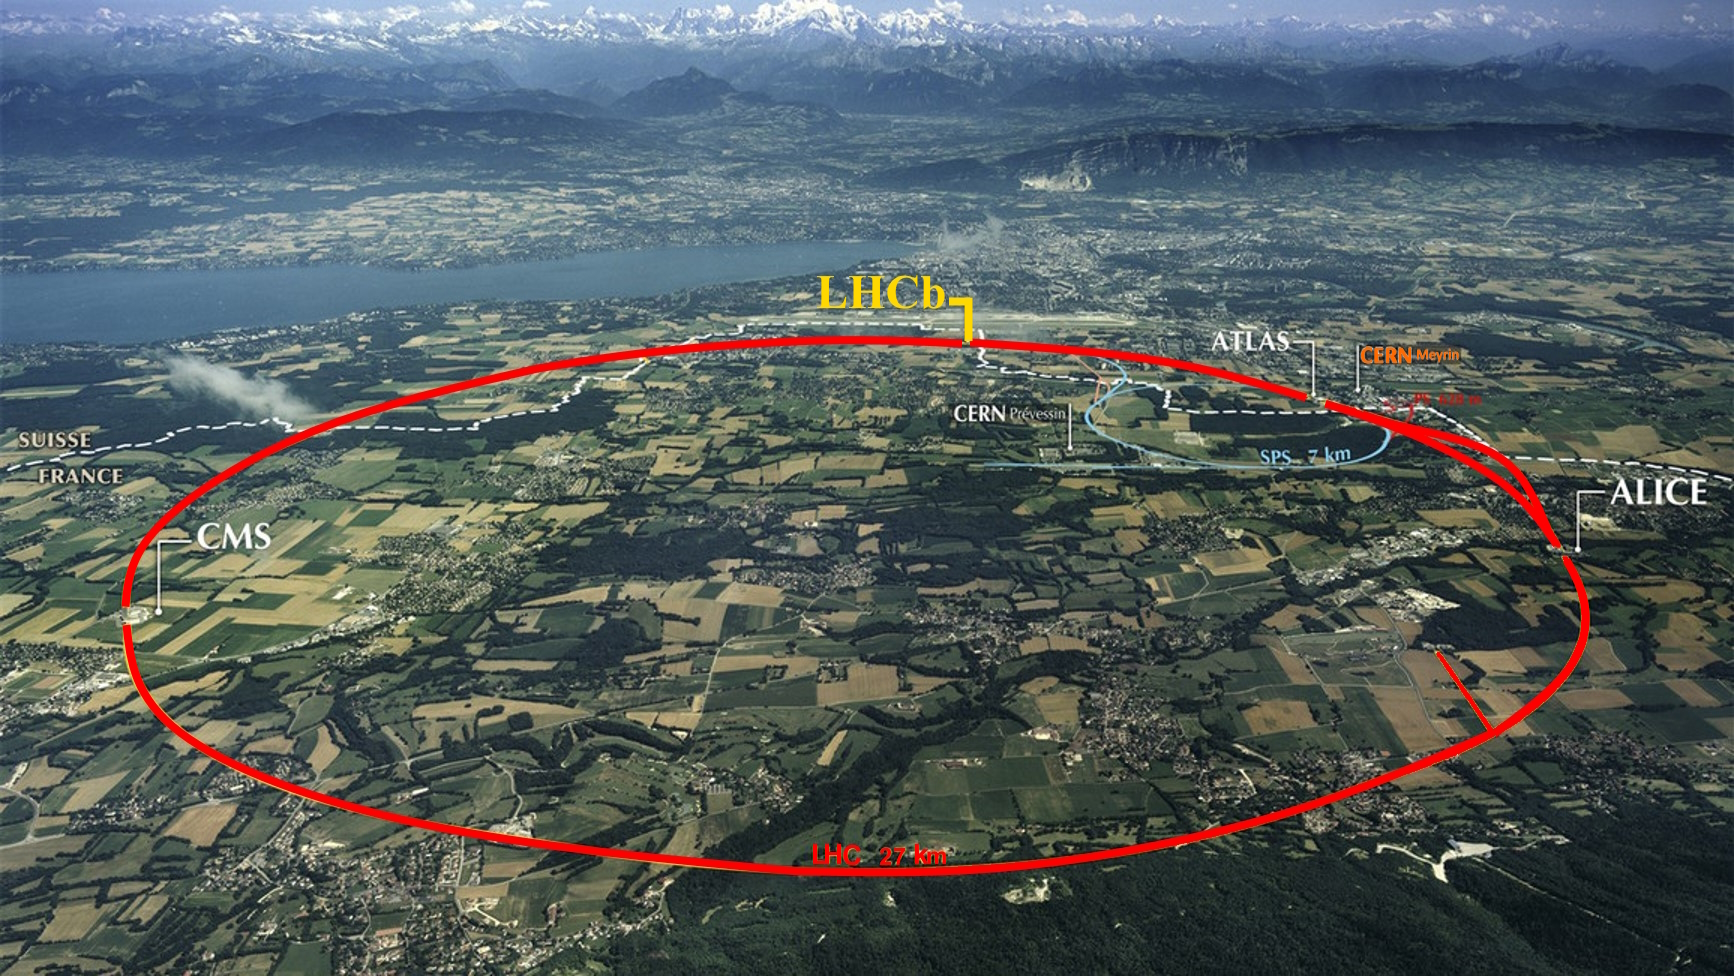
\includegraphics[width=0.7\textwidth]{Figures Introductory Lecture/LHCb Detector/LHC.jpg}
        %\c%aption{https://visit.cern/node/616}
        \label{fig:CERN_LHC}
    \end{figure}
\end{frame}

%%%%%%%%%%%%%%%%%%%%%%%%%%%%%%%%%%%%%%%%%%%%%%%%%%%%%%%%%%%%%%%%%%%%%%%%%%%%%%%%%%%%%%%%%%%%%%
\begin{frame}
\begin{figure}
\begin{overpic}[width=\textwidth]{Figures Introductory Lecture/LHCb Detector/LHC.jpg}
     \put (55,43.5) {\tiny \textcolor{white}{\centering \rotatebox[]{270}{$\rightarrow$}  Genf}}
     \put (10,39) {\tiny \textcolor{white}{Genfer See}}
     \put (0,50)  {\tiny \textcolor{white}{$\leftarrow$ Lausanne}}
        \put (92,5)  {\tiny \textcolor{white}{ Lyon \rotatebox[]{340}{$\rightarrow$}}}
        \put (47,54) {\tiny \textcolor{ black}{\rotatebox[]{135}{\ding{43}} Mont Blanc}}
\end{overpic}
\end{figure}
\end{frame}
%%%%%%%%%%%%%%%%%%%%%%%%%%%%%%%%%%%%%%%%%%%%%%%%%%%%%%%%%%%%%%%%%%%%%%%%%%%%%%%%%%%%%%%%%%%%%%
\begin{frame}\addtocounter{framenumber}{-1}
\begin{figure}
\begin{overpic}[width=\textwidth]{Figures Introductory Lecture/LHCb Detector/LHC+GVA.jpg}
        \put (44,43.5) {\tiny \parbox{2.5cm}{\textcolor{white}{\centering \rotatebox[]{45}{\ding{40}} Flughafen Genf\\ Landebahnlänge: 4\,km}}}
        %\put (90,36)  {\tiny \textcolor{green}{TGV}}
        \put (0,50)  {\tiny \textcolor{white}{$\leftarrow$ Lausanne}}
        \put (92,5)  {\tiny \textcolor{white}{ Lyon \rotatebox[]{340}{$\rightarrow$}}}
        \put (10,39) {\tiny \textcolor{white}{Genfer See}}
        \put (47,54) {\tiny \textcolor{ black}{\rotatebox[]{135}{\ding{43}} Mont Blanc}}
\end{overpic}
\end{figure}
\end{frame}
%%%%%%%%%%%%%%%%%%%%%%%%%%%%%%%%%%%%%%%%%%%%%%%%%%%%%%%%%%%%%%%%%%%%%%%%%%%%%%%%%%%%%%%%%%%%%%
\begin{frame}\addtocounter{framenumber}{-1}
\begin{figure}
\begin{overpic}[width=\textwidth]{Figures Introductory Lecture/LHCb Detector/LHC+GVA+TGV.jpg}
        \put (44,43.5) {\tiny \parbox{2.5cm}{\textcolor{white}{\centering \rotatebox[]{45}{\ding{40}} Flughafen Genf\\ Landebahnlänge: 4\,km}}}
        \put (90,36)  {\tiny \textcolor{green}{TGV}}
        \put (0,50)  {\tiny \textcolor{white}{$\leftarrow$ Lausanne}}
        \put (92,5)  {\tiny \textcolor{white}{ Lyon \rotatebox[]{340}{$\rightarrow$}}}
        \put (10,39) {\tiny \textcolor{white}{Genfer See}}
        \put (47,54) {\tiny \textcolor{ black}{\rotatebox[]{135}{\ding{43}} Mont Blanc}}
\end{overpic}
\end{figure}
\end{frame}

\begin{frame}{LHC vs. ICE}
\begin{spacing}{2}
       \textbf{ Energie pro Strahl: 350\,MJ } \\
   \begin{itemize}
       \item[\ding{43}] ICE ($m=400\,t$) bei 150\,$\nicefrac{\text{km}}{\text{h}}$ \\ 
       \item[\ding{43}] Nährwert 153 Tafeln Schokolade\\ 
   \end{itemize}

     \textbf{Energie pro Proton: 1\,\text{µJ} } \\
   \begin{itemize}
       \item[\ding{43}] Biene ($m=0.1\,g$) bei 1\,$\nicefrac{\text{km}}{\text{h}}$ 
   \end{itemize}
   
\end{spacing}

   
    
\end{frame}
%%%%%%%%%%%%%%%%%%%%%%%%%%%%%%%%%%%%%%%%%%%%%%%%%%%%%%%%%%%%%%%%%%%%%%%%%%%%%%%%%%%%%%%%%%%%%%
%\begin{frame}{Motivation of Colider experiments (Production)}
%    E=m
    %    Wir benoetigen ein Experiment um schwere Teilchen (die nicht nur u und d enthalten) zu produzieren. Hierzu brauche wir viel Energie. % Eventuell Referenz zur kleinsten Wirkung (s.o.)?
%\end{frame}

%\begin{frame}{CERN, LHC, LHCb...}
%-> how can we produce the high amount of energy we need?
%    - From E=m. Huge Energy has to go somewhere when two particles (pp) are colliding.
%    - start with linear collider than round. Synchrotron Principe
%    - charged particles in a magn. field got accelerated
%    - Proton has more energy than a.i. Electrons. (ref to Bonn: e+ e-)
    % Das intuitive Verständnis, dass bei anihilation von Elektron und Positron "Energie frei wird", kann eventuell aufRückfragen stoßen, wenn wir pp Kollision haben, insbesondere wenn wir keine See-Quarks einfürhen. Rückfragen müsste man mit einem neuen konzept entgegnen, das kann schnell in eine verwirrende richung fühen. Daher eventuell "falsche" Erklärung hier nutzen?
%\end{frame}
%%%%%%%%%%%%%%%%%%%%%%%%%%%%%%%%%%%%%%%%%%%%%%%%%%%%%%%%%%%%%%%%%%%%%%%%%%%%%%%%%%%%%%%%%%%%%%
\subsection{}
\begin{frame}{Die Kollision der Teilchen}%{Collision and Detection}
 %- Lot Energy has to go somewhere. (E=const.)
 %- Lot Energy, lot stuff, has to go somewhere. To what? Has to be figured out. -> 
Die hochenergetischen Teilchen kollidieren\\
\ding{43}  Was geschieht mit der Energie? % Energieerhaltung
 \\ 
%event display?
% Bild ist von hier: https://www.physicsmasterclasses.org/exercises/bonn1/de/teilchenkollision.htm
% koennte noch schoener gemacht werden. Aber die Idee ist vielleicht nicht schlecht.
\begin{figure}[h]
        %\centering
       
       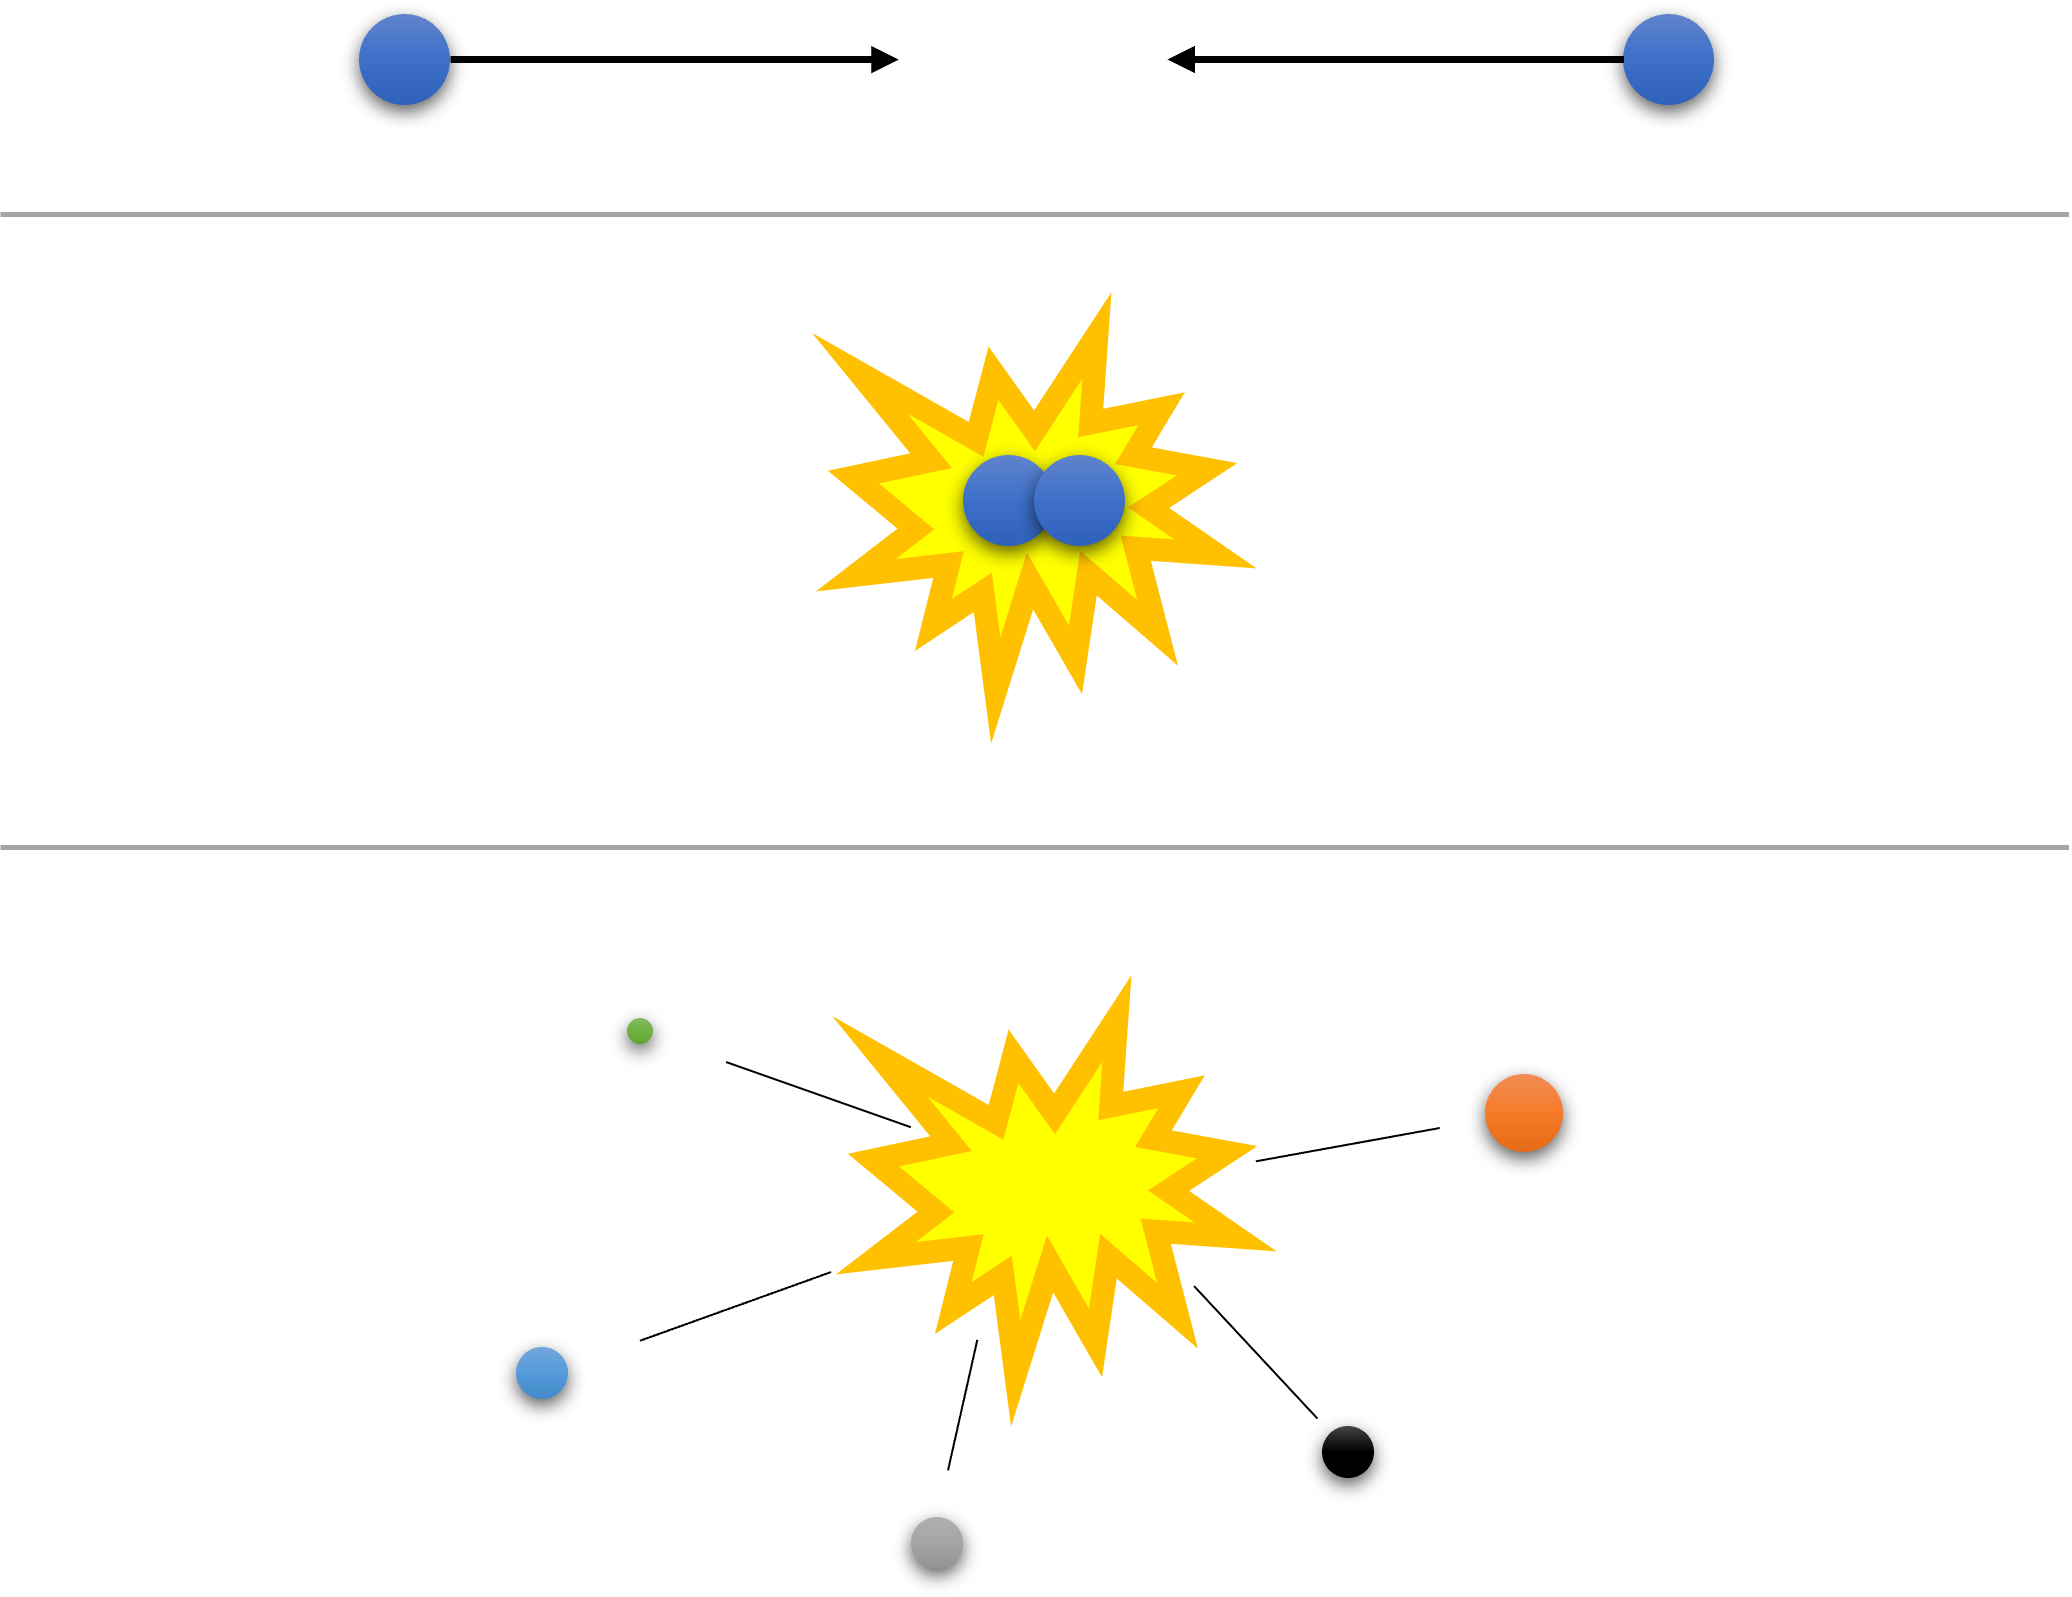
\includegraphics[width=0.43\textwidth]{Figures Introductory Lecture/LHCb Detector/Kollision.png}
        \label{fig:Kollision}
    \end{figure}
\end{frame}
%%%%%%%%%%%%%%%%%%%%%%%%%%%%%%%%%%%%%%%%%%%%%%%%%%%%%%%%%%%%%%%%%%%%%%%%%%%%%%%%%%%%%%%%%%%%%%%%
\begin{frame}{Detektive für Teilchen}\addtocounter{framenumber}{-1}
%- Da ist was Produziert wurden, wie kann man das Nachvollziehen. 
%    - Teilcehn treffen auf Material, diese Interaktion mit Material (-Schichten) kann man nachweisen und Spuren rekonstruieren
Wie können wir feststellen, was bei der Kollision passiert ist?\\
\ \\
    \begin{figure}[h]
        %\centering

        \begin{overpic}[width=0.8\textwidth]{Figures Introductory Lecture/LHCb Detector/Detectorsignal.png}
        \put(65,8){\tiny Auslesesystem}
        \put(45,50){\scriptsize Detektor}
        \put(44,0){\scriptsize \parbox{2cm}{Elektrisches Signal}}
        
        \end{overpic}
   
    \end{figure}
% Bild kann vermutlich auch noch in schoen erstellt werden :-D
% Ich finde das bild wunderschön

    \begin{itemize}
        \item<2-> Welches Signal gehört zu welchem Teilchen?
    \end{itemize}
    
\end{frame}
%%%%%%%%%%%%%%%%%%%%%%%%%%%%%%%%%%%%%%%%%%%%%%%%%%%%%%%%%%%%%%%%%%%%%%%%%%%%%%%%%%%%%%%%%%%%%%
%\begin{frame}{Welches Signal gehört zu welchem Teilchen?}
       %Wie kann man Teilchen anhand von Spuren unterscheiden? 
       %-> (Reminder) Ladung, Masse, Art der WW, Energie
       %-> Detektor hat verschiedene Teilce mit verschiedenen Aufgaben

%Fragende Enntwicklung: Wie kann man verschiedene Eigenschaften der Teichen herausfinden?
%\end{frame}
%%%%%%%%%%%%%%%%%%%%%%%%%%%%%%%%%%%%%%%%%%%%%%%%%%%%%%%%%%%%%%%%%%%%%%%%%%%%%%%%%%%%%%%%%%%%%%
\begin{frame}{Welches Signal gehört zu welchem Teilchen?}
    

\ \\
Erinnert euch an die Eigenschaften der Teilchen, die ihr kennt: \\
\begin{itemize}
    \item<2-> Masse \hfill $m$ \hspace{6cm}\,
    \item<2-> Elektrische Ladung  \hfill $q$ \hspace{6cm}\,
    \item<2-> Energie  \hfill $E$ \hspace{6cm}\,
    \item<2-> Impuls  \hfill $\vec{p} $ \hspace{6cm}\,
    \item<2-> Geschwindigkeit  \hfill $\vec{v}$ \hspace{6cm}\,
 
\ \\
    \item<3->[\ding{220}] Wie können wir mit dem LHCb-Detektor diese Eigenschaften messen?

    
\end{itemize}
\end{frame}
%%%%%%%%%%%%%%%%%%%%%%%%%%%%%%%%%%%%%%%%%%%%%%%%%%%%%%%%%%%%%%%%%%%%%%%%%%%%%%%%%%%%%%%%%%%%%%
% Im Folgenden ist die Überlegung: Der LHCb Detekor baut sich langsam auf. Auf den Slides sind immer die Geräte eingezeichnet und werden laufend ergänzt (Grafiken kann Lukas machen!), Außerdem hier Bilder von den jeweligen Geräten, s. Slides von Sebastian/Klaas. Ziel ist die Abbildung auf der Rechenaufgabe 

%idee hierfür: beispiel teilchen durch detektor folgen (z.B. b meson wegen namensgebung):
%- zerfall im velo: gute ortsauflösung
%- rich 1: impulsmessung
%- tt: verbindung zu velo spur
%- magnet: ablenken geladener teilchen
%- tracking stations: ort nach ablenkung im magnet 
%- rich2: impuls messung von höherem impuls mit anderem gas
%- ecal/ hcal: teilchen stoppen und energie messen
%- muonkammern: misst spuren von teilchen die nicht im calo gestoppt werden (kann man auch weglassen)

%idee der folgenden slides: lhcb detektor baut sich stück für stück vom kollisionspunkt an auf, jede slide hat unten die schematik vom bisherigen detektor und oben ein foto vom subdetektor, den die slide erklärt. zusätzlich hat jede slide ein paar stichpunkte zur funktionsweise des detektors. für einige slides bieten sich fragen an die schüler an (als kommentare an den stichpunkten hinterlegt) 
%%%%%%%%%%%%%%%%%%%%%%%%%%%%%%%%%%%%%%%%%%%%%%%%%%%%%%%%%%%%%%%%%%%%%%%%%%%%%%%%%%%%%%%%%%%%%%
\subsection{Bild: CERN}
\begin{frame}{Vertex Locator (VELO)}
    \begin{minipage}{0.58\textwidth}
        \begin{itemize}
        \item Um den Kollisionspunkt positioniert
        \item Wichtig für Spurrekonstruktion
    \end{itemize}
    \end{minipage}\hfill
    \begin{minipage}{0.38\textwidth}
        \begin{figure}[h]
        \centering
        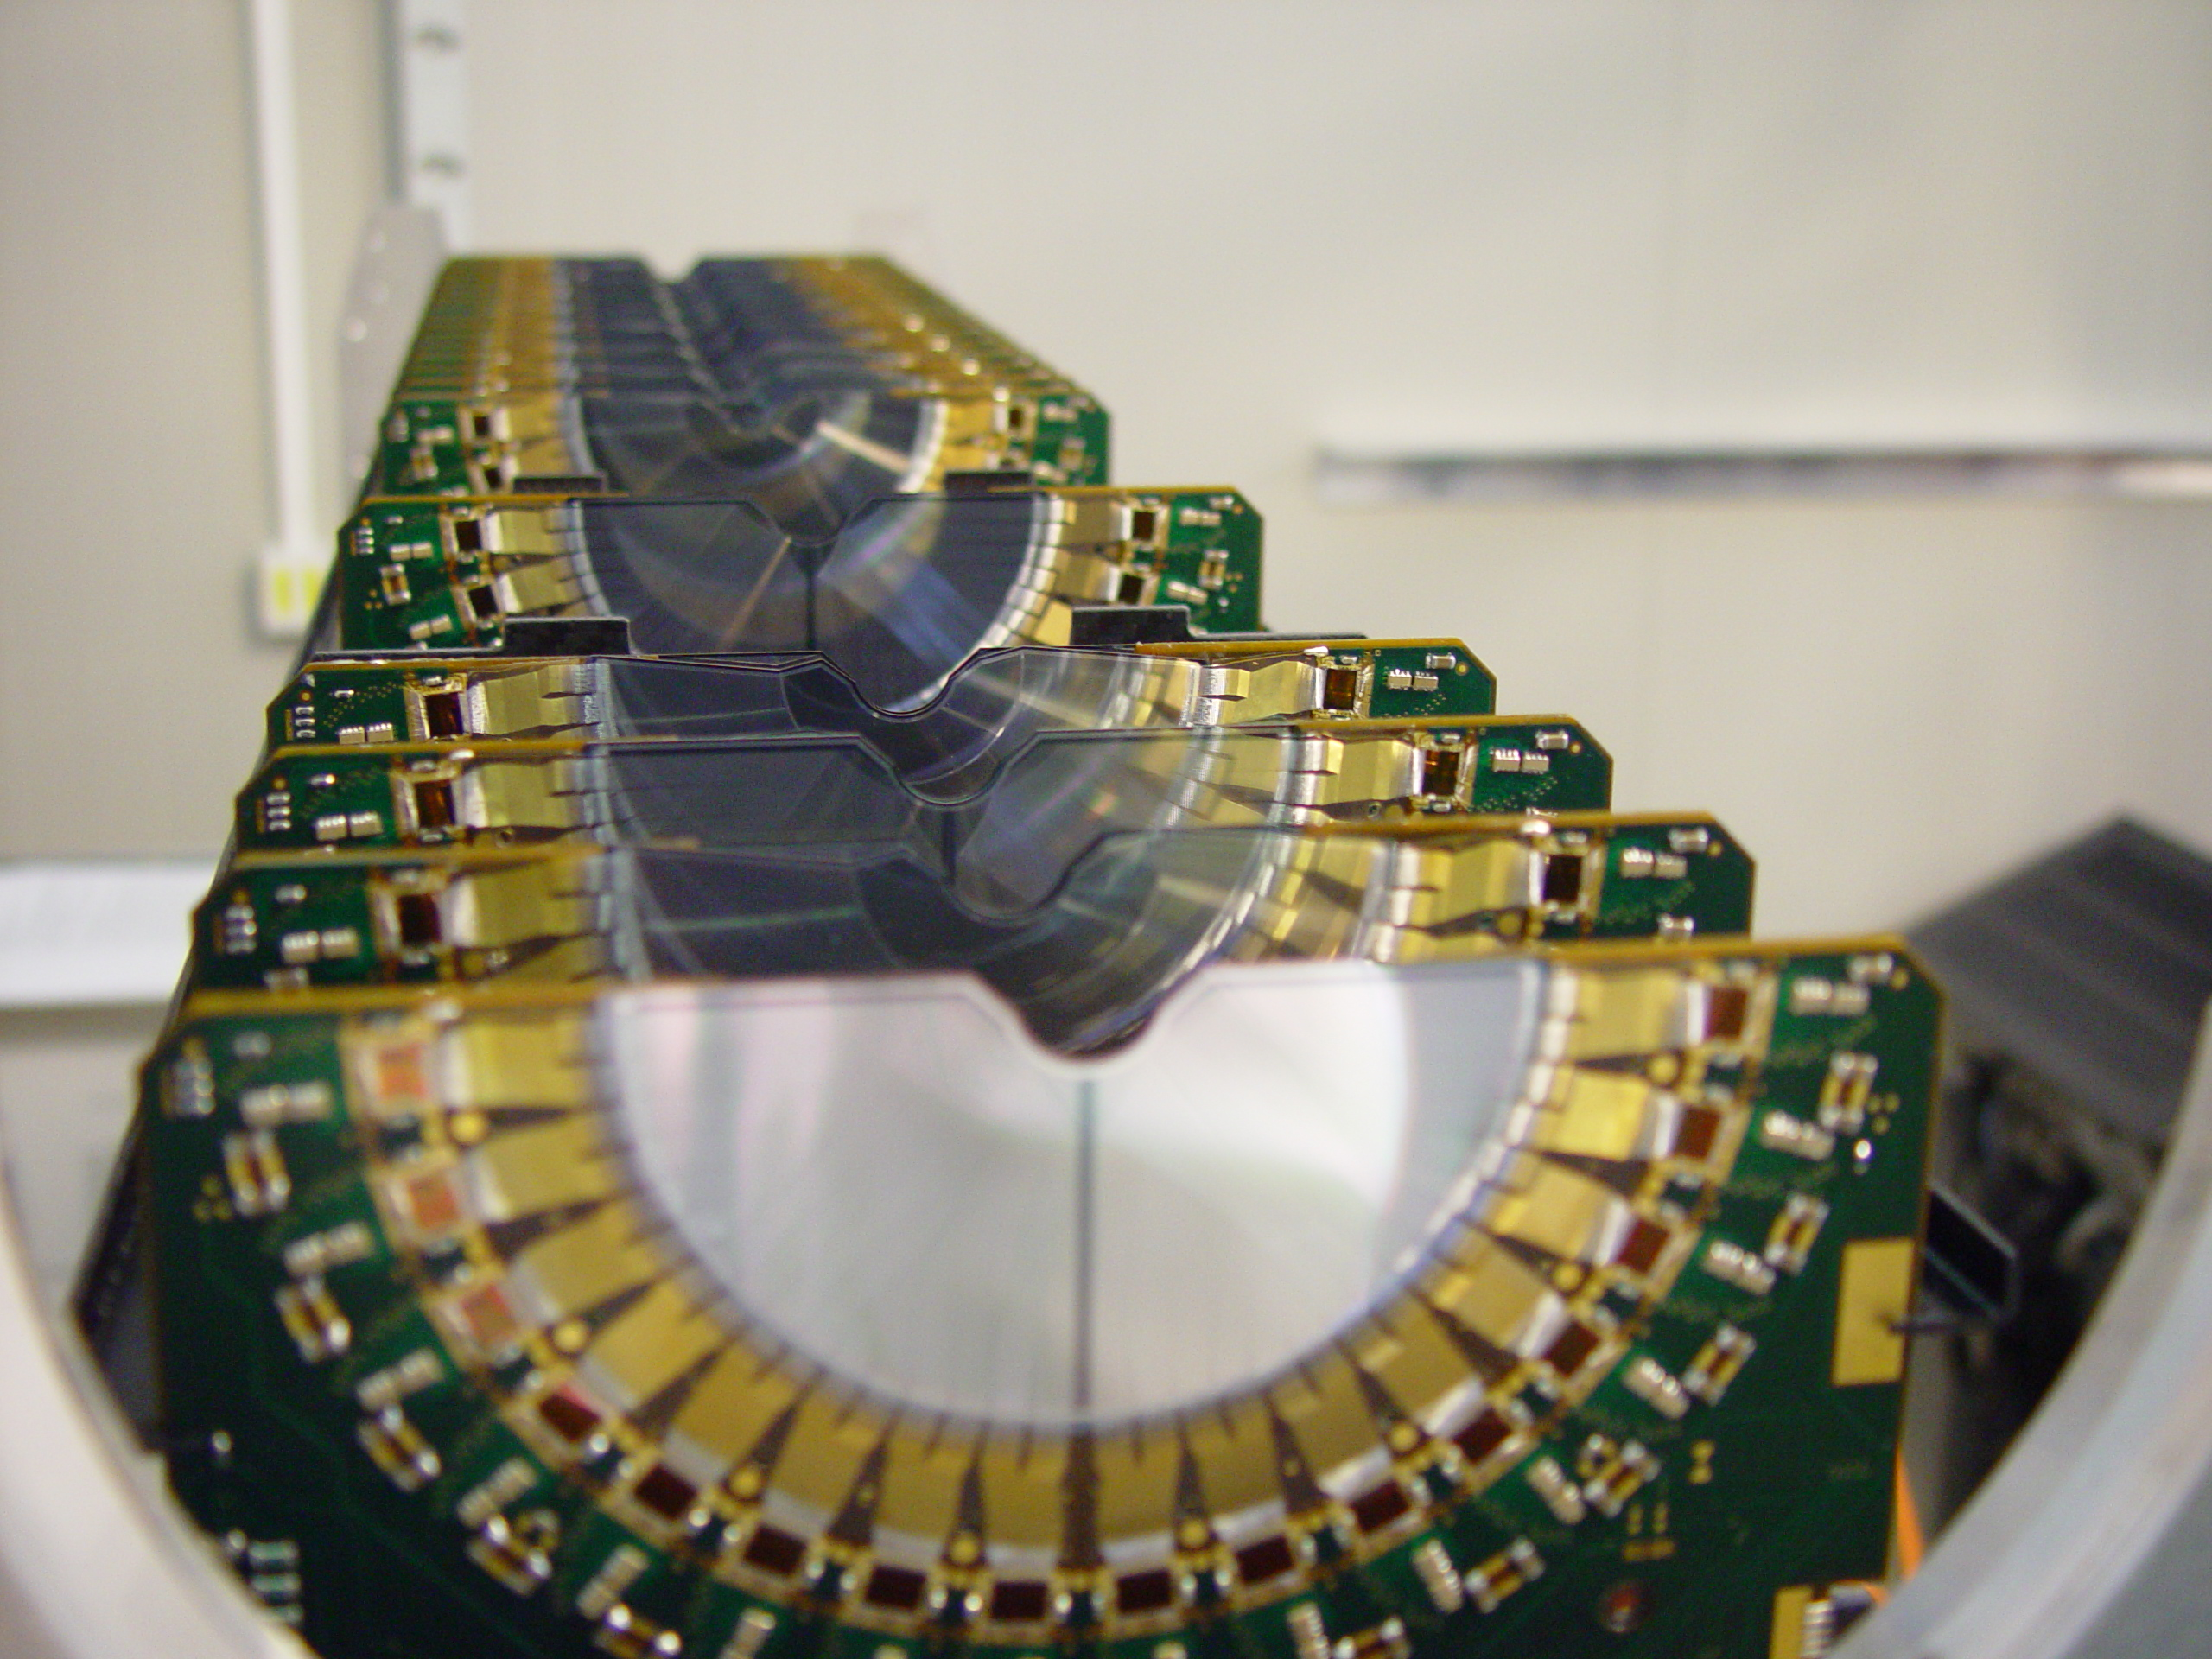
\includegraphics[height=3 cm]{Figures Introductory Lecture/LHCb Detector/LHCb_VELO.jpg}%source: http://cds.cern.ch/record/1017398
        \end{figure}
    \end{minipage}
    \vspace{-1cm}
    \begin{figure}[h]
    \centering
    \begin{overpic}[width=0.8\textwidth]{Figures Introductory Lecture/LHCb Detector/LHCb_1.png}
          
        \put (3,35) {\colorbox{LHCbDarkBlue!80}{\textcolor{LHCbLightBlue}{\centering \tiny  VELO}}}


   
    \end{overpic}
    \end{figure}
\end{frame}
\begin{frame}{Vertex Locator (VELO)} \centering
\begin{minipage}{.59\textwidth}
    \begin{itemize}
        \item Spurrekonstruktion
        \item Identifikation von Vertices

    \end{itemize}
\end{minipage}
\begin{minipage}{.39\textwidth}
  \rotatebox{180}{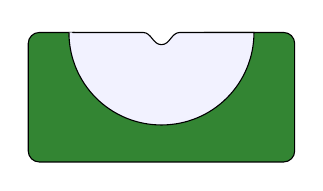
\begin{tikzpicture}[scale=.47]
        %Rand der Grafik
     \draw[rounded corners,cap=round,fill=green!40!black!80] (-3,-1)--(-3,-0)--(-1.5,0) -- (0,-1) -- (1.5,0) -- (4.2,0) -- (4.2,-3.5) -- (-3,-3.5) -- (-3,-1);
    % \draw[red] (-3,-2) circle (2pt){};

    % \draw[red] (-3,3) circle (2pt){};
    % \draw[red] (5,-2) circle (2pt){};
    % \draw[red] (5,3) circle (2pt){};
        \draw[cap=round,fill=blue!5] (-1.8,0) to  (0.1,0) to [out=0,in=180] (0.6,-0.33) to [out=0,in=180](1.1,0) to (3.1,0) [out=-90,in=0] to (0.6,-2.5) [out=180,in=-90] to (-1.9,0){};
            \draw  (-2.75,-0.12) node [right]{\textcolor{yellow!90!black!89!orange!90}{\rotatebox{0}{\scriptsize$\hrectangleblack$}}};
            \draw  (-2.71,-0.5) node [right]{\textcolor{yellow!90!black!89!orange!90}{\rotatebox{10}{\scriptsize$\hrectangleblack$}}};
            \draw  (-2.58,-0.94) node [right]{\textcolor{yellow!90!black!89!orange!90}{\rotatebox{20}{\scriptsize$\hrectangleblack$}}};
            \draw  (-2.38,-1.375) node [right]{\textcolor{yellow!90!black!89!orange!90}{\rotatebox{30}{\scriptsize$\hrectangleblack$}}};
            \draw  (-2.11,-1.76) node [right]{\textcolor{yellow!90!black!89!orange!90}{\rotatebox{40}{\scriptsize$\hrectangleblack$}}};
            \draw  (-1.76,-2.11) node [right]{\textcolor{yellow!90!black!89!orange!90}{\rotatebox{50}{\scriptsize$\hrectangleblack$}}};
            \draw  (-1.375,-2.38) node [right]{\textcolor{yellow!90!black!89!orange!90}{\rotatebox{60}{\scriptsize$\hrectangleblack$}}};
            \draw  (-0.94,-2.58) node [right]{\textcolor{yellow!90!black!89!orange!90}{\rotatebox{70}{\scriptsize$\hrectangleblack$}}};
            \draw  (-0.48,-2.71) node [right]{\textcolor{yellow!90!black!89!orange!90}{\rotatebox{80}{\scriptsize$\hrectangleblack$}}};
            \draw  (0.05,-2.75) node [right]{\textcolor{yellow!90!black!89!orange!90}{\rotatebox{90}{\scriptsize$\hrectangleblack$}}};
            \draw  (0.48,-2.71) node [right]{\textcolor{yellow!90!black!89!orange!90}{\rotatebox{100}{\scriptsize$\hrectangleblack$}}};
            \draw  (0.94,-2.58) node [right]{\textcolor{yellow!90!black!89!orange!90}{\rotatebox{110}{\scriptsize$\hrectangleblack$}}};
            \draw  (1.375,-2.38) node [right]{\textcolor{yellow!90!black!89!orange!90}{\rotatebox{120}{\scriptsize$\hrectangleblack$}}};
            \draw  (1.76,-2.11) node [right]{\textcolor{yellow!90!black!89!orange!90}{\rotatebox{130}{\scriptsize$\hrectangleblack$}}};
            \draw  (2.11,-1.76) node [right]{\textcolor{yellow!90!black!89!orange!90}{\rotatebox{140}{\scriptsize$\hrectangleblack$}}};
            \draw  (2.38,-1.375) node [right]{\textcolor{yellow!90!black!89!orange!90}{\rotatebox{150}{\scriptsize$\hrectangleblack$}}};
            \draw  (2.58,-0.94) node [right]{\textcolor{yellow!90!black!89!orange!90}{\rotatebox{160}{\scriptsize$\hrectangleblack$}}};
            \draw  (2.71,-0.5) node [right]{\textcolor{yellow!90!black!89!orange!90}{\rotatebox{170}{\scriptsize$\hrectangleblack$}}};
            \draw  (2.75,-0.12) node [right]{\textcolor{yellow!90!black!89!orange!90}{\rotatebox{180}{\scriptsize$\hrectangleblack$}}};
    \end{tikzpicture}} \\\vspace{-8pt}\\ 
    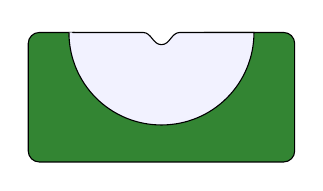
\begin{tikzpicture}[scale=.47]
        %Rand der Grafik
     \draw[rounded corners,cap=round,fill=green!40!black!80] (-3,-1)--(-3,-0)--(-1.5,0) -- (0,-1) -- (1.5,0) -- (4.2,0) -- (4.2,-3.5) -- (-3,-3.5) -- (-3,-1);
    % \draw[red] (-3,-2) circle (2pt){};

    % \draw[red] (-3,3) circle (2pt){};
    % \draw[red] (5,-2) circle (2pt){};
    % \draw[red] (5,3) circle (2pt){};
        \draw[cap=round,fill=blue!5] (-1.8,0) to  (0.1,0) to [out=0,in=180] (0.6,-0.33) to [out=0,in=180](1.1,0) to (3.1,0) [out=-90,in=0] to (0.6,-2.5) [out=180,in=-90] to (-1.9,0){};
            \draw  (-2.75,-0.12) node [right]{\textcolor{yellow!90!black!89!orange!90}{\rotatebox{0}{\scriptsize$\hrectangleblack$}}};
            \draw  (-2.71,-0.5) node [right]{\textcolor{yellow!90!black!89!orange!90}{\rotatebox{10}{\scriptsize$\hrectangleblack$}}};
            \draw  (-2.58,-0.94) node [right]{\textcolor{yellow!90!black!89!orange!90}{\rotatebox{20}{\scriptsize$\hrectangleblack$}}};
            \draw  (-2.38,-1.375) node [right]{\textcolor{yellow!90!black!89!orange!90}{\rotatebox{30}{\scriptsize$\hrectangleblack$}}};
            \draw  (-2.11,-1.76) node [right]{\textcolor{yellow!90!black!89!orange!90}{\rotatebox{40}{\scriptsize$\hrectangleblack$}}};
            \draw  (-1.76,-2.11) node [right]{\textcolor{yellow!90!black!89!orange!90}{\rotatebox{50}{\scriptsize$\hrectangleblack$}}};
            \draw  (-1.375,-2.38) node [right]{\textcolor{yellow!90!black!89!orange!90}{\rotatebox{60}{\scriptsize$\hrectangleblack$}}};
            \draw  (-0.94,-2.58) node [right]{\textcolor{yellow!90!black!89!orange!90}{\rotatebox{70}{\scriptsize$\hrectangleblack$}}};
            \draw  (-0.48,-2.71) node [right]{\textcolor{yellow!90!black!89!orange!90}{\rotatebox{80}{\scriptsize$\hrectangleblack$}}};
            \draw  (0.05,-2.75) node [right]{\textcolor{yellow!90!black!89!orange!90}{\rotatebox{90}{\scriptsize$\hrectangleblack$}}};
            \draw  (0.48,-2.71) node [right]{\textcolor{yellow!90!black!89!orange!90}{\rotatebox{100}{\scriptsize$\hrectangleblack$}}};
            \draw  (0.94,-2.58) node [right]{\textcolor{yellow!90!black!89!orange!90}{\rotatebox{110}{\scriptsize$\hrectangleblack$}}};
            \draw  (1.375,-2.38) node [right]{\textcolor{yellow!90!black!89!orange!90}{\rotatebox{120}{\scriptsize$\hrectangleblack$}}};
            \draw  (1.76,-2.11) node [right]{\textcolor{yellow!90!black!89!orange!90}{\rotatebox{130}{\scriptsize$\hrectangleblack$}}};
            \draw  (2.11,-1.76) node [right]{\textcolor{yellow!90!black!89!orange!90}{\rotatebox{140}{\scriptsize$\hrectangleblack$}}};
            \draw  (2.38,-1.375) node [right]{\textcolor{yellow!90!black!89!orange!90}{\rotatebox{150}{\scriptsize$\hrectangleblack$}}};
            \draw  (2.58,-0.94) node [right]{\textcolor{yellow!90!black!89!orange!90}{\rotatebox{160}{\scriptsize$\hrectangleblack$}}};
            \draw  (2.71,-0.5) node [right]{\textcolor{yellow!90!black!89!orange!90}{\rotatebox{170}{\scriptsize$\hrectangleblack$}}};
            \draw  (2.75,-0.12) node [right]{\textcolor{yellow!90!black!89!orange!90}{\rotatebox{180}{\scriptsize$\hrectangleblack$}}};
    \end{tikzpicture}\end{minipage}
    \begin{tikzpicture}[scale=1.2]
    %Rand der Grafik
    \draw[white] (-3,-1.5) circle (2pt){};
    \draw[white] (-3,2.5) circle (2pt){};
    \draw[white] (5,-1.5) circle (2pt){};
    \draw[white] (5,2.5) circle (2pt){};

%VELO stations
%below beam
    \draw[--,line width=1.5pt,green!40!black!80] (0.05,-0.25) --++ (0,.75){};
    \draw[--,line width=1.5pt,green!40!black!80] (0.25,-0.25) --++ (0,.75){};
    \draw[--,line width=1.5pt,green!40!black!80] (0.45,-0.25) --++ (0,.75){};
    \draw[--,line width=1.5pt,green!40!black!80] (0.65,-0.25) --++ (0,.75){};
    \draw[--,line width=1.5pt,green!40!black!80] (0.85,-0.25) --++ (0,.75){};
    \draw[--,line width=1.5pt,green!40!black!80] (1.05,-0.25) --++ (0,.75){};
     \draw[--,line width=1.5pt,green!40!black!80] (1.25,-0.25) --++ (0,.75){};
    \draw[--,line width=1.5pt,green!40!black!80] (1.45,-0.25) --++ (0,.75){};
    \draw[--,line width=1.5pt,green!40!black!80] (1.65,-0.25) --++ (0,.75){};
    \draw[--,line width=1.5pt,green!40!black!80] (1.85,-0.25) --++ (0,.75){};
    \draw[--,line width=1.5pt,green!40!black!80] (2.05,-0.25) --++ (0,.75){};
       
        \draw[--,line width=1.5pt,green!40!black!80] (2.55,-0.25) --++ (0,.75){};
        \draw[--,line width=1.5pt,green!40!black!80] (3.05,-0.25) --++ (0,.75){};
        \draw[--,line width=1.5pt,green!40!black!80] (3.55,-0.25) --++ (0,.75){};

        \draw[--,line width=1.5pt,green!40!black!80] (4.25,-0.25) --++ (0,.75){};
        \draw[--,line width=1.5pt,green!40!black!80] (4.45,-0.25) --++ (0,.75){};                
        \draw[--,line width=1.5pt,green!40!black!80] (4.65,-0.25) --++ (0,.75){};
        \draw[--,line width=1.5pt,green!40!black!80] (4.85,-0.25) --++ (0,.75){};
        
    \draw[--,line width=1.5pt,green!40!black!80] (-0.2,-0.25) --++ (0,.75){};
    \draw[--,line width=1.5pt,green!40!black!80] (-0.4,-0.25) --++ (0,.75){};
    \draw[--,line width=1.5pt,green!40!black!80] (-0.6,-0.25) --++ (0,.75){};
    \draw[--,line width=1.5pt,green!40!black!80] (-0.8,-0.25) --++ (0,.75){};
    \draw[--,line width=1.5pt,green!40!black!80] (-1.4,-0.25) --++ (0,.75){};
    \draw[--,line width=1.5pt,green!40!black!80] (-2,-0.25) --++ (0,.75){};
    \draw[--,line width=1.5pt,green!40!black!80] (-2.2,-0.25) --++ (0,.75){};
    \draw[--,line width=1.5pt,green!40!black!80] (-2.4,-0.25) --++ (0,.75){};
    \draw[--,line width=1.5pt,green!40!black!80] (-2.6,-0.25) --++ (0,.75){};
%above beam
    \draw[--,line width=1.5pt,green!40!black!80] (0,1) --++ (0,.75){};
    \draw[--,line width=1.5pt,green!40!black!80] (0.2,1) --++ (0,.75){};
    \draw[--,line width=1.5pt,green!40!black!80] (0.4,1) --++ (0,.75){};
    \draw[--,line width=1.5pt,green!40!black!80] (0.6,1) --++ (0,.75){};
    \draw[--,line width=1.5pt,green!40!black!80] (0.8,1) --++ (0,.75){};
    \draw[--,line width=1.5pt,green!40!black!80] (1,1) --++ (0,.75){};
     \draw[--,line width=1.5pt,green!40!black!80] (1.2,1) --++ (0,.75){};
    \draw[--,line width=1.5pt,green!40!black!80] (1.4,1) --++ (0,.75){};
    \draw[--,line width=1.5pt,green!40!black!80] (1.6,1) --++ (0,.75){};
    \draw[--,line width=1.5pt,green!40!black!80] (1.8,1) --++ (0,.75){};
    \draw[--,line width=1.5pt,green!40!black!80] (2,1) --++ (0,.75){};
       
        \draw[--,line width=1.5pt,green!40!black!80] (2.5,1) --++ (0,.75){};
        \draw[--,line width=1.5pt,green!40!black!80] (3,1) --++ (0,.75){};
        \draw[--,line width=1.5pt,green!40!black!80] (3.5,1) --++ (0,.75){};

        \draw[--,line width=1.5pt,green!40!black!80] (4.2,1) --++ (0,.75){};
        \draw[--,line width=1.5pt,green!40!black!80] (4.4,1) --++ (0,.75){};                
        \draw[--,line width=1.5pt,green!40!black!80] (4.6,1) --++ (0,.75){};
        \draw[--,line width=1.5pt,green!40!black!80] (4.8,1) --++ (0,.75){};
        
    \draw[--,line width=1.5pt,green!40!black!80] (-0.2,1) --++ (0,.75){};
    \draw[--,line width=1.5pt,green!40!black!80] (-0.4,1) --++ (0,.75){};
    \draw[--,line width=1.5pt,green!40!black!80] (-0.6,1) --++ (0,.75){};
    \draw[--,line width=1.5pt,green!40!black!80] (-0.8,1) --++ (0,.75){};
    \draw[--,line width=1.5pt,green!40!black!80] (-1.4,1) --++ (0,.75){};
    \draw[--,line width=1.5pt,green!40!black!80] (-2,1) --++ (0,.75){};
    \draw[--,line width=1.5pt,green!40!black!80] (-2.2,1) --++ (0,.75){};
    \draw[--,line width=1.5pt,green!40!black!80] (-2.4,1) --++ (0,.75){};
    \draw[--,line width=1.5pt,green!40!black!80] (-2.6,1) --++ (0,.75){};
%pp
\draw[->,line width=2pt](-0.5,.75) node [left] {$p$}--++ (0.5,0){};
\draw[->,line width=2pt](0.5,.75) node [right] {$p$}--++ (-0.5,0){};

%Labels 
\midlabelline{-3,-0.25}{-3,1.75}{\scriptsize\SI{6,6}{\centi\metre}}
\midlabelline{-2.6,-0.75}{4.9,-.75}{\scriptsize\SI{1}{\metre}}

% %Events 
% \node at (0.2,1) {\textcolor{red}{\scriptsize$\mathbf{\times}$}};
% \node at (0.4,1.2) {\textcolor{red}{\scriptsize$\mathbf{\times}$}};
% \node at (0.6,1.4) {\textcolor{red}{\scriptsize$\mathbf{\times}$}};
% \node at (0.8,1.6) {\textcolor{red}{\scriptsize$\mathbf{\times}$}};


% \node at (0.65,0.425) {\textcolor{red}{\scriptsize$\mathbf{\times}$}};
% \node at (0.85,0.325) {\textcolor{red}{\scriptsize$\mathbf{\times}$}};
% \node at (1.05,0.225) {\textcolor{red}{\scriptsize$\mathbf{\times}$}};

% \node at (1.25,0.08) {\textcolor{red}{\scriptsize$\mathbf{\times}$}};
% \node at (1.25,0.2) {\textcolor{red}{\scriptsize$\mathbf{\times}$}};

% \node at (1.45,-0.08) {\textcolor{red}{\scriptsize$\mathbf{\times}$}};
% \node at (1.45,0.2) {\textcolor{red}{\scriptsize$\mathbf{\times}$}};

% \node at (1.65,-0.24) {\textcolor{red}{\scriptsize$\mathbf{\times}$}};
% \node at (1.65,0.2) {\textcolor{red}{\scriptsize$\mathbf{\times}$}};

% \node at (1.85,0.2) {\textcolor{red}{\scriptsize$\mathbf{\times}$}};
% \node at (2.05,0.2) {\textcolor{red}{\scriptsize$\mathbf{\times}$}};
% \node at (2.55,0.2) {\textcolor{red}{\scriptsize$\mathbf{\times}$}};
% \node at (3.05,0.2) {\textcolor{red}{\scriptsize$\mathbf{\times}$}};
% \node at (3.55,0.2) {\textcolor{red}{\scriptsize$\mathbf{\times}$}};
% \node at (4.25,0.2) {\textcolor{red}{\scriptsize$\mathbf{\times}$}};
% \node at (4.45,0.4) {\textcolor{red}{\scriptsize$\mathbf{\times}$}};
% \node at (4.6,1.1) {\textcolor{red}{\scriptsize$\mathbf{\times}$}};
% \node at (4.8,1.7) {\textcolor{red}{\scriptsize$\mathbf{\times}$}};

% %Funktion

% \draw[ rounded corners,cap=round,--,red!black!49,line width=2pt] (0,.8) -- (1.1,1.85){};
% \draw[ rounded corners,cap=round,--,red,line width=2pt] (0,.75) -- (1.1,0.2){};
% \draw[ rounded corners,cap=round,--,red,line width=2pt] (2,-0.52) -- (1.1,0.2){};
% \draw[ rounded corners,cap=round,--,red,line width=2pt] (4.38,0.2) -- (1.1,0.2){};
% \draw[ rounded corners,cap=round,--,red,line width=2pt] (4.38,0.2) -- (4.95,2.3){};
% \draw[ rounded corners,cap=round,--,red,line width=1pt,dashed] (4.38,0.2) -- (4.8,-0.3) node [right]{?};
    \end{tikzpicture}
\end{frame}
\begin{frame}{Vertex Locator (VELO)} \centering\addtocounter{framenumber}{-1}
\begin{minipage}{.59\textwidth}
    \begin{itemize}
        \item Spurrekonstruktion
        \item Identifikation von Vertices

    \end{itemize}
\end{minipage}
\begin{minipage}{.39\textwidth}
  \rotatebox{180}{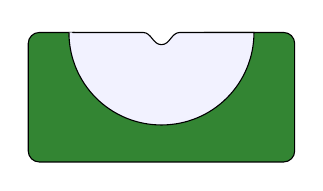
\begin{tikzpicture}[scale=.47]
        %Rand der Grafik
     \draw[rounded corners,cap=round,fill=green!40!black!80] (-3,-1)--(-3,-0)--(-1.5,0) -- (0,-1) -- (1.5,0) -- (4.2,0) -- (4.2,-3.5) -- (-3,-3.5) -- (-3,-1);
    % \draw[red] (-3,-2) circle (2pt){};

    % \draw[red] (-3,3) circle (2pt){};
    % \draw[red] (5,-2) circle (2pt){};
    % \draw[red] (5,3) circle (2pt){};
        \draw[cap=round,fill=blue!5] (-1.8,0) to  (0.1,0) to [out=0,in=180] (0.6,-0.33) to [out=0,in=180](1.1,0) to (3.1,0) [out=-90,in=0] to (0.6,-2.5) [out=180,in=-90] to (-1.9,0){};
            \draw  (-2.75,-0.12) node [right]{\textcolor{yellow!90!black!89!orange!90}{\rotatebox{0}{\scriptsize$\hrectangleblack$}}};
            \draw  (-2.71,-0.5) node [right]{\textcolor{yellow!90!black!89!orange!90}{\rotatebox{10}{\scriptsize$\hrectangleblack$}}};
            \draw  (-2.58,-0.94) node [right]{\textcolor{yellow!90!black!89!orange!90}{\rotatebox{20}{\scriptsize$\hrectangleblack$}}};
            \draw  (-2.38,-1.375) node [right]{\textcolor{yellow!90!black!89!orange!90}{\rotatebox{30}{\scriptsize$\hrectangleblack$}}};
            \draw  (-2.11,-1.76) node [right]{\textcolor{yellow!90!black!89!orange!90}{\rotatebox{40}{\scriptsize$\hrectangleblack$}}};
            \draw  (-1.76,-2.11) node [right]{\textcolor{yellow!90!black!89!orange!90}{\rotatebox{50}{\scriptsize$\hrectangleblack$}}};
            \draw  (-1.375,-2.38) node [right]{\textcolor{yellow!90!black!89!orange!90}{\rotatebox{60}{\scriptsize$\hrectangleblack$}}};
            \draw  (-0.94,-2.58) node [right]{\textcolor{yellow!90!black!89!orange!90}{\rotatebox{70}{\scriptsize$\hrectangleblack$}}};
            \draw  (-0.48,-2.71) node [right]{\textcolor{yellow!90!black!89!orange!90}{\rotatebox{80}{\scriptsize$\hrectangleblack$}}};
            \draw  (0.05,-2.75) node [right]{\textcolor{yellow!90!black!89!orange!90}{\rotatebox{90}{\scriptsize$\hrectangleblack$}}};
            \draw  (0.48,-2.71) node [right]{\textcolor{yellow!90!black!89!orange!90}{\rotatebox{100}{\scriptsize$\hrectangleblack$}}};
            \draw  (0.94,-2.58) node [right]{\textcolor{yellow!90!black!89!orange!90}{\rotatebox{110}{\scriptsize$\hrectangleblack$}}};
            \draw  (1.375,-2.38) node [right]{\textcolor{yellow!90!black!89!orange!90}{\rotatebox{120}{\scriptsize$\hrectangleblack$}}};
            \draw  (1.76,-2.11) node [right]{\textcolor{yellow!90!black!89!orange!90}{\rotatebox{130}{\scriptsize$\hrectangleblack$}}};
            \draw  (2.11,-1.76) node [right]{\textcolor{yellow!90!black!89!orange!90}{\rotatebox{140}{\scriptsize$\hrectangleblack$}}};
            \draw  (2.38,-1.375) node [right]{\textcolor{yellow!90!black!89!orange!90}{\rotatebox{150}{\scriptsize$\hrectangleblack$}}};
            \draw  (2.58,-0.94) node [right]{\textcolor{yellow!90!black!89!orange!90}{\rotatebox{160}{\scriptsize$\hrectangleblack$}}};
            \draw  (2.71,-0.5) node [right]{\textcolor{yellow!90!black!89!orange!90}{\rotatebox{170}{\scriptsize$\hrectangleblack$}}};
            \draw  (2.75,-0.12) node [right]{\textcolor{yellow!90!black!89!orange!90}{\rotatebox{180}{\scriptsize$\hrectangleblack$}}};
    \end{tikzpicture}} \\\vspace{-8pt}\\ 
    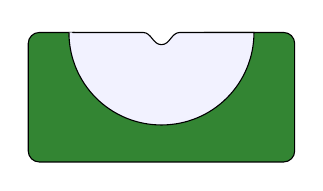
\begin{tikzpicture}[scale=.47]
        %Rand der Grafik
     \draw[rounded corners,cap=round,fill=green!40!black!80] (-3,-1)--(-3,-0)--(-1.5,0) -- (0,-1) -- (1.5,0) -- (4.2,0) -- (4.2,-3.5) -- (-3,-3.5) -- (-3,-1);
    % \draw[red] (-3,-2) circle (2pt){};

    % \draw[red] (-3,3) circle (2pt){};
    % \draw[red] (5,-2) circle (2pt){};
    % \draw[red] (5,3) circle (2pt){};
        \draw[cap=round,fill=blue!5] (-1.8,0) to  (0.1,0) to [out=0,in=180] (0.6,-0.33) to [out=0,in=180](1.1,0) to (3.1,0) [out=-90,in=0] to (0.6,-2.5) [out=180,in=-90] to (-1.9,0){};
            \draw  (-2.75,-0.12) node [right]{\textcolor{yellow!90!black!89!orange!90}{\rotatebox{0}{\scriptsize$\hrectangleblack$}}};
            \draw  (-2.71,-0.5) node [right]{\textcolor{yellow!90!black!89!orange!90}{\rotatebox{10}{\scriptsize$\hrectangleblack$}}};
            \draw  (-2.58,-0.94) node [right]{\textcolor{yellow!90!black!89!orange!90}{\rotatebox{20}{\scriptsize$\hrectangleblack$}}};
            \draw  (-2.38,-1.375) node [right]{\textcolor{yellow!90!black!89!orange!90}{\rotatebox{30}{\scriptsize$\hrectangleblack$}}};
            \draw  (-2.11,-1.76) node [right]{\textcolor{yellow!90!black!89!orange!90}{\rotatebox{40}{\scriptsize$\hrectangleblack$}}};
            \draw  (-1.76,-2.11) node [right]{\textcolor{yellow!90!black!89!orange!90}{\rotatebox{50}{\scriptsize$\hrectangleblack$}}};
            \draw  (-1.375,-2.38) node [right]{\textcolor{yellow!90!black!89!orange!90}{\rotatebox{60}{\scriptsize$\hrectangleblack$}}};
            \draw  (-0.94,-2.58) node [right]{\textcolor{yellow!90!black!89!orange!90}{\rotatebox{70}{\scriptsize$\hrectangleblack$}}};
            \draw  (-0.48,-2.71) node [right]{\textcolor{yellow!90!black!89!orange!90}{\rotatebox{80}{\scriptsize$\hrectangleblack$}}};
            \draw  (0.05,-2.75) node [right]{\textcolor{yellow!90!black!89!orange!90}{\rotatebox{90}{\scriptsize$\hrectangleblack$}}};
            \draw  (0.48,-2.71) node [right]{\textcolor{yellow!90!black!89!orange!90}{\rotatebox{100}{\scriptsize$\hrectangleblack$}}};
            \draw  (0.94,-2.58) node [right]{\textcolor{yellow!90!black!89!orange!90}{\rotatebox{110}{\scriptsize$\hrectangleblack$}}};
            \draw  (1.375,-2.38) node [right]{\textcolor{yellow!90!black!89!orange!90}{\rotatebox{120}{\scriptsize$\hrectangleblack$}}};
            \draw  (1.76,-2.11) node [right]{\textcolor{yellow!90!black!89!orange!90}{\rotatebox{130}{\scriptsize$\hrectangleblack$}}};
            \draw  (2.11,-1.76) node [right]{\textcolor{yellow!90!black!89!orange!90}{\rotatebox{140}{\scriptsize$\hrectangleblack$}}};
            \draw  (2.38,-1.375) node [right]{\textcolor{yellow!90!black!89!orange!90}{\rotatebox{150}{\scriptsize$\hrectangleblack$}}};
            \draw  (2.58,-0.94) node [right]{\textcolor{yellow!90!black!89!orange!90}{\rotatebox{160}{\scriptsize$\hrectangleblack$}}};
            \draw  (2.71,-0.5) node [right]{\textcolor{yellow!90!black!89!orange!90}{\rotatebox{170}{\scriptsize$\hrectangleblack$}}};
            \draw  (2.75,-0.12) node [right]{\textcolor{yellow!90!black!89!orange!90}{\rotatebox{180}{\scriptsize$\hrectangleblack$}}};
    \end{tikzpicture}\end{minipage}
    \begin{tikzpicture}[scale=1.2]
    %Rand der Grafik
    \draw[white] (-3,-1.5) circle (2pt){};
    \draw[white] (-3,2.5) circle (2pt){};
    \draw[white] (5,-1.5) circle (2pt){};
    \draw[white] (5,2.5) circle (2pt){};

%VELO stations
%below beam
    \draw[--,line width=1.5pt,green!40!black!80] (0.05,-0.25) --++ (0,.75){};
    \draw[--,line width=1.5pt,green!40!black!80] (0.25,-0.25) --++ (0,.75){};
    \draw[--,line width=1.5pt,green!40!black!80] (0.45,-0.25) --++ (0,.75){};
    \draw[--,line width=1.5pt,green!40!black!80] (0.65,-0.25) --++ (0,.75){};
    \draw[--,line width=1.5pt,green!40!black!80] (0.85,-0.25) --++ (0,.75){};
    \draw[--,line width=1.5pt,green!40!black!80] (1.05,-0.25) --++ (0,.75){};
     \draw[--,line width=1.5pt,green!40!black!80] (1.25,-0.25) --++ (0,.75){};
    \draw[--,line width=1.5pt,green!40!black!80] (1.45,-0.25) --++ (0,.75){};
    \draw[--,line width=1.5pt,green!40!black!80] (1.65,-0.25) --++ (0,.75){};
    \draw[--,line width=1.5pt,green!40!black!80] (1.85,-0.25) --++ (0,.75){};
    \draw[--,line width=1.5pt,green!40!black!80] (2.05,-0.25) --++ (0,.75){};
       
        \draw[--,line width=1.5pt,green!40!black!80] (2.55,-0.25) --++ (0,.75){};
        \draw[--,line width=1.5pt,green!40!black!80] (3.05,-0.25) --++ (0,.75){};
        \draw[--,line width=1.5pt,green!40!black!80] (3.55,-0.25) --++ (0,.75){};

        \draw[--,line width=1.5pt,green!40!black!80] (4.25,-0.25) --++ (0,.75){};
        \draw[--,line width=1.5pt,green!40!black!80] (4.45,-0.25) --++ (0,.75){};                
        \draw[--,line width=1.5pt,green!40!black!80] (4.65,-0.25) --++ (0,.75){};
        \draw[--,line width=1.5pt,green!40!black!80] (4.85,-0.25) --++ (0,.75){};
        
    \draw[--,line width=1.5pt,green!40!black!80] (-0.2,-0.25) --++ (0,.75){};
    \draw[--,line width=1.5pt,green!40!black!80] (-0.4,-0.25) --++ (0,.75){};
    \draw[--,line width=1.5pt,green!40!black!80] (-0.6,-0.25) --++ (0,.75){};
    \draw[--,line width=1.5pt,green!40!black!80] (-0.8,-0.25) --++ (0,.75){};
    \draw[--,line width=1.5pt,green!40!black!80] (-1.4,-0.25) --++ (0,.75){};
    \draw[--,line width=1.5pt,green!40!black!80] (-2,-0.25) --++ (0,.75){};
    \draw[--,line width=1.5pt,green!40!black!80] (-2.2,-0.25) --++ (0,.75){};
    \draw[--,line width=1.5pt,green!40!black!80] (-2.4,-0.25) --++ (0,.75){};
    \draw[--,line width=1.5pt,green!40!black!80] (-2.6,-0.25) --++ (0,.75){};
%above beam
    \draw[--,line width=1.5pt,green!40!black!80] (0,1) --++ (0,.75){};
    \draw[--,line width=1.5pt,green!40!black!80] (0.2,1) --++ (0,.75){};
    \draw[--,line width=1.5pt,green!40!black!80] (0.4,1) --++ (0,.75){};
    \draw[--,line width=1.5pt,green!40!black!80] (0.6,1) --++ (0,.75){};
    \draw[--,line width=1.5pt,green!40!black!80] (0.8,1) --++ (0,.75){};
    \draw[--,line width=1.5pt,green!40!black!80] (1,1) --++ (0,.75){};
     \draw[--,line width=1.5pt,green!40!black!80] (1.2,1) --++ (0,.75){};
    \draw[--,line width=1.5pt,green!40!black!80] (1.4,1) --++ (0,.75){};
    \draw[--,line width=1.5pt,green!40!black!80] (1.6,1) --++ (0,.75){};
    \draw[--,line width=1.5pt,green!40!black!80] (1.8,1) --++ (0,.75){};
    \draw[--,line width=1.5pt,green!40!black!80] (2,1) --++ (0,.75){};
       
        \draw[--,line width=1.5pt,green!40!black!80] (2.5,1) --++ (0,.75){};
        \draw[--,line width=1.5pt,green!40!black!80] (3,1) --++ (0,.75){};
        \draw[--,line width=1.5pt,green!40!black!80] (3.5,1) --++ (0,.75){};

        \draw[--,line width=1.5pt,green!40!black!80] (4.2,1) --++ (0,.75){};
        \draw[--,line width=1.5pt,green!40!black!80] (4.4,1) --++ (0,.75){};                
        \draw[--,line width=1.5pt,green!40!black!80] (4.6,1) --++ (0,.75){};
        \draw[--,line width=1.5pt,green!40!black!80] (4.8,1) --++ (0,.75){};
        
    \draw[--,line width=1.5pt,green!40!black!80] (-0.2,1) --++ (0,.75){};
    \draw[--,line width=1.5pt,green!40!black!80] (-0.4,1) --++ (0,.75){};
    \draw[--,line width=1.5pt,green!40!black!80] (-0.6,1) --++ (0,.75){};
    \draw[--,line width=1.5pt,green!40!black!80] (-0.8,1) --++ (0,.75){};
    \draw[--,line width=1.5pt,green!40!black!80] (-1.4,1) --++ (0,.75){};
    \draw[--,line width=1.5pt,green!40!black!80] (-2,1) --++ (0,.75){};
    \draw[--,line width=1.5pt,green!40!black!80] (-2.2,1) --++ (0,.75){};
    \draw[--,line width=1.5pt,green!40!black!80] (-2.4,1) --++ (0,.75){};
    \draw[--,line width=1.5pt,green!40!black!80] (-2.6,1) --++ (0,.75){};
%pp
\draw[->,line width=2pt](-0.5,.75) node [left] {$p$}--++ (0.5,0){};
\draw[->,line width=2pt](0.5,.75) node [right] {$p$}--++ (-0.5,0){};

%Labels 
\midlabelline{-3,-0.25}{-3,1.75}{\scriptsize\SI{6,6}{\centi\metre}}
\midlabelline{-2.6,-0.75}{4.9,-.75}{\scriptsize\SI{1}{\metre}}

%Events 
\node at (0.2,1) {\textcolor{red}{\scriptsize$\mathbf{\times}$}};
\node at (0.4,1.2) {\textcolor{red}{\scriptsize$\mathbf{\times}$}};
\node at (0.6,1.4) {\textcolor{red}{\scriptsize$\mathbf{\times}$}};
\node at (0.8,1.6) {\textcolor{red}{\scriptsize$\mathbf{\times}$}};


\node at (0.65,0.425) {\textcolor{red}{\scriptsize$\mathbf{\times}$}};
\node at (0.85,0.325) {\textcolor{red}{\scriptsize$\mathbf{\times}$}};
\node at (1.05,0.225) {\textcolor{red}{\scriptsize$\mathbf{\times}$}};

\node at (1.25,0.08) {\textcolor{red}{\scriptsize$\mathbf{\times}$}};
\node at (1.25,0.2) {\textcolor{red}{\scriptsize$\mathbf{\times}$}};

\node at (1.45,-0.08) {\textcolor{red}{\scriptsize$\mathbf{\times}$}};
\node at (1.45,0.2) {\textcolor{red}{\scriptsize$\mathbf{\times}$}};

\node at (1.65,-0.24) {\textcolor{red}{\scriptsize$\mathbf{\times}$}};
\node at (1.65,0.2) {\textcolor{red}{\scriptsize$\mathbf{\times}$}};

\node at (1.85,0.2) {\textcolor{red}{\scriptsize$\mathbf{\times}$}};
\node at (2.05,0.2) {\textcolor{red}{\scriptsize$\mathbf{\times}$}};
\node at (2.55,0.2) {\textcolor{red}{\scriptsize$\mathbf{\times}$}};
\node at (3.05,0.2) {\textcolor{red}{\scriptsize$\mathbf{\times}$}};
\node at (3.55,0.2) {\textcolor{red}{\scriptsize$\mathbf{\times}$}};
\node at (4.25,0.2) {\textcolor{red}{\scriptsize$\mathbf{\times}$}};
\node at (4.45,0.4) {\textcolor{red}{\scriptsize$\mathbf{\times}$}};
\node at (4.6,1.1) {\textcolor{red}{\scriptsize$\mathbf{\times}$}};
\node at (4.8,1.7) {\textcolor{red}{\scriptsize$\mathbf{\times}$}};

% %Funktion

% \draw[ rounded corners,cap=round,--,red!black!49,line width=2pt] (0,.8) -- (1.1,1.85){};
% \draw[ rounded corners,cap=round,--,red,line width=2pt] (0,.75) -- (1.1,0.2){};
% \draw[ rounded corners,cap=round,--,red,line width=2pt] (2,-0.52) -- (1.1,0.2){};
% \draw[ rounded corners,cap=round,--,red,line width=2pt] (4.38,0.2) -- (1.1,0.2){};
% \draw[ rounded corners,cap=round,--,red,line width=2pt] (4.38,0.2) -- (4.95,2.3){};
% \draw[ rounded corners,cap=round,--,red,line width=1pt,dashed] (4.38,0.2) -- (4.8,-0.3) node [right]{?};
    \end{tikzpicture}
\end{frame}
\begin{frame}{Vertex Locator (VELO)} \centering\addtocounter{framenumber}{-1}
\begin{minipage}{.59\textwidth}
    \begin{itemize}
        \item Spurrekonstruktion
        \item Identifikation von Vertices

    \end{itemize}
\end{minipage}
\begin{minipage}{.39\textwidth}
  \rotatebox{180}{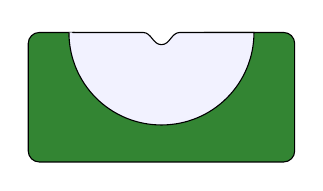
\begin{tikzpicture}[scale=.47]
        %Rand der Grafik
     \draw[rounded corners,cap=round,fill=green!40!black!80] (-3,-1)--(-3,-0)--(-1.5,0) -- (0,-1) -- (1.5,0) -- (4.2,0) -- (4.2,-3.5) -- (-3,-3.5) -- (-3,-1);
    % \draw[red] (-3,-2) circle (2pt){};

    % \draw[red] (-3,3) circle (2pt){};
    % \draw[red] (5,-2) circle (2pt){};
    % \draw[red] (5,3) circle (2pt){};
        \draw[cap=round,fill=blue!5] (-1.8,0) to  (0.1,0) to [out=0,in=180] (0.6,-0.33) to [out=0,in=180](1.1,0) to (3.1,0) [out=-90,in=0] to (0.6,-2.5) [out=180,in=-90] to (-1.9,0){};
            \draw  (-2.75,-0.12) node [right]{\textcolor{yellow!90!black!89!orange!90}{\rotatebox{0}{\scriptsize$\hrectangleblack$}}};
            \draw  (-2.71,-0.5) node [right]{\textcolor{yellow!90!black!89!orange!90}{\rotatebox{10}{\scriptsize$\hrectangleblack$}}};
            \draw  (-2.58,-0.94) node [right]{\textcolor{yellow!90!black!89!orange!90}{\rotatebox{20}{\scriptsize$\hrectangleblack$}}};
            \draw  (-2.38,-1.375) node [right]{\textcolor{yellow!90!black!89!orange!90}{\rotatebox{30}{\scriptsize$\hrectangleblack$}}};
            \draw  (-2.11,-1.76) node [right]{\textcolor{yellow!90!black!89!orange!90}{\rotatebox{40}{\scriptsize$\hrectangleblack$}}};
            \draw  (-1.76,-2.11) node [right]{\textcolor{yellow!90!black!89!orange!90}{\rotatebox{50}{\scriptsize$\hrectangleblack$}}};
            \draw  (-1.375,-2.38) node [right]{\textcolor{yellow!90!black!89!orange!90}{\rotatebox{60}{\scriptsize$\hrectangleblack$}}};
            \draw  (-0.94,-2.58) node [right]{\textcolor{yellow!90!black!89!orange!90}{\rotatebox{70}{\scriptsize$\hrectangleblack$}}};
            \draw  (-0.48,-2.71) node [right]{\textcolor{yellow!90!black!89!orange!90}{\rotatebox{80}{\scriptsize$\hrectangleblack$}}};
            \draw  (0.05,-2.75) node [right]{\textcolor{yellow!90!black!89!orange!90}{\rotatebox{90}{\scriptsize$\hrectangleblack$}}};
            \draw  (0.48,-2.71) node [right]{\textcolor{yellow!90!black!89!orange!90}{\rotatebox{100}{\scriptsize$\hrectangleblack$}}};
            \draw  (0.94,-2.58) node [right]{\textcolor{yellow!90!black!89!orange!90}{\rotatebox{110}{\scriptsize$\hrectangleblack$}}};
            \draw  (1.375,-2.38) node [right]{\textcolor{yellow!90!black!89!orange!90}{\rotatebox{120}{\scriptsize$\hrectangleblack$}}};
            \draw  (1.76,-2.11) node [right]{\textcolor{yellow!90!black!89!orange!90}{\rotatebox{130}{\scriptsize$\hrectangleblack$}}};
            \draw  (2.11,-1.76) node [right]{\textcolor{yellow!90!black!89!orange!90}{\rotatebox{140}{\scriptsize$\hrectangleblack$}}};
            \draw  (2.38,-1.375) node [right]{\textcolor{yellow!90!black!89!orange!90}{\rotatebox{150}{\scriptsize$\hrectangleblack$}}};
            \draw  (2.58,-0.94) node [right]{\textcolor{yellow!90!black!89!orange!90}{\rotatebox{160}{\scriptsize$\hrectangleblack$}}};
            \draw  (2.71,-0.5) node [right]{\textcolor{yellow!90!black!89!orange!90}{\rotatebox{170}{\scriptsize$\hrectangleblack$}}};
            \draw  (2.75,-0.12) node [right]{\textcolor{yellow!90!black!89!orange!90}{\rotatebox{180}{\scriptsize$\hrectangleblack$}}};
    \end{tikzpicture}} \\\vspace{-8pt}\\ 
    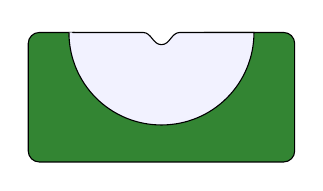
\begin{tikzpicture}[scale=.47]
        %Rand der Grafik
     \draw[rounded corners,cap=round,fill=green!40!black!80] (-3,-1)--(-3,-0)--(-1.5,0) -- (0,-1) -- (1.5,0) -- (4.2,0) -- (4.2,-3.5) -- (-3,-3.5) -- (-3,-1);
    % \draw[red] (-3,-2) circle (2pt){};

    % \draw[red] (-3,3) circle (2pt){};
    % \draw[red] (5,-2) circle (2pt){};
    % \draw[red] (5,3) circle (2pt){};
        \draw[cap=round,fill=blue!5] (-1.8,0) to  (0.1,0) to [out=0,in=180] (0.6,-0.33) to [out=0,in=180](1.1,0) to (3.1,0) [out=-90,in=0] to (0.6,-2.5) [out=180,in=-90] to (-1.9,0){};
            \draw  (-2.75,-0.12) node [right]{\textcolor{yellow!90!black!89!orange!90}{\rotatebox{0}{\scriptsize$\hrectangleblack$}}};
            \draw  (-2.71,-0.5) node [right]{\textcolor{yellow!90!black!89!orange!90}{\rotatebox{10}{\scriptsize$\hrectangleblack$}}};
            \draw  (-2.58,-0.94) node [right]{\textcolor{yellow!90!black!89!orange!90}{\rotatebox{20}{\scriptsize$\hrectangleblack$}}};
            \draw  (-2.38,-1.375) node [right]{\textcolor{yellow!90!black!89!orange!90}{\rotatebox{30}{\scriptsize$\hrectangleblack$}}};
            \draw  (-2.11,-1.76) node [right]{\textcolor{yellow!90!black!89!orange!90}{\rotatebox{40}{\scriptsize$\hrectangleblack$}}};
            \draw  (-1.76,-2.11) node [right]{\textcolor{yellow!90!black!89!orange!90}{\rotatebox{50}{\scriptsize$\hrectangleblack$}}};
            \draw  (-1.375,-2.38) node [right]{\textcolor{yellow!90!black!89!orange!90}{\rotatebox{60}{\scriptsize$\hrectangleblack$}}};
            \draw  (-0.94,-2.58) node [right]{\textcolor{yellow!90!black!89!orange!90}{\rotatebox{70}{\scriptsize$\hrectangleblack$}}};
            \draw  (-0.48,-2.71) node [right]{\textcolor{yellow!90!black!89!orange!90}{\rotatebox{80}{\scriptsize$\hrectangleblack$}}};
            \draw  (0.05,-2.75) node [right]{\textcolor{yellow!90!black!89!orange!90}{\rotatebox{90}{\scriptsize$\hrectangleblack$}}};
            \draw  (0.48,-2.71) node [right]{\textcolor{yellow!90!black!89!orange!90}{\rotatebox{100}{\scriptsize$\hrectangleblack$}}};
            \draw  (0.94,-2.58) node [right]{\textcolor{yellow!90!black!89!orange!90}{\rotatebox{110}{\scriptsize$\hrectangleblack$}}};
            \draw  (1.375,-2.38) node [right]{\textcolor{yellow!90!black!89!orange!90}{\rotatebox{120}{\scriptsize$\hrectangleblack$}}};
            \draw  (1.76,-2.11) node [right]{\textcolor{yellow!90!black!89!orange!90}{\rotatebox{130}{\scriptsize$\hrectangleblack$}}};
            \draw  (2.11,-1.76) node [right]{\textcolor{yellow!90!black!89!orange!90}{\rotatebox{140}{\scriptsize$\hrectangleblack$}}};
            \draw  (2.38,-1.375) node [right]{\textcolor{yellow!90!black!89!orange!90}{\rotatebox{150}{\scriptsize$\hrectangleblack$}}};
            \draw  (2.58,-0.94) node [right]{\textcolor{yellow!90!black!89!orange!90}{\rotatebox{160}{\scriptsize$\hrectangleblack$}}};
            \draw  (2.71,-0.5) node [right]{\textcolor{yellow!90!black!89!orange!90}{\rotatebox{170}{\scriptsize$\hrectangleblack$}}};
            \draw  (2.75,-0.12) node [right]{\textcolor{yellow!90!black!89!orange!90}{\rotatebox{180}{\scriptsize$\hrectangleblack$}}};
    \end{tikzpicture}\end{minipage}
    \begin{tikzpicture}[scale=1.2]
    %Rand der Grafik
    \draw[white] (-3,-1.5) circle (2pt){};
    \draw[white] (-3,2.5) circle (2pt){};
    \draw[white] (5,-1.5) circle (2pt){};
    \draw[white] (5,2.5) circle (2pt){};

%VELO stations
%below beam
    \draw[--,line width=1.5pt,green!40!black!80] (0.05,-0.25) --++ (0,.75){};
    \draw[--,line width=1.5pt,green!40!black!80] (0.25,-0.25) --++ (0,.75){};
    \draw[--,line width=1.5pt,green!40!black!80] (0.45,-0.25) --++ (0,.75){};
    \draw[--,line width=1.5pt,green!40!black!80] (0.65,-0.25) --++ (0,.75){};
    \draw[--,line width=1.5pt,green!40!black!80] (0.85,-0.25) --++ (0,.75){};
    \draw[--,line width=1.5pt,green!40!black!80] (1.05,-0.25) --++ (0,.75){};
     \draw[--,line width=1.5pt,green!40!black!80] (1.25,-0.25) --++ (0,.75){};
    \draw[--,line width=1.5pt,green!40!black!80] (1.45,-0.25) --++ (0,.75){};
    \draw[--,line width=1.5pt,green!40!black!80] (1.65,-0.25) --++ (0,.75){};
    \draw[--,line width=1.5pt,green!40!black!80] (1.85,-0.25) --++ (0,.75){};
    \draw[--,line width=1.5pt,green!40!black!80] (2.05,-0.25) --++ (0,.75){};
       
        \draw[--,line width=1.5pt,green!40!black!80] (2.55,-0.25) --++ (0,.75){};
        \draw[--,line width=1.5pt,green!40!black!80] (3.05,-0.25) --++ (0,.75){};
        \draw[--,line width=1.5pt,green!40!black!80] (3.55,-0.25) --++ (0,.75){};

        \draw[--,line width=1.5pt,green!40!black!80] (4.25,-0.25) --++ (0,.75){};
        \draw[--,line width=1.5pt,green!40!black!80] (4.45,-0.25) --++ (0,.75){};                
        \draw[--,line width=1.5pt,green!40!black!80] (4.65,-0.25) --++ (0,.75){};
        \draw[--,line width=1.5pt,green!40!black!80] (4.85,-0.25) --++ (0,.75){};
        
    \draw[--,line width=1.5pt,green!40!black!80] (-0.2,-0.25) --++ (0,.75){};
    \draw[--,line width=1.5pt,green!40!black!80] (-0.4,-0.25) --++ (0,.75){};
    \draw[--,line width=1.5pt,green!40!black!80] (-0.6,-0.25) --++ (0,.75){};
    \draw[--,line width=1.5pt,green!40!black!80] (-0.8,-0.25) --++ (0,.75){};
    \draw[--,line width=1.5pt,green!40!black!80] (-1.4,-0.25) --++ (0,.75){};
    \draw[--,line width=1.5pt,green!40!black!80] (-2,-0.25) --++ (0,.75){};
    \draw[--,line width=1.5pt,green!40!black!80] (-2.2,-0.25) --++ (0,.75){};
    \draw[--,line width=1.5pt,green!40!black!80] (-2.4,-0.25) --++ (0,.75){};
    \draw[--,line width=1.5pt,green!40!black!80] (-2.6,-0.25) --++ (0,.75){};
%above beam
    \draw[--,line width=1.5pt,green!40!black!80] (0,1) --++ (0,.75){};
    \draw[--,line width=1.5pt,green!40!black!80] (0.2,1) --++ (0,.75){};
    \draw[--,line width=1.5pt,green!40!black!80] (0.4,1) --++ (0,.75){};
    \draw[--,line width=1.5pt,green!40!black!80] (0.6,1) --++ (0,.75){};
    \draw[--,line width=1.5pt,green!40!black!80] (0.8,1) --++ (0,.75){};
    \draw[--,line width=1.5pt,green!40!black!80] (1,1) --++ (0,.75){};
     \draw[--,line width=1.5pt,green!40!black!80] (1.2,1) --++ (0,.75){};
    \draw[--,line width=1.5pt,green!40!black!80] (1.4,1) --++ (0,.75){};
    \draw[--,line width=1.5pt,green!40!black!80] (1.6,1) --++ (0,.75){};
    \draw[--,line width=1.5pt,green!40!black!80] (1.8,1) --++ (0,.75){};
    \draw[--,line width=1.5pt,green!40!black!80] (2,1) --++ (0,.75){};
       
        \draw[--,line width=1.5pt,green!40!black!80] (2.5,1) --++ (0,.75){};
        \draw[--,line width=1.5pt,green!40!black!80] (3,1) --++ (0,.75){};
        \draw[--,line width=1.5pt,green!40!black!80] (3.5,1) --++ (0,.75){};

        \draw[--,line width=1.5pt,green!40!black!80] (4.2,1) --++ (0,.75){};
        \draw[--,line width=1.5pt,green!40!black!80] (4.4,1) --++ (0,.75){};                
        \draw[--,line width=1.5pt,green!40!black!80] (4.6,1) --++ (0,.75){};
        \draw[--,line width=1.5pt,green!40!black!80] (4.8,1) --++ (0,.75){};
        
    \draw[--,line width=1.5pt,green!40!black!80] (-0.2,1) --++ (0,.75){};
    \draw[--,line width=1.5pt,green!40!black!80] (-0.4,1) --++ (0,.75){};
    \draw[--,line width=1.5pt,green!40!black!80] (-0.6,1) --++ (0,.75){};
    \draw[--,line width=1.5pt,green!40!black!80] (-0.8,1) --++ (0,.75){};
    \draw[--,line width=1.5pt,green!40!black!80] (-1.4,1) --++ (0,.75){};
    \draw[--,line width=1.5pt,green!40!black!80] (-2,1) --++ (0,.75){};
    \draw[--,line width=1.5pt,green!40!black!80] (-2.2,1) --++ (0,.75){};
    \draw[--,line width=1.5pt,green!40!black!80] (-2.4,1) --++ (0,.75){};
    \draw[--,line width=1.5pt,green!40!black!80] (-2.6,1) --++ (0,.75){};
%pp
\draw[->,line width=2pt](-0.5,.75) node [left] {$p$}--++ (0.5,0){};
\draw[->,line width=2pt](0.5,.75) node [right] {$p$}--++ (-0.5,0){};

%Labels 
\midlabelline{-3,-0.25}{-3,1.75}{\scriptsize\SI{6,6}{\centi\metre}}
\midlabelline{-2.6,-0.75}{4.9,-.75}{\scriptsize\SI{1}{\metre}}

%Events 
\node at (0.2,1) {\textcolor{red}{\scriptsize$\mathbf{\times}$}};
\node at (0.4,1.2) {\textcolor{red}{\scriptsize$\mathbf{\times}$}};
\node at (0.6,1.4) {\textcolor{red}{\scriptsize$\mathbf{\times}$}};
\node at (0.8,1.6) {\textcolor{red}{\scriptsize$\mathbf{\times}$}};


\node at (0.65,0.425) {\textcolor{red}{\scriptsize$\mathbf{\times}$}};
\node at (0.85,0.325) {\textcolor{red}{\scriptsize$\mathbf{\times}$}};
\node at (1.05,0.225) {\textcolor{red}{\scriptsize$\mathbf{\times}$}};

\node at (1.25,0.08) {\textcolor{red}{\scriptsize$\mathbf{\times}$}};
\node at (1.25,0.2) {\textcolor{red}{\scriptsize$\mathbf{\times}$}};

\node at (1.45,-0.08) {\textcolor{red}{\scriptsize$\mathbf{\times}$}};
\node at (1.45,0.2) {\textcolor{red}{\scriptsize$\mathbf{\times}$}};

\node at (1.65,-0.24) {\textcolor{red}{\scriptsize$\mathbf{\times}$}};
\node at (1.65,0.2) {\textcolor{red}{\scriptsize$\mathbf{\times}$}};

\node at (1.85,0.2) {\textcolor{red}{\scriptsize$\mathbf{\times}$}};
\node at (2.05,0.2) {\textcolor{red}{\scriptsize$\mathbf{\times}$}};
\node at (2.55,0.2) {\textcolor{red}{\scriptsize$\mathbf{\times}$}};
\node at (3.05,0.2) {\textcolor{red}{\scriptsize$\mathbf{\times}$}};
\node at (3.55,0.2) {\textcolor{red}{\scriptsize$\mathbf{\times}$}};
\node at (4.25,0.2) {\textcolor{red}{\scriptsize$\mathbf{\times}$}};
\node at (4.45,0.4) {\textcolor{red}{\scriptsize$\mathbf{\times}$}};
\node at (4.6,1.1) {\textcolor{red}{\scriptsize$\mathbf{\times}$}};
\node at (4.8,1.7) {\textcolor{red}{\scriptsize$\mathbf{\times}$}};

%Funktion

\draw[ rounded corners,cap=round,--,red!black!49,line width=2pt] (0,.8) -- (1.1,1.85){};
\draw[ rounded corners,cap=round,--,red,line width=2pt] (0,.75) -- (1.1,0.2){};
\draw[ rounded corners,cap=round,--,red,line width=2pt] (2,-0.52) -- (1.1,0.2){};
\draw[ rounded corners,cap=round,--,red,line width=2pt] (4.38,0.2) -- (1.1,0.2){};
\draw[ rounded corners,cap=round,--,red,line width=2pt] (4.38,0.2) -- (4.95,2.3){};
% \draw[ rounded corners,cap=round,--,red,line width=1pt,dashed] (4.38,0.2) -- (4.8,-0.3) node [right]{?};
    \end{tikzpicture}
\end{frame}
\begin{frame}{Vertex Locator (VELO)} \centering \addtocounter{framenumber}{-1}
\begin{minipage}{.59\textwidth}
    \begin{itemize}
        \item Spurrekonstruktion
        \item Identifikation von Vertices

    \end{itemize}
\end{minipage}
\begin{minipage}{.39\textwidth}
  \rotatebox{180}{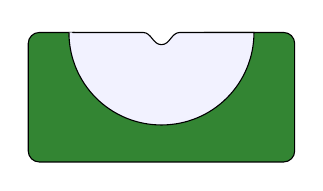
\begin{tikzpicture}[scale=.47]
        %Rand der Grafik
     \draw[rounded corners,cap=round,fill=green!40!black!80] (-3,-1)--(-3,-0)--(-1.5,0) -- (0,-1) -- (1.5,0) -- (4.2,0) -- (4.2,-3.5) -- (-3,-3.5) -- (-3,-1);
    % \draw[red] (-3,-2) circle (2pt){};

    % \draw[red] (-3,3) circle (2pt){};
    % \draw[red] (5,-2) circle (2pt){};
    % \draw[red] (5,3) circle (2pt){};
        \draw[cap=round,fill=blue!5] (-1.8,0) to  (0.1,0) to [out=0,in=180] (0.6,-0.33) to [out=0,in=180](1.1,0) to (3.1,0) [out=-90,in=0] to (0.6,-2.5) [out=180,in=-90] to (-1.9,0){};
            \draw  (-2.75,-0.12) node [right]{\textcolor{yellow!90!black!89!orange!90}{\rotatebox{0}{\scriptsize$\hrectangleblack$}}};
            \draw  (-2.71,-0.5) node [right]{\textcolor{yellow!90!black!89!orange!90}{\rotatebox{10}{\scriptsize$\hrectangleblack$}}};
            \draw  (-2.58,-0.94) node [right]{\textcolor{yellow!90!black!89!orange!90}{\rotatebox{20}{\scriptsize$\hrectangleblack$}}};
            \draw  (-2.38,-1.375) node [right]{\textcolor{yellow!90!black!89!orange!90}{\rotatebox{30}{\scriptsize$\hrectangleblack$}}};
            \draw  (-2.11,-1.76) node [right]{\textcolor{yellow!90!black!89!orange!90}{\rotatebox{40}{\scriptsize$\hrectangleblack$}}};
            \draw  (-1.76,-2.11) node [right]{\textcolor{yellow!90!black!89!orange!90}{\rotatebox{50}{\scriptsize$\hrectangleblack$}}};
            \draw  (-1.375,-2.38) node [right]{\textcolor{yellow!90!black!89!orange!90}{\rotatebox{60}{\scriptsize$\hrectangleblack$}}};
            \draw  (-0.94,-2.58) node [right]{\textcolor{yellow!90!black!89!orange!90}{\rotatebox{70}{\scriptsize$\hrectangleblack$}}};
            \draw  (-0.48,-2.71) node [right]{\textcolor{yellow!90!black!89!orange!90}{\rotatebox{80}{\scriptsize$\hrectangleblack$}}};
            \draw  (0.05,-2.75) node [right]{\textcolor{yellow!90!black!89!orange!90}{\rotatebox{90}{\scriptsize$\hrectangleblack$}}};
            \draw  (0.48,-2.71) node [right]{\textcolor{yellow!90!black!89!orange!90}{\rotatebox{100}{\scriptsize$\hrectangleblack$}}};
            \draw  (0.94,-2.58) node [right]{\textcolor{yellow!90!black!89!orange!90}{\rotatebox{110}{\scriptsize$\hrectangleblack$}}};
            \draw  (1.375,-2.38) node [right]{\textcolor{yellow!90!black!89!orange!90}{\rotatebox{120}{\scriptsize$\hrectangleblack$}}};
            \draw  (1.76,-2.11) node [right]{\textcolor{yellow!90!black!89!orange!90}{\rotatebox{130}{\scriptsize$\hrectangleblack$}}};
            \draw  (2.11,-1.76) node [right]{\textcolor{yellow!90!black!89!orange!90}{\rotatebox{140}{\scriptsize$\hrectangleblack$}}};
            \draw  (2.38,-1.375) node [right]{\textcolor{yellow!90!black!89!orange!90}{\rotatebox{150}{\scriptsize$\hrectangleblack$}}};
            \draw  (2.58,-0.94) node [right]{\textcolor{yellow!90!black!89!orange!90}{\rotatebox{160}{\scriptsize$\hrectangleblack$}}};
            \draw  (2.71,-0.5) node [right]{\textcolor{yellow!90!black!89!orange!90}{\rotatebox{170}{\scriptsize$\hrectangleblack$}}};
            \draw  (2.75,-0.12) node [right]{\textcolor{yellow!90!black!89!orange!90}{\rotatebox{180}{\scriptsize$\hrectangleblack$}}};
    \end{tikzpicture}} \\\vspace{-8pt}\\ 
    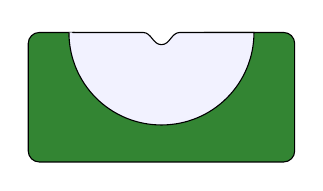
\begin{tikzpicture}[scale=.47]
        %Rand der Grafik
     \draw[rounded corners,cap=round,fill=green!40!black!80] (-3,-1)--(-3,-0)--(-1.5,0) -- (0,-1) -- (1.5,0) -- (4.2,0) -- (4.2,-3.5) -- (-3,-3.5) -- (-3,-1);
    % \draw[red] (-3,-2) circle (2pt){};

    % \draw[red] (-3,3) circle (2pt){};
    % \draw[red] (5,-2) circle (2pt){};
    % \draw[red] (5,3) circle (2pt){};
        \draw[cap=round,fill=blue!5] (-1.8,0) to  (0.1,0) to [out=0,in=180] (0.6,-0.33) to [out=0,in=180](1.1,0) to (3.1,0) [out=-90,in=0] to (0.6,-2.5) [out=180,in=-90] to (-1.9,0){};
            \draw  (-2.75,-0.12) node [right]{\textcolor{yellow!90!black!89!orange!90}{\rotatebox{0}{\scriptsize$\hrectangleblack$}}};
            \draw  (-2.71,-0.5) node [right]{\textcolor{yellow!90!black!89!orange!90}{\rotatebox{10}{\scriptsize$\hrectangleblack$}}};
            \draw  (-2.58,-0.94) node [right]{\textcolor{yellow!90!black!89!orange!90}{\rotatebox{20}{\scriptsize$\hrectangleblack$}}};
            \draw  (-2.38,-1.375) node [right]{\textcolor{yellow!90!black!89!orange!90}{\rotatebox{30}{\scriptsize$\hrectangleblack$}}};
            \draw  (-2.11,-1.76) node [right]{\textcolor{yellow!90!black!89!orange!90}{\rotatebox{40}{\scriptsize$\hrectangleblack$}}};
            \draw  (-1.76,-2.11) node [right]{\textcolor{yellow!90!black!89!orange!90}{\rotatebox{50}{\scriptsize$\hrectangleblack$}}};
            \draw  (-1.375,-2.38) node [right]{\textcolor{yellow!90!black!89!orange!90}{\rotatebox{60}{\scriptsize$\hrectangleblack$}}};
            \draw  (-0.94,-2.58) node [right]{\textcolor{yellow!90!black!89!orange!90}{\rotatebox{70}{\scriptsize$\hrectangleblack$}}};
            \draw  (-0.48,-2.71) node [right]{\textcolor{yellow!90!black!89!orange!90}{\rotatebox{80}{\scriptsize$\hrectangleblack$}}};
            \draw  (0.05,-2.75) node [right]{\textcolor{yellow!90!black!89!orange!90}{\rotatebox{90}{\scriptsize$\hrectangleblack$}}};
            \draw  (0.48,-2.71) node [right]{\textcolor{yellow!90!black!89!orange!90}{\rotatebox{100}{\scriptsize$\hrectangleblack$}}};
            \draw  (0.94,-2.58) node [right]{\textcolor{yellow!90!black!89!orange!90}{\rotatebox{110}{\scriptsize$\hrectangleblack$}}};
            \draw  (1.375,-2.38) node [right]{\textcolor{yellow!90!black!89!orange!90}{\rotatebox{120}{\scriptsize$\hrectangleblack$}}};
            \draw  (1.76,-2.11) node [right]{\textcolor{yellow!90!black!89!orange!90}{\rotatebox{130}{\scriptsize$\hrectangleblack$}}};
            \draw  (2.11,-1.76) node [right]{\textcolor{yellow!90!black!89!orange!90}{\rotatebox{140}{\scriptsize$\hrectangleblack$}}};
            \draw  (2.38,-1.375) node [right]{\textcolor{yellow!90!black!89!orange!90}{\rotatebox{150}{\scriptsize$\hrectangleblack$}}};
            \draw  (2.58,-0.94) node [right]{\textcolor{yellow!90!black!89!orange!90}{\rotatebox{160}{\scriptsize$\hrectangleblack$}}};
            \draw  (2.71,-0.5) node [right]{\textcolor{yellow!90!black!89!orange!90}{\rotatebox{170}{\scriptsize$\hrectangleblack$}}};
            \draw  (2.75,-0.12) node [right]{\textcolor{yellow!90!black!89!orange!90}{\rotatebox{180}{\scriptsize$\hrectangleblack$}}};
    \end{tikzpicture}\end{minipage}
    \begin{tikzpicture}[scale=1.2]
    %Rand der Grafik
    \draw[white] (-3,-1.5) circle (2pt){};
    \draw[white] (-3,2.5) circle (2pt){};
    \draw[white] (5,-1.5) circle (2pt){};
    \draw[white] (5,2.5) circle (2pt){};

%VELO stations
%below beam
    \draw[--,line width=1.5pt,green!40!black!80] (0.05,-0.25) --++ (0,.75){};
    \draw[--,line width=1.5pt,green!40!black!80] (0.25,-0.25) --++ (0,.75){};
    \draw[--,line width=1.5pt,green!40!black!80] (0.45,-0.25) --++ (0,.75){};
    \draw[--,line width=1.5pt,green!40!black!80] (0.65,-0.25) --++ (0,.75){};
    \draw[--,line width=1.5pt,green!40!black!80] (0.85,-0.25) --++ (0,.75){};
    \draw[--,line width=1.5pt,green!40!black!80] (1.05,-0.25) --++ (0,.75){};
     \draw[--,line width=1.5pt,green!40!black!80] (1.25,-0.25) --++ (0,.75){};
    \draw[--,line width=1.5pt,green!40!black!80] (1.45,-0.25) --++ (0,.75){};
    \draw[--,line width=1.5pt,green!40!black!80] (1.65,-0.25) --++ (0,.75){};
    \draw[--,line width=1.5pt,green!40!black!80] (1.85,-0.25) --++ (0,.75){};
    \draw[--,line width=1.5pt,green!40!black!80] (2.05,-0.25) --++ (0,.75){};
       
        \draw[--,line width=1.5pt,green!40!black!80] (2.55,-0.25) --++ (0,.75){};
        \draw[--,line width=1.5pt,green!40!black!80] (3.05,-0.25) --++ (0,.75){};
        \draw[--,line width=1.5pt,green!40!black!80] (3.55,-0.25) --++ (0,.75){};

        \draw[--,line width=1.5pt,green!40!black!80] (4.25,-0.25) --++ (0,.75){};
        \draw[--,line width=1.5pt,green!40!black!80] (4.45,-0.25) --++ (0,.75){};                
        \draw[--,line width=1.5pt,green!40!black!80] (4.65,-0.25) --++ (0,.75){};
        \draw[--,line width=1.5pt,green!40!black!80] (4.85,-0.25) --++ (0,.75){};
        
    \draw[--,line width=1.5pt,green!40!black!80] (-0.2,-0.25) --++ (0,.75){};
    \draw[--,line width=1.5pt,green!40!black!80] (-0.4,-0.25) --++ (0,.75){};
    \draw[--,line width=1.5pt,green!40!black!80] (-0.6,-0.25) --++ (0,.75){};
    \draw[--,line width=1.5pt,green!40!black!80] (-0.8,-0.25) --++ (0,.75){};
    \draw[--,line width=1.5pt,green!40!black!80] (-1.4,-0.25) --++ (0,.75){};
    \draw[--,line width=1.5pt,green!40!black!80] (-2,-0.25) --++ (0,.75){};
    \draw[--,line width=1.5pt,green!40!black!80] (-2.2,-0.25) --++ (0,.75){};
    \draw[--,line width=1.5pt,green!40!black!80] (-2.4,-0.25) --++ (0,.75){};
    \draw[--,line width=1.5pt,green!40!black!80] (-2.6,-0.25) --++ (0,.75){};
%above beam
    \draw[--,line width=1.5pt,green!40!black!80] (0,1) --++ (0,.75){};
    \draw[--,line width=1.5pt,green!40!black!80] (0.2,1) --++ (0,.75){};
    \draw[--,line width=1.5pt,green!40!black!80] (0.4,1) --++ (0,.75){};
    \draw[--,line width=1.5pt,green!40!black!80] (0.6,1) --++ (0,.75){};
    \draw[--,line width=1.5pt,green!40!black!80] (0.8,1) --++ (0,.75){};
    \draw[--,line width=1.5pt,green!40!black!80] (1,1) --++ (0,.75){};
     \draw[--,line width=1.5pt,green!40!black!80] (1.2,1) --++ (0,.75){};
    \draw[--,line width=1.5pt,green!40!black!80] (1.4,1) --++ (0,.75){};
    \draw[--,line width=1.5pt,green!40!black!80] (1.6,1) --++ (0,.75){};
    \draw[--,line width=1.5pt,green!40!black!80] (1.8,1) --++ (0,.75){};
    \draw[--,line width=1.5pt,green!40!black!80] (2,1) --++ (0,.75){};
       
        \draw[--,line width=1.5pt,green!40!black!80] (2.5,1) --++ (0,.75){};
        \draw[--,line width=1.5pt,green!40!black!80] (3,1) --++ (0,.75){};
        \draw[--,line width=1.5pt,green!40!black!80] (3.5,1) --++ (0,.75){};

        \draw[--,line width=1.5pt,green!40!black!80] (4.2,1) --++ (0,.75){};
        \draw[--,line width=1.5pt,green!40!black!80] (4.4,1) --++ (0,.75){};                
        \draw[--,line width=1.5pt,green!40!black!80] (4.6,1) --++ (0,.75){};
        \draw[--,line width=1.5pt,green!40!black!80] (4.8,1) --++ (0,.75){};
        
    \draw[--,line width=1.5pt,green!40!black!80] (-0.2,1) --++ (0,.75){};
    \draw[--,line width=1.5pt,green!40!black!80] (-0.4,1) --++ (0,.75){};
    \draw[--,line width=1.5pt,green!40!black!80] (-0.6,1) --++ (0,.75){};
    \draw[--,line width=1.5pt,green!40!black!80] (-0.8,1) --++ (0,.75){};
    \draw[--,line width=1.5pt,green!40!black!80] (-1.4,1) --++ (0,.75){};
    \draw[--,line width=1.5pt,green!40!black!80] (-2,1) --++ (0,.75){};
    \draw[--,line width=1.5pt,green!40!black!80] (-2.2,1) --++ (0,.75){};
    \draw[--,line width=1.5pt,green!40!black!80] (-2.4,1) --++ (0,.75){};
    \draw[--,line width=1.5pt,green!40!black!80] (-2.6,1) --++ (0,.75){};
%pp
\draw[->,line width=2pt](-0.5,.75) node [left] {$p$}--++ (0.5,0){};
\draw[->,line width=2pt](0.5,.75) node [right] {$p$}--++ (-0.5,0){};

%Labels 
\midlabelline{-3,-0.25}{-3,1.75}{\scriptsize\SI{6,6}{\centi\metre}}
\midlabelline{-2.6,-0.75}{4.9,-.75}{\scriptsize\SI{1}{\metre}}

%Events 
\node at (0.2,1) {\textcolor{red}{\scriptsize$\mathbf{\times}$}};
\node at (0.4,1.2) {\textcolor{red}{\scriptsize$\mathbf{\times}$}};
\node at (0.6,1.4) {\textcolor{red}{\scriptsize$\mathbf{\times}$}};
\node at (0.8,1.6) {\textcolor{red}{\scriptsize$\mathbf{\times}$}};


\node at (0.65,0.425) {\textcolor{red}{\scriptsize$\mathbf{\times}$}};
\node at (0.85,0.325) {\textcolor{red}{\scriptsize$\mathbf{\times}$}};
\node at (1.05,0.225) {\textcolor{red}{\scriptsize$\mathbf{\times}$}};

\node at (1.25,0.08) {\textcolor{red}{\scriptsize$\mathbf{\times}$}};
\node at (1.25,0.2) {\textcolor{red}{\scriptsize$\mathbf{\times}$}};

\node at (1.45,-0.08) {\textcolor{red}{\scriptsize$\mathbf{\times}$}};
\node at (1.45,0.2) {\textcolor{red}{\scriptsize$\mathbf{\times}$}};

\node at (1.65,-0.24) {\textcolor{red}{\scriptsize$\mathbf{\times}$}};
\node at (1.65,0.2) {\textcolor{red}{\scriptsize$\mathbf{\times}$}};

\node at (1.85,0.2) {\textcolor{red}{\scriptsize$\mathbf{\times}$}};
\node at (2.05,0.2) {\textcolor{red}{\scriptsize$\mathbf{\times}$}};
\node at (2.55,0.2) {\textcolor{red}{\scriptsize$\mathbf{\times}$}};
\node at (3.05,0.2) {\textcolor{red}{\scriptsize$\mathbf{\times}$}};
\node at (3.55,0.2) {\textcolor{red}{\scriptsize$\mathbf{\times}$}};
\node at (4.25,0.2) {\textcolor{red}{\scriptsize$\mathbf{\times}$}};
\node at (4.45,0.4) {\textcolor{red}{\scriptsize$\mathbf{\times}$}};
\node at (4.6,1.1) {\textcolor{red}{\scriptsize$\mathbf{\times}$}};
\node at (4.8,1.7) {\textcolor{red}{\scriptsize$\mathbf{\times}$}};

%Funktion

\draw[ rounded corners,cap=round,--,red!black!49,line width=2pt] (0,.8) -- (1.1,1.85){};
\draw[ rounded corners,cap=round,--,red,line width=2pt] (0,.75) -- (1.1,0.2){};
\draw[ rounded corners,cap=round,--,red,line width=2pt] (2,-0.52) -- (1.1,0.2){};
\draw[ rounded corners,cap=round,--,red,line width=2pt] (4.38,0.2) -- (1.1,0.2){};
\draw[ rounded corners,cap=round,--,red,line width=2pt] (4.38,0.2) -- (4.95,2.3){};
\draw[ rounded corners,cap=round,--,red,line width=1pt,dashed] (4.38,0.2) -- (4.8,-0.3) node [right]{?};
    \end{tikzpicture}
\end{frame}
%%%%%%%%%%%%%%%%%%%%%%%%%%%%%%%%%%%%%%%%%%%%%%%%%%%%%%%%%%%%%%%%%%%%%%%%%%%%%%%%%%%%%%%%%%%%%%
\begin{frame}{Ring Imaging Cherenkov Detector (RICH1)}
    \begin{minipage}{0.68\textwidth}
    \begin{itemize}
        \item Misst \textcolor{red}{\textbf{Geschwindigkeit}} der Teilchen
        \item Wichtig für Identifikation von Teilchen
        \item Nur in begrenztem Impulsfenster definiert
    \end{itemize}
    \end{minipage}\hfill
    \begin{minipage}{0.28\textwidth}
        \begin{figure}[h]
        \centering
        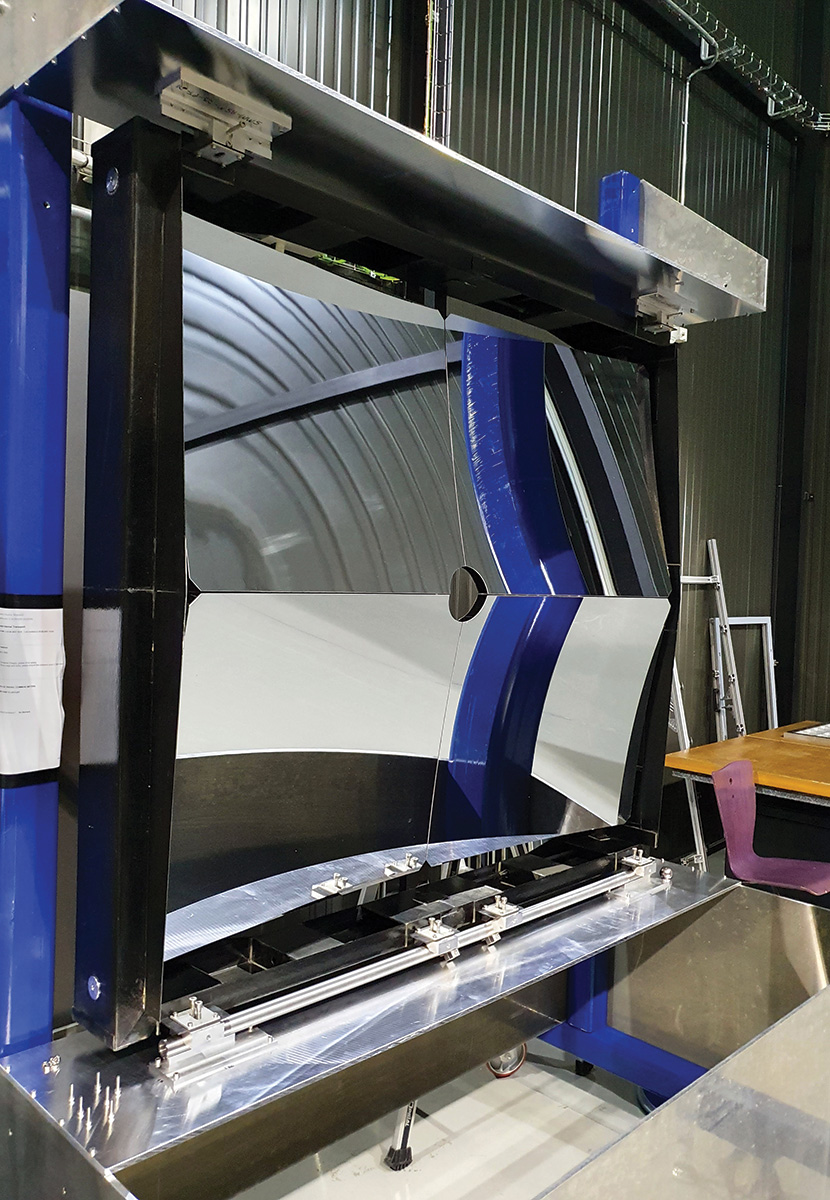
\includegraphics[height=3cm]{Figures Introductory Lecture/LHCb Detector/LHCb_RICH1.jpeg}%source:https://cds.cern.ch/record/2807064
        \end{figure}
    \end{minipage}
    \vspace{-0.5cm}
    \begin{figure}[h]
    \centering
    \begin{overpic}[width=0.8\textwidth]{Figures Introductory Lecture/LHCb Detector/LHCb_2.png}
      
        \put (13,45) {\colorbox{LHCbDarkBlue!80}{\textcolor{LHCbLightBlue}{\centering \tiny  RICH 1}}}
        \put (3,35) {\colorbox{lightgray}{\centering \tiny  VELO}}

\put (1,5) {\tiny $z/m \rightarrow$}
\put (17.5,2) {\tiny $2$}
    
    \end{overpic}
    \end{figure}
\end{frame}
\begin{frame}
    \begin{figure}[h]
        \centering
        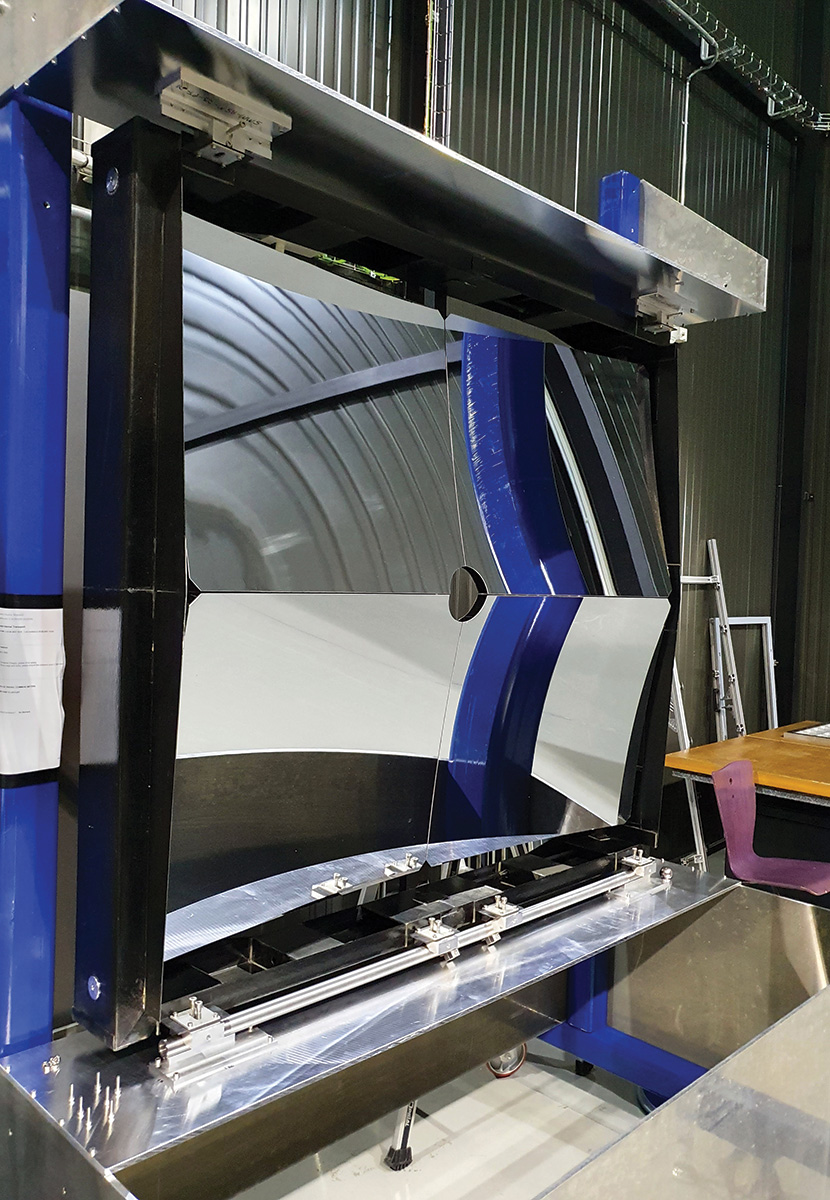
\includegraphics[height=\textheight]{Figures Introductory Lecture/LHCb Detector/LHCb_RICH1.jpeg}%source:https://cds.cern.ch/record/2807064
        \end{figure}
\end{frame}
\begin{frame}{Cherenkov Effekt}
    \begin{minipage}{.49\textwidth}
     \begin{tikzpicture}
\draw[--,fill=red!20!orange!30](-3,-2)--(0,-2)--(0,2)--(-3,2)--(-3,-2){};
         \draw[--,blue] (-2,-0.5)--(-2.5,0)--(-2,0.5){};
         \draw[--,blue] (-1.5,-0.5)--(-2,0)--(-1.5,0.5){};
         \draw[--,blue] (-1,-0.5)--(-1.5,0)--(-1,0.5){};
                  
        \node at (-2,-1) {$n>n_0$};
        \node at (-4,-1) {$n_0$};
        \node at (-1.5,2.5) {RICH};        \node at (-1.5,-2.5) {~};
        \node at (-2,-1.5) {$c=\frac{c_{\text{vak.}}}{n}$};
        \node at (-4,-1.5) {$c=\frac{c_{\text{vak.}}}{n_0}$};
         \draw[->,line width=2pt](-5,0) to node [above] {$v$}(-3,0) to (0.5,0){};
     \end{tikzpicture}   
    \end{minipage}
        \begin{minipage}{.49\textwidth}
        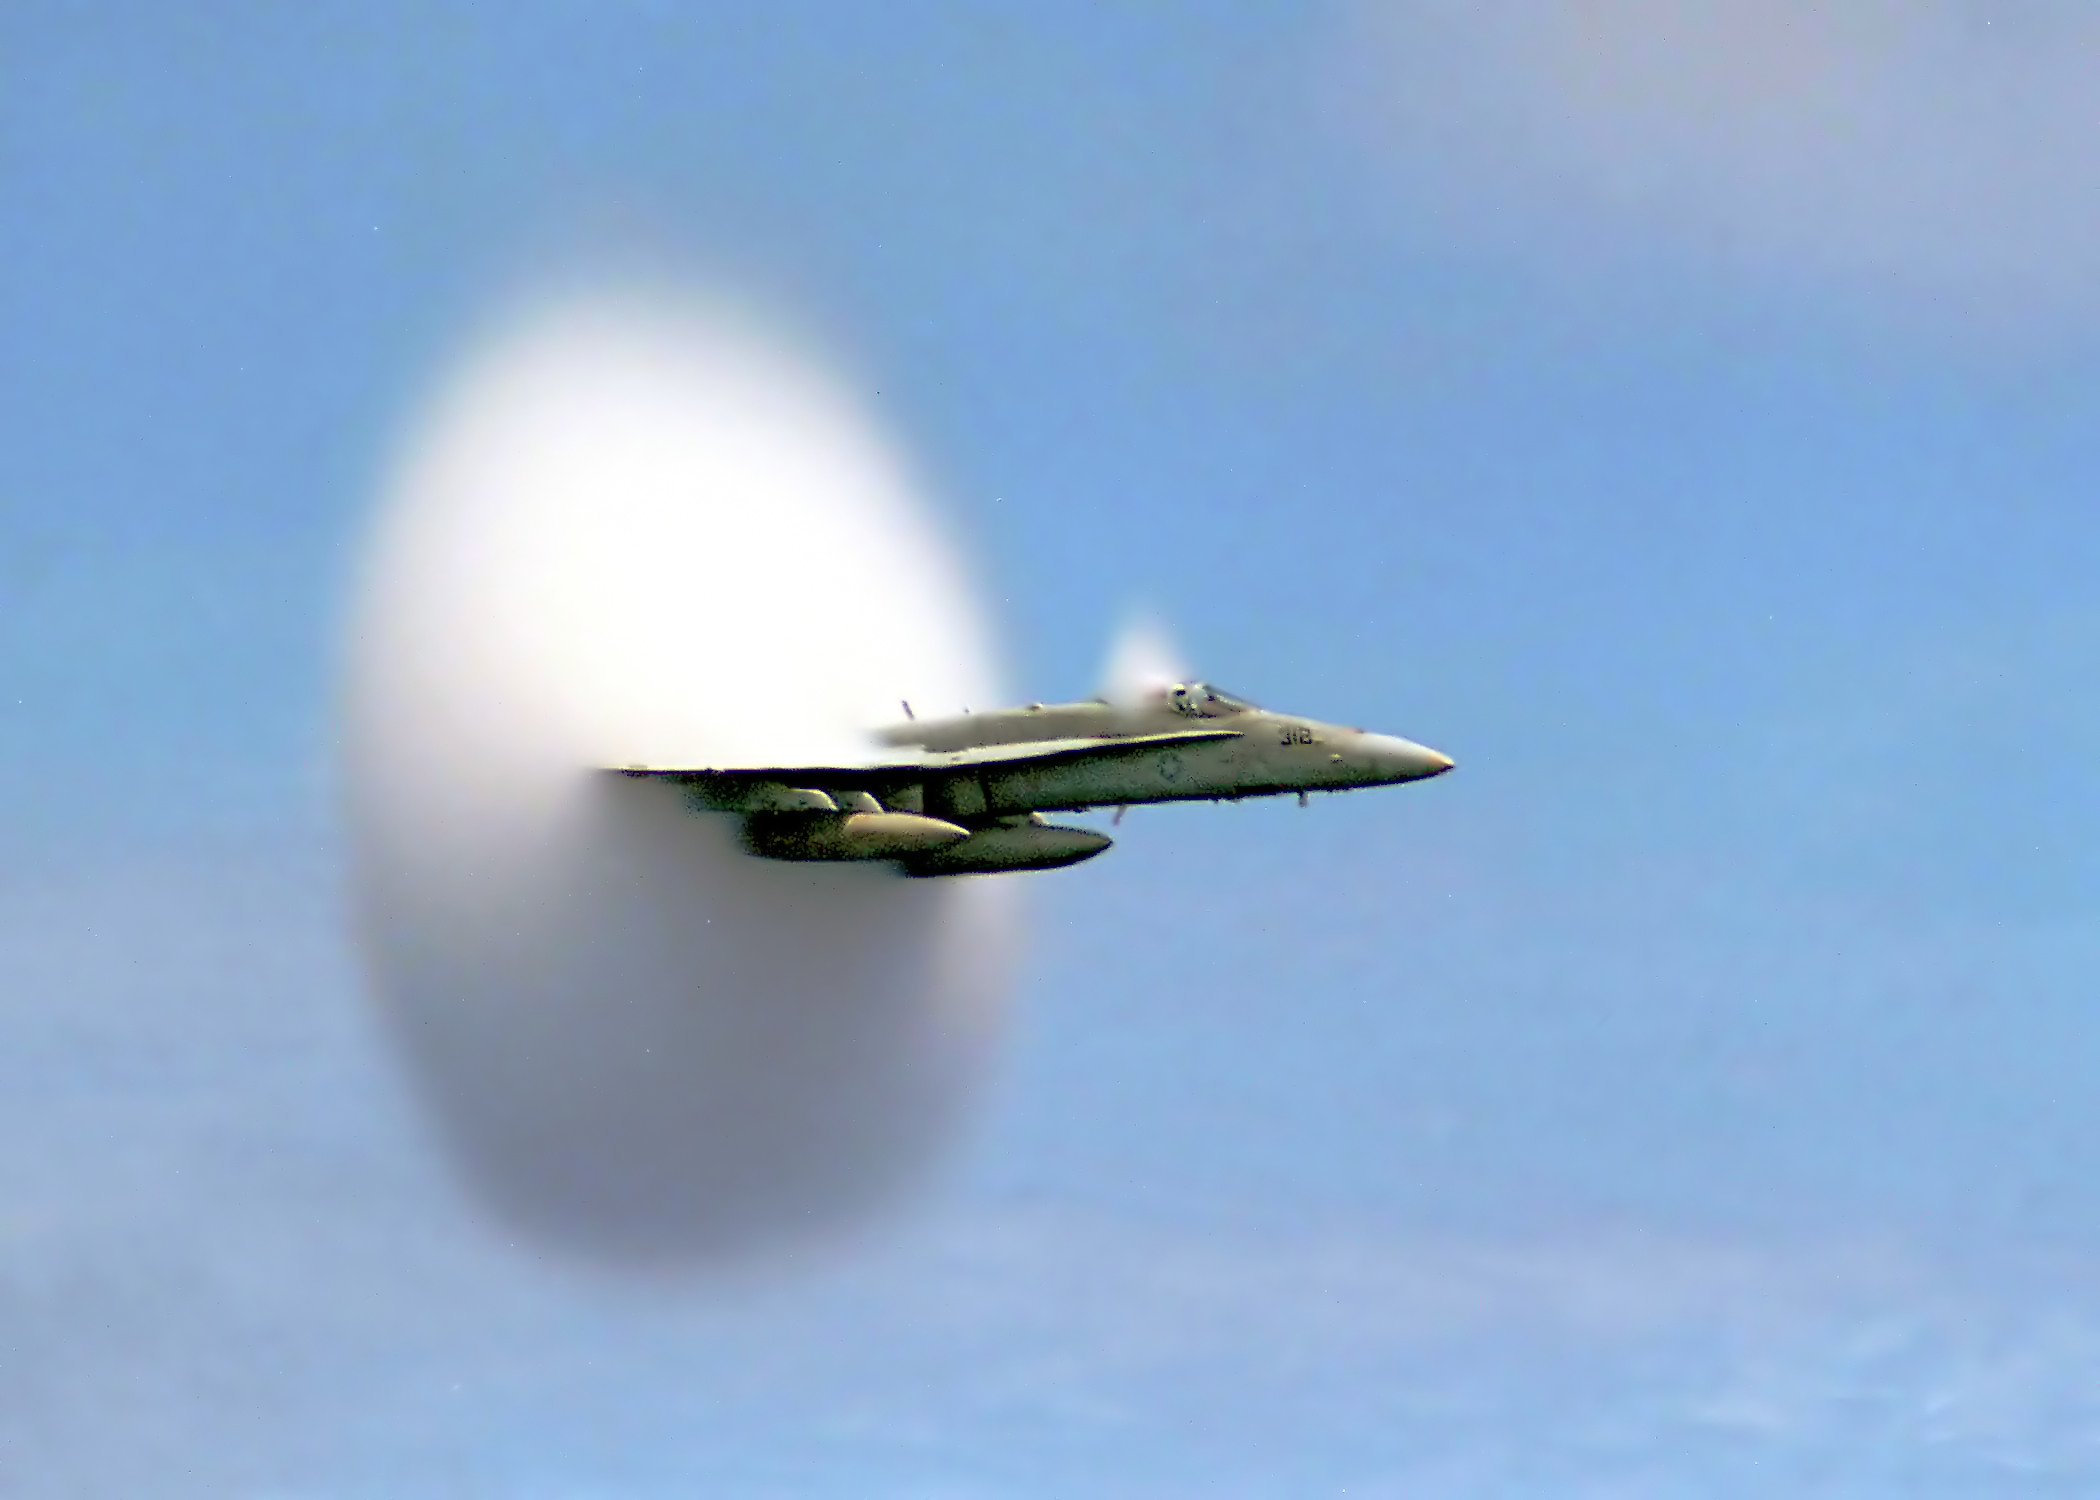
\includegraphics[width=\textwidth]{Figures Introductory Lecture/FA-18-Jet.jpg}
    \end{minipage}
    \vspace{1cm}
    Für $v>c$ wird Strahlung emittiert! Die kann man messen.

    
    
\end{frame}
\begin{frame}{Cherenkov Effekt in Wasser $n\approx1.3$}
    \begin{minipage}{.49\textwidth}
    \begin{tikzpicture}[scale=0.8] \draw[black,fill=blue!20,line width=2pt] (-1.5,0.5) circle (2.35cm){};
        \draw[--,line width=2pt] (0,0)--(-1.5,1.5)--(-3,0){};
        \node[circle,shading=ball,ball color=red] (ball) at (0,0) {\textbf{\sffamily \HUGE \textcolor{white}{H}}};
        \node[circle,shading=ball,ball color=red] (ball) at (-3,0) {\textbf{\sffamily \HUGE \textcolor{white}{H}}};
        \node[circle,shading=ball,ball color=blue] (ball) at (-1.5,1.5) {\textbf{\sffamily \HUGE \textcolor{white}{O}}};
       % \draw [->,green!50!black!77,line width=4pt] (-1.5,1.3)--(-1.5,-.7) node [below,black] {$p$};
        \node at (-0.9,2) {$\delta^-$};
        \node at (-3.5,0.5) {$\delta^+$};
        \node at (0.6,0.5) {$\delta^+$};
         \node at (1,-4) {~};
    \end{tikzpicture}
    \end{minipage}
    \begin{minipage}{.49\textwidth}
    \begin{tikzpicture}\boldmath 
        %\draw[->,line width=1pt] (0,3)--(0,-3);
         % \shade[ball color=green] (0,0) circle (8pt) node [black]{\textbf{\sffamily $e^-$}};
          \draw[--,round corners=2pt,line width=2pt,fill=blue!10] (-3,0)--(-3,-2)--(3,-2)--(3,2)--(-3,2)-- (-3,0){};
\def\x{-2.5}
        \node (A05) at (\x,1.25); \def\R{90} \draw[black, fill=blue!20,rotate=\R] (A05) circle  (6pt);

        \node (B05) at (\x,0.75); \def\R{90} \draw[black, fill=blue!20,rotate=\R] (B05) circle  (6pt);

        \node (C05) at (\x,0.25); \def\R{90} \draw[black, fill=blue!20,rotate=\R] (C05) circle  (6pt);

        \node (D05) at (\x,-0.25); \def\R{90} \draw[black, fill=blue!20,rotate=\R] (D05) circle  (6pt);

        \node (E05) at (\x,-0.75); \def\R{90} \draw[black, fill=blue!20,rotate=\R] (E05) circle  (6pt);

        \node (F05) at (\x,-1.25); \def\R{90} \draw[black, fill=blue!20,rotate=\R] (F05) circle  (6pt);

\def\x{-1.5}
        \node (A05) at (\x,1.25); \def\R{90} \draw[black, fill=blue!20,rotate=\R] (A05) circle  (6pt);

        \node (B05) at (\x,0.75); \def\R{90} \draw[black, fill=blue!20,rotate=\R] (B05) circle  (6pt);

        \node (C05) at (\x,0.25); \def\R{90} \draw[black, fill=blue!20,rotate=\R] (C05) circle  (6pt);

        \node (D05) at (\x,-0.25); \def\R{90} \draw[black, fill=blue!20,rotate=\R] (D05) circle  (6pt);

        \node (E05) at (\x,-0.75); \def\R{90} \draw[black, fill=blue!20,rotate=\R] (E05) circle  (6pt);

        \node (F05) at (\x,-1.25); \def\R{90} \draw[black, fill=blue!20,rotate=\R] (F05) circle  (6pt);

\def\x{-0.5}
        \node (A05) at (\x,1.25); \def\R{90} \draw[black, fill=blue!20,rotate=\R] (A05) circle  (6pt);

        \node (B05) at (\x,0.75); \def\R{90} \draw[black, fill=blue!20,rotate=\R] (B05) circle  (6pt);

        \node (C05) at (\x,0.25); \def\R{90} \draw[black, fill=blue!20,rotate=\R] (C05) circle  (6pt);

        \node (D05) at (\x,-0.25); \def\R{90} \draw[black, fill=blue!20,rotate=\R] (D05) circle  (6pt);

        \node (E05) at (\x,-0.75); \def\R{90} \draw[black, fill=blue!20,rotate=\R] (E05) circle  (6pt);

        \node (F05) at (\x,-1.25); \def\R{90} \draw[black, fill=blue!20,rotate=\R] (F05) circle  (6pt);

\def\x{0.5}
        \node (A05) at (\x,1.25); \def\R{90} \draw[black, fill=blue!20,rotate=\R] (A05) circle  (6pt);

        \node (B05) at (\x,0.75); \def\R{90} \draw[black, fill=blue!20,rotate=\R] (B05) circle  (6pt);

        \node (C05) at (\x,0.25); \def\R{90} \draw[black, fill=blue!20,rotate=\R] (C05) circle  (6pt);

        \node (D05) at (\x,-0.25); \def\R{90} \draw[black, fill=blue!20,rotate=\R] (D05) circle  (6pt);

        \node (E05) at (\x,-0.75); \def\R{90} \draw[black, fill=blue!20,rotate=\R] (E05) circle  (6pt);

        \node (F05) at (\x,-1.25); \def\R{90} \draw[black, fill=blue!20,rotate=\R] (F05) circle  (6pt);

\def\x{1.5}
        \node (A05) at (\x,1.25); \def\R{90} \draw[black, fill=blue!20,rotate=\R] (A05) circle  (6pt);

        \node (B05) at (\x,0.75); \def\R{90} \draw[black, fill=blue!20,rotate=\R] (B05) circle  (6pt);

        \node (C05) at (\x,0.25); \def\R{90} \draw[black, fill=blue!20,rotate=\R] (C05) circle  (6pt);

        \node (D05) at (\x,-0.25); \def\R{90} \draw[black, fill=blue!20,rotate=\R] (D05) circle  (6pt);

        \node (E05) at (\x,-0.75); \def\R{90} \draw[black, fill=blue!20,rotate=\R] (E05) circle  (6pt);

        \node (F05) at (\x,-1.25); \def\R{90} \draw[black, fill=blue!20,rotate=\R] (F05) circle  (6pt);

\def\x{2.5}
        \node (A05) at (\x,1.25); \def\R{90} \draw[black, fill=blue!20,rotate=\R] (A05) circle  (6pt);

        \node (B05) at (\x,0.75); \def\R{90} \draw[black, fill=blue!20,rotate=\R] (B05) circle  (6pt);

        \node (C05) at (\x,0.25); \def\R{90} \draw[black, fill=blue!20,rotate=\R] (C05) circle  (6pt);

        \node (D05) at (\x,-0.25); \def\R{90} \draw[black, fill=blue!20,rotate=\R] (D05) circle  (6pt);

        \node (E05) at (\x,-0.75); \def\R{90} \draw[black, fill=blue!20,rotate=\R] (E05) circle  (6pt);

        \node (F05) at (\x,-1.25); \def\R{90} \draw[black, fill=blue!20,rotate=\R] (F05) circle  (6pt);

\def\x{1}
        \node (A1) at (\x,1); \def\R{90} \draw[black, fill=blue!20,rotate=\R] (A1) circle  (6pt);

        \node (B1) at (\x,0.5); \def\R{90} \draw[black, fill=blue!20,rotate=\R] (B1) circle  (6pt);

        \node (C1) at (\x,0); \def\R{90} \draw[black, fill=blue!20,rotate=\R] (C1) circle  (6pt);

        \node (D1) at (\x,-0.5); \def\R{90} \draw[black, fill=blue!20,rotate=\R] (D1) circle  (6pt);

        \node (E1) at (\x,-1); \def\R{90} \draw[black, fill=blue!20,rotate=\R] (E1) circle  (6pt);

         \node (F1) at (\x,-1.5); \def\R{90} \draw[black, fill=blue!20,rotate=\R] (F1) circle  (6pt);

         \node (G1) at (\x,1.5); \def\R{90} \draw[black, fill=blue!20,rotate=\R] (G1) circle  (6pt);
\def\x{2}
        \node (A1) at (\x,1); \def\R{90} \draw[black, fill=blue!20,rotate=\R] (A1) circle  (6pt);

        \node (B1) at (\x,0.5); \def\R{90} \draw[black, fill=blue!20,rotate=\R] (B1) circle  (6pt);

        \node (C1) at (\x,0); \def\R{90} \draw[black, fill=blue!20,rotate=\R] (C1) circle  (6pt);

        \node (D1) at (\x,-0.5); \def\R{90} \draw[black, fill=blue!20,rotate=\R] (D1) circle  (6pt);

        \node (E1) at (\x,-1); \def\R{90} \draw[black, fill=blue!20,rotate=\R] (E1) circle  (6pt);

         \node (F1) at (\x,-1.5); \def\R{90} \draw[black, fill=blue!20,rotate=\R] (F1) circle  (6pt);

         \node (G1) at (\x,1.5); \def\R{90} \draw[black, fill=blue!20,rotate=\R] (G1) circle  (6pt);
\def\x{-1}
        \node (A1) at (\x,1); \def\R{90} \draw[black, fill=blue!20,rotate=\R] (A1) circle  (6pt);

        \node (B1) at (\x,0.5); \def\R{90} \draw[black, fill=blue!20,rotate=\R] (B1) circle  (6pt);

        \node (C1) at (\x,0); \def\R{90} \draw[black, fill=blue!20,rotate=\R] (C1) circle  (6pt);

        \node (D1) at (\x,-0.5); \def\R{90} \draw[black, fill=blue!20,rotate=\R] (D1) circle  (6pt);

        \node (E1) at (\x,-1); \def\R{90} \draw[black, fill=blue!20,rotate=\R] (E1) circle  (6pt);

         \node (F1) at (\x,-1.5); \def\R{90} \draw[black, fill=blue!20,rotate=\R] (F1) circle  (6pt);

         \node (G1) at (\x,1.5); \def\R{90} \draw[black, fill=blue!20,rotate=\R] (G1) circle  (6pt);
\def\x{-2}
        \node (A1) at (\x,1); \def\R{90} \draw[black, fill=blue!20,rotate=\R] (A1) circle  (6pt);

        \node (B1) at (\x,0.5); \def\R{90} \draw[black, fill=blue!20,rotate=\R] (B1) circle  (6pt);

        \node (C1) at (\x,0); \def\R{90} \draw[black, fill=blue!20,rotate=\R] (C1) circle  (6pt);

        \node (D1) at (\x,-0.5); \def\R{90} \draw[black, fill=blue!20,rotate=\R] (D1) circle  (6pt);

        \node (E1) at (\x,-1); \def\R{90} \draw[black, fill=blue!20,rotate=\R] (E1) circle  (6pt);

         \node (F1) at (\x,-1.5); \def\R{90} \draw[black, fill=blue!20,rotate=\R] (F1) circle  (6pt);

         \node (G1) at (\x,1.5); \def\R{90} \draw[black, fill=blue!20,rotate=\R] (G1) circle  (6pt);
        


    \end{tikzpicture}
           
    
    \end{minipage}
\[ ~\]
\end{frame}
\begin{frame}{Cherenkov Effekt in Wasser $n\approx1.3$}
    \begin{minipage}{.49\textwidth}
    \begin{tikzpicture}\boldmath 
        \clip (-2,-3.2) rectangle (2,3); % Ausschnitt definieren
        \draw[->,line width=1pt] (0,3)--(0,-3) node [right] {$v$};
        \draw[--,line width=1pt](-2,0.5)--(0,-0.5)--(2,0.5){};
        \draw[--,dashed,black!100] (0,0) circle (12.5pt){};
        \draw[--,dashed,black!100] (0,0.5) circle (25pt){};
        \draw[--,dashed,black!80] (0,1) circle (37.5pt){};
        \draw[--,dashed,black!60] (0,1.5) circle (50pt){};
        \draw[--,dashed,black!40] (0,2) circle (62.5pt){};
        \draw[--,dashed,black!20] (0,3) circle (87.5pt){};
        \shade[ball color=green] (0,-0.5) circle (8pt) node [black]{\textbf{\sffamily $e^-$}};
        \draw[->,blue,line width=2pt](1,0)--(1.5,-1) node [below] {$\gamma$};
        \draw[--,blue,line width=1pt,dashed](0,2)--(1,0);
        \draw[->,blue,line width=2pt](-1,0)--(-1.5,-1) node [below] {$\gamma$};
        \draw[--,blue,line width=1pt,dashed](0,2)--(-1,0);
        \draw[--,black,line width=1pt](0,0.75) [out=-360,in=-165]  to node [below] {$\theta$} (0.6,0.85){};
    \end{tikzpicture}
    \end{minipage}
    \begin{minipage}{.49\textwidth}
    \begin{tikzpicture}\boldmath 
         \draw[--,round corners=2pt,line width=2pt,fill=blue!10] (-3,0)--(-3,-2)--(3,-2)--(3,2)--(-3,2)-- (-3,0){};
        \draw[->,line width=1pt] (0,3)--(0,-3)node [right] {$v$};
          \shade[ball color=green] (0,-0.5) circle (8pt) node [black]{\textbf{\sffamily $e^-$}};


\def\x{-2.5}
        \node (A05) at (\x,1.25); \def\R{90} \draw[black, fill=blue!20,rotate=\R] (A05) circle  (6pt);

        \node (B05) at (\x,0.75); \def\R{90} \draw[black, fill=blue!20,rotate=\R] (B05) circle  (6pt);

        \node (C05) at (\x,0.25); \def\R{90} \draw[black, fill=blue!20,rotate=\R] (C05) circle  (6pt);

        \node (D05) at (\x,-0.25); \def\R{90} \draw[black, fill=blue!20,rotate=\R] (D05) circle  (6pt);

        \node (E05) at (\x,-0.75); \def\R{90} \draw[black, fill=blue!20,rotate=\R] (E05) circle  (6pt);

        \node (F05) at (\x,-1.25); \def\R{90} \draw[black, fill=blue!20,rotate=\R] (F05) circle  (6pt);
        
\def\x{-2}
        \node (A1) at (\x,1); \def\R{-110} \draw[black, fill=blue!20,rotate=\R] (A1) ellipse  (5.9pt and 6.1pt) node [rotate=\R]{\scriptsize\parbox{5pt}{\centering\textcolor{red}{$+$}\\ \vspace{-7pt}\textcolor{blue}{$-$}}};

        \node (B1) at (\x,0.5); \def\R{-100} \draw[black, fill=blue!20,rotate=\R] (B1) ellipse  (5.9pt and 6.1pt) node [rotate=\R]{\scriptsize\parbox{5pt}{\centering\textcolor{red}{$+$}\\ \vspace{-7pt}\textcolor{blue}{$-$}}};

        \node (C1) at (\x,0); \def\R{90} \draw[black, fill=blue!20,rotate=\R] (C1) circle  (6pt);

        \node (D1) at (\x,-0.5); \def\R{90} \draw[black, fill=blue!20,rotate=\R] (D1) circle  (6pt);

        \node (E1) at (\x,-1); \def\R{90} \draw[black, fill=blue!20,rotate=\R] (E1) circle  (6pt);

         \node (F1) at (\x,-1.5); \def\R{90} \draw[black, fill=blue!20,rotate=\R] (F1) circle  (6pt);

         \node (G1) at (\x,1.5); \def\R{-120} \draw[black, fill=blue!20,rotate=\R] (G1) ellipse  (5.9pt and 6.1pt) node [rotate=\R]{\scriptsize\parbox{5pt}{\centering\textcolor{red}{$+$}\\ \vspace{-7pt}\textcolor{blue}{$-$}}};
\def\x{-1.5}
        \node (A05) at (\x,1.25); \def\R{-140} \draw[black, fill=blue!20,rotate=\R] (A05) ellipse  (5.5pt and 6.5pt) node [rotate=\R]{\scriptsize\parbox{5pt}{\centering\textcolor{red}{$+$}\\ \vspace{-6pt}\textcolor{blue}{$-$}}};

        \node (B05) at (\x,0.75); \def\R{-120} \draw[black, fill=blue!20,rotate=\R] (B05) ellipse  (5.5pt and 6.5pt) node [rotate=\R]{\scriptsize\parbox{5pt}{\centering\textcolor{red}{$+$}\\ \vspace{-6pt}\textcolor{blue}{$-$}}};

        \node (C05) at (\x,0.25); \def\R{-100} \draw[black, fill=blue!20,rotate=\R] (C05) ellipse  (5.5pt and 6.5pt) node [rotate=\R]{\scriptsize\parbox{5pt}{\centering\textcolor{red}{$+$}\\ \vspace{-6pt}\textcolor{blue}{$-$}}};

        \node (D05) at (\x,-0.25); \def\R{90} \draw[black, fill=blue!20,rotate=\R] (D05) circle  (6pt);

        \node (E05) at (\x,-0.75); \def\R{90} \draw[black, fill=blue!20,rotate=\R] (E05) circle  (6pt);

        \node (F05) at (\x,-1.25); \def\R{90} \draw[black, fill=blue!20,rotate=\R] (F05) circle  (6pt);
\def\x{-1}
        \node (A1) at (\x,1); \def\R{-140} \draw[black, fill=blue!20,rotate=\R] (A1) ellipse  (5.2pt and 6.8pt) node [rotate=\R]{\scriptsize\parbox{5pt}{\centering\textcolor{red}{$+$}\\ \vspace{-4pt}\textcolor{blue}{$-$}}};

        \node (B1) at (\x,0.5); \def\R{-110} \draw[black, fill=blue!20,rotate=\R] (B1) ellipse  (5pt and 7pt) node [rotate=\R]{\scriptsize\parbox{5pt}{\centering\textcolor{red}{$+$}\\ \vspace{-4pt}\textcolor{blue}{$-$}}};

        \node (C1) at (\x,0); \def\R{-100} \draw[black, fill=blue!20,rotate=\R] (C1) ellipse  (5pt and 7pt) node [rotate=\R]{\scriptsize\parbox{5pt}{\centering\textcolor{red}{$+$}\\ \vspace{-4pt}\textcolor{blue}{$-$}}};

        \node (D1) at (\x,-0.5); \def\R{-100} \draw[black, fill=blue!20,rotate=\R] (D1) circle  (6pt);

        \node (E1) at (\x,-1); \def\R{90} \draw[black, fill=blue!20,rotate=\R] (E1) circle  (6pt);

         \node (F1) at (\x,-1.5); \def\R{90} \draw[black, fill=blue!20,rotate=\R] (F1) circle  (6pt);

         \node (G1) at (\x,1.5); \def\R{-150} \draw[black, fill=blue!20,rotate=\R] (G1) ellipse  (5.2pt and 6.8pt) node [rotate=\R]{\scriptsize\parbox{5pt}{\centering\textcolor{red}{$+$}\\ \vspace{-6pt}\textcolor{blue}{$-$}}};
\def\x{-0.5}
        \node (A05) at (\x,1.25); \def\R{-160} \draw[black, fill=blue!20,rotate=\R] (A05) ellipse  (5.2pt and 6.8pt) node [rotate=\R]{\scriptsize\parbox{5pt}{\centering\textcolor{red}{$+$}\\ \vspace{-4pt}\textcolor{blue}{$-$}}};

        \node (B05) at (\x,0.75); \def\R{-140} \draw[black, fill=blue!20,rotate=\R] (B05) ellipse  (5pt and 7pt) node [rotate=\R]{\scriptsize\parbox{5pt}{\centering\textcolor{red}{$+$}\\ \vspace{-4pt}\textcolor{blue}{$-$}}};

        \node (C05) at (\x,0.25); \def\R{-120} \draw[black, fill=blue!20,rotate=\R] (C05) ellipse  (5pt and 7pt) node [rotate=\R]{\scriptsize\parbox{5pt}{\centering\textcolor{red}{$+$}\\ \vspace{-4pt}\textcolor{blue}{$-$}}};

        \node (D05) at (\x,-0.25); \def\R{-111} \draw[black, fill=blue!20,rotate=\R] (D05) ellipse  (5pt and 7pt) node [rotate=\R]{\scriptsize\parbox{5pt}{\centering\textcolor{red}{$+$}\\ \vspace{-4pt}\textcolor{blue}{$-$}}};

        \node (E05) at (\x,-0.75); \def\R{90} \draw[black, fill=blue!20,rotate=\R] (E05) circle  (6pt);

        \node (F05) at (\x,-1.25); \def\R{90} \draw[black, fill=blue!20,rotate=\R] (F05) circle  (6pt);


\def\x{0.5}
        \node (A05) at (\x,1.25); \def\R{160} \draw[black, fill=blue!20,rotate=\R] (A05) ellipse  (5pt and 7pt) node [rotate=\R]{\scriptsize\parbox{5pt}{\centering\textcolor{red}{$+$}\\ \vspace{-4pt}\textcolor{blue}{$-$}}};

        \node (B05) at (\x,0.75); \def\R{140} \draw[black, fill=blue!20,rotate=\R] (B05) ellipse  (5pt and 7pt) node [rotate=\R]{\scriptsize\parbox{5pt}{\centering\textcolor{red}{$+$}\\ \vspace{-4pt}\textcolor{blue}{$-$}}};

        \node (C05) at (\x,0.25); \def\R{120} \draw[black, fill=blue!20,rotate=\R] (C05) ellipse  (5pt and 7pt) node [rotate=\R]{\scriptsize\parbox{5pt}{\centering\textcolor{red}{$+$}\\ \vspace{-4pt}\textcolor{blue}{$-$}}};

        \node (D05) at (\x,-0.25); \def\R{111} \draw[black, fill=blue!20,rotate=\R] (D05) ellipse  (5pt and 7pt) node [rotate=\R]{\scriptsize\parbox{5pt}{\centering\textcolor{red}{$+$}\\ \vspace{-4pt}\textcolor{blue}{$-$}}};

        \node (E05) at (\x,-0.75); \def\R{90} \draw[black, fill=blue!20,rotate=\R] (E05) circle  (6pt);

        \node (F05) at (\x,-1.25); \def\R{90} \draw[black, fill=blue!20,rotate=\R] (F05) circle  (6pt);
\def\x{1}
        \node (A1) at (\x,1); \def\R{140} \draw[black, fill=blue!20,rotate=\R] (A1) ellipse  (5.2pt and 6.8pt) node [rotate=\R]{\scriptsize\parbox{5pt}{\centering\textcolor{red}{$+$}\\ \vspace{-4pt}\textcolor{blue}{$-$}}};

        \node (B1) at (\x,0.5); \def\R{120} \draw[black, fill=blue!20,rotate=\R] (B1) ellipse  (5pt and 7pt) node [rotate=\R]{\scriptsize\parbox{5pt}{\centering\textcolor{red}{$+$}\\ \vspace{-4pt}\textcolor{blue}{$-$}}};

        \node (C1) at (\x,0); \def\R{100} \draw[black, fill=blue!20,rotate=\R] (C1) ellipse  (5pt and 7pt) node [rotate=\R]{\scriptsize\parbox{5pt}{\centering\textcolor{red}{$+$}\\ \vspace{-4pt}\textcolor{blue}{$-$}}};

        \node (D1) at (\x,-0.5); \def\R{90} \draw[black, fill=blue!20,rotate=\R] (D1) circle  (6pt);

        \node (E1) at (\x,-1); \def\R{90} \draw[black, fill=blue!20,rotate=\R] (E1) circle  (6pt);

         \node (F1) at (\x,-1.5); \def\R{90} \draw[black, fill=blue!20,rotate=\R] (F1) circle  (6pt);

         \node (G1) at (\x,1.5); \def\R{150} \draw[black, fill=blue!20,rotate=\R] (G1) ellipse  (5.2pt and 6.8pt) node [rotate=\R]{\scriptsize\parbox{5pt}{\centering\textcolor{red}{$+$}\\ \vspace{-6pt}\textcolor{blue}{$-$}}};
\def\x{1.5}
        \node (A05) at (\x,1.25); \def\R{140} \draw[black, fill=blue!20,rotate=\R] (A05) ellipse  (5.5pt and 6.5pt) node [rotate=\R]{\scriptsize\parbox{5pt}{\centering\textcolor{red}{$+$}\\ \vspace{-6pt}\textcolor{blue}{$-$}}};

        \node (B05) at (\x,0.75); \def\R{120} \draw[black, fill=blue!20,rotate=\R] (B05) ellipse  (5.5pt and 6.5pt) node [rotate=\R]{\scriptsize\parbox{5pt}{\centering\textcolor{red}{$+$}\\ \vspace{-6pt}\textcolor{blue}{$-$}}};

        \node (C05) at (\x,0.25); \def\R{100} \draw[black, fill=blue!20,rotate=\R] (C05) ellipse  (5.5pt and 6.5pt)  node [rotate=\R]{\scriptsize\parbox{5pt}{\centering\textcolor{red}{$+$}\\ \vspace{-6pt}\textcolor{blue}{$-$}}};

        \node (D05) at (\x,-0.25); \def\R{90} \draw[black, fill=blue!20,rotate=\R] (D05)circle  (6pt);

        \node (E05) at (\x,-0.75); \def\R{90} \draw[black, fill=blue!20,rotate=\R] (E05) circle  (6pt);

        \node (F05) at (\x,-1.25); \def\R{90} \draw[black, fill=blue!20,rotate=\R] (F05) circle  (6pt);





\def\x{2}
        \node (A1) at (\x,1); \def\R{110} \draw[black, fill=blue!20,rotate=\R] (A1) ellipse  (5.9pt and 6.1pt) node [rotate=\R]{\scriptsize\parbox{5pt}{\centering\textcolor{red}{$+$}\\ \vspace{-7pt}\textcolor{blue}{$-$}}};

        \node (B1) at (\x,0.5); \def\R{100} \draw[black, fill=blue!20,rotate=\R] (B1) ellipse  (5.9pt and 6.1pt) node [rotate=\R]{\scriptsize\parbox{5pt}{\centering\textcolor{red}{$+$}\\ \vspace{-7pt}\textcolor{blue}{$-$}}};

        \node (C1) at (\x,0); \def\R{90} \draw[black, fill=blue!20,rotate=\R] (C1) circle  (6pt);

        \node (D1) at (\x,-0.5); \def\R{90} \draw[black, fill=blue!20,rotate=\R] (D1) circle  (6pt);

        \node (E1) at (\x,-1); \def\R{90} \draw[black, fill=blue!20,rotate=\R] (E1) circle  (6pt);

         \node (F1) at (\x,-1.5); \def\R{90} \draw[black, fill=blue!20,rotate=\R] (F1) circle  (6pt);

         \node (G1) at (\x,1.5); \def\R{120} \draw[black, fill=blue!20,rotate=\R] (G1) ellipse  (5.9pt and 6.1pt) node [rotate=\R]{\scriptsize\parbox{5pt}{\centering\textcolor{red}{$+$}\\ \vspace{-7pt}\textcolor{blue}{$-$}}};

\def\x{2.5}
        \node (A05) at (\x,1.25); \def\R{90} \draw[black, fill=blue!20,rotate=\R] (A05) circle  (6pt);

        \node (B05) at (\x,0.75); \def\R{90} \draw[black, fill=blue!20,rotate=\R] (B05) circle  (6pt);

        \node (C05) at (\x,0.25); \def\R{90} \draw[black, fill=blue!20,rotate=\R] (C05) circle  (6pt);

        \node (D05) at (\x,-0.25); \def\R{90} \draw[black, fill=blue!20,rotate=\R] (D05) circle  (6pt);

        \node (E05) at (\x,-0.75); \def\R{90} \draw[black, fill=blue!20,rotate=\R] (E05) circle  (6pt);

        \node (F05) at (\x,-1.25); \def\R{90} \draw[black, fill=blue!20,rotate=\R] (F05) circle  (6pt);


        


    \end{tikzpicture}
           
    
    \end{minipage}
\[\cos{\theta}=\frac{c}{v\cdot n}~, v>c/n\]
\end{frame}
\begin{frame}{Cherenkov Effekt in Wasser $n\approx1.3$}
    \begin{minipage}{.49\textwidth}
        \begin{tikzpicture}\boldmath 
        \clip (-2,-3.2) rectangle (2,3); % Ausschnitt definieren
        \draw[->,line width=1pt] (0,3)--(0,-3) node [right] {$v$};
        \draw[--,dashed,black!100] (0,0) circle (20pt){};
        \draw[--,dashed,black!100] (0,0.5) circle (40pt){};
        \draw[--,dashed,black!80] (0,1) circle (60pt){};
        \draw[--,dashed,black!60] (0,1.5) circle (80pt){};
        \draw[--,dashed,black!40] (0,2) circle (100pt){};
        \draw[--,dashed,black!20] (0,2.5) circle (120pt){};
        \shade[ball color=green] (0,-0.5) circle (8pt) node [black]{\textbf{\sffamily $e^-$}};
        
    \end{tikzpicture}
    \end{minipage}
    \begin{minipage}{.49\textwidth}
    \begin{tikzpicture}\boldmath 
        \draw[--,round corners=2pt,line width=2pt,fill=blue!10] (-3,0)--(-3,-2)--(3,-2)--(3,2)--(-3,2)-- (-3,0){};
        \draw[->,line width=1pt] (0,3)--(0,-3);
        \shade[ball color=green] (0,-0.5) circle (8pt) node [black]{\textbf{\sffamily $e^-$}};
\def\x{-2.5}
        \node (A05) at (\x,1.25); \def\R{90} \draw[black, fill=blue!20,rotate=\R] (A05) circle  (6pt);

        \node (B05) at (\x,0.75); \def\R{90} \draw[black, fill=blue!20,rotate=\R] (B05) circle  (6pt);

        \node (C05) at (\x,0.25); \def\R{90} \draw[black, fill=blue!20,rotate=\R] (C05) circle  (6pt);

        \node (D05) at (\x,-0.25); \def\R{90} \draw[black, fill=blue!20,rotate=\R] (D05) circle  (6pt);

        \node (E05) at (\x,-0.75); \def\R{90} \draw[black, fill=blue!20,rotate=\R] (E05) circle  (6pt);

        \node (F05) at (\x,-1.25); \def\R{90} \draw[black, fill=blue!20,rotate=\R] (F05) circle  (6pt);

\def\x{2.5}
        \node (A05) at (\x,1.25); \def\R{90} \draw[black, fill=blue!20,rotate=\R] (A05) circle  (6pt);

        \node (B05) at (\x,0.75); \def\R{90} \draw[black, fill=blue!20,rotate=\R] (B05) circle  (6pt);

        \node (C05) at (\x,0.25); \def\R{90} \draw[black, fill=blue!20,rotate=\R] (C05) circle  (6pt);

        \node (D05) at (\x,-0.25); \def\R{90} \draw[black, fill=blue!20,rotate=\R] (D05) circle  (6pt);

        \node (E05) at (\x,-0.75); \def\R{90} \draw[black, fill=blue!20,rotate=\R] (E05) circle  (6pt);

        \node (F05) at (\x,-1.25); \def\R{90} \draw[black, fill=blue!20,rotate=\R] (F05) circle  (6pt);

\def\x{-0.5}
        \node (A05) at (\x,1.25); \def\R{-170} \draw[black, fill=blue!20,rotate=\R] (A05) ellipse  (5.5pt and 6pt) node [rotate=\R]{\scriptsize\parbox{5pt}{\centering\textcolor{red}{$+$}\\ \vspace{-6pt}\textcolor{blue}{$-$}}};

        \node (B05) at (\x,0.75); \def\R{-160} \draw[black, fill=blue!20,rotate=\R] (B05) ellipse  (5pt and 7pt) node [rotate=\R]{\scriptsize\parbox{5pt}{\centering\textcolor{red}{$+$}\\ \vspace{-6pt}\textcolor{blue}{$-$}}};

        \node (C05) at (\x,0.25); \def\R{-140} \draw[black, fill=blue!20,rotate=\R] (C05) ellipse  (5pt and 7pt) node [rotate=\R]{\scriptsize\parbox{5pt}{\centering\textcolor{red}{$+$}\\ \vspace{-4pt}\textcolor{blue}{$-$}}};

        \node (D05) at (\x,-0.25); \def\R{-100} \draw[black, fill=blue!20,rotate=\R] (D05) ellipse  (5pt and 7pt) node [rotate=\R]{\scriptsize\parbox{5pt}{\centering\textcolor{red}{$+$}\\ \vspace{-4pt}\textcolor{blue}{$-$}}};

        \node (E05) at (\x,-0.75); \def\R{-80} \draw[black, fill=blue!20,rotate=\R] (E05) ellipse  (5pt and 7pt) node [rotate=\R]{\scriptsize\parbox{5pt}{\centering\textcolor{red}{$+$}\\ \vspace{-4pt}\textcolor{blue}{$-$}}};

        \node (F05) at (\x,-1.25); \def\R{-60} \draw[black, fill=blue!20,rotate=\R] (F05) ellipse  (5pt and 6pt) node [rotate=\R]{\scriptsize\parbox{5pt}{\centering\textcolor{red}{$+$}\\ \vspace{-6pt}\textcolor{blue}{$-$}}};


\def\x{0.5}
        \node (A05) at (\x,1.25); \def\R{170} \draw[black, fill=blue!20,rotate=\R] (A05) ellipse  (5.5pt and 6pt) node [rotate=\R]{\scriptsize\parbox{5pt}{\centering\textcolor{red}{$+$}\\ \vspace{-6pt}\textcolor{blue}{$-$}}};

        \node (B05) at (\x,0.75); \def\R{160} \draw[black, fill=blue!20,rotate=\R] (B05) ellipse  (5.5pt and 6pt) node [rotate=\R]{\scriptsize\parbox{5pt}{\centering\textcolor{red}{$+$}\\ \vspace{-6pt}\textcolor{blue}{$-$}}};

        \node (C05) at (\x,0.25); \def\R{140} \draw[black, fill=blue!20,rotate=\R] (C05) ellipse  (5pt and 7pt) node [rotate=\R]{\scriptsize\parbox{5pt}{\centering\textcolor{red}{$+$}\\ \vspace{-4pt}\textcolor{blue}{$-$}}};

        \node (D05) at (\x,-0.25); \def\R{100} \draw[black, fill=blue!20,rotate=\R] (D05) ellipse  (5pt and 7pt) node [rotate=\R]{\scriptsize\parbox{5pt}{\centering\textcolor{red}{$+$}\\ \vspace{-4pt}\textcolor{blue}{$-$}}};

        \node (E05) at (\x,-0.75); \def\R{80} \draw[black, fill=blue!20,rotate=\R] (E05) ellipse  (5pt and 7pt) node [rotate=\R]{\scriptsize\parbox{5pt}{\centering\textcolor{red}{$+$}\\ \vspace{-4pt}\textcolor{blue}{$-$}}};

        \node (F05) at (\x,-1.25); \def\R{60} \draw[black, fill=blue!20,rotate=\R] (F05) ellipse  (5pt and 6pt) node [rotate=\R]{\scriptsize\parbox{5pt}{\centering\textcolor{red}{$+$}\\ \vspace{-6pt}\textcolor{blue}{$-$}}};

\def\x{1.5}
        \node (A05) at (\x,1.25); \def\R{90} \draw[black, fill=blue!20,rotate=\R] (A05) circle  (6pt);

        \node (B05) at (\x,0.75); \def\R{90} \draw[black, fill=blue!20,rotate=\R] (B05) circle  (6pt);

        \node (C05) at (\x,0.25); \def\R{130} \draw[black, fill=blue!20,rotate=\R] (C05) ellipse  (5.5pt and 6pt) node [rotate=\R]{\scriptsize\parbox{5pt}{\centering\textcolor{red}{$+$}\\ \vspace{-6pt}\textcolor{blue}{$-$}}};

        \node (D05) at (\x,-0.25); \def\R{110} \draw[black, fill=blue!20,rotate=\R] (D05) ellipse  (5.5pt and 6pt) node [rotate=\R]{\scriptsize\parbox{5pt}{\centering\textcolor{red}{$+$}\\ \vspace{-6pt}\textcolor{blue}{$-$}}};

        \node (E05) at (\x,-0.75); \def\R{90} \draw[black, fill=blue!20,rotate=\R] (E05) ellipse  (5.5pt and 6pt) node [rotate=\R]{\scriptsize\parbox{5pt}{\centering\textcolor{red}{$+$}\\ \vspace{-6pt}\textcolor{blue}{$-$}}};

        \node (F05) at (\x,-1.25); \def\R{70} \draw[black, fill=blue!20,rotate=\R] (F05) circle  (6pt);

\def\x{-1.5}
        \node (A05) at (\x,1.25); \def\R{90} \draw[black, fill=blue!20,rotate=\R] (A05) circle  (6pt);

        \node (B05) at (\x,0.75); \def\R{90} \draw[black, fill=blue!20,rotate=\R] (B05) circle  (6pt);

        \node (C05) at (\x,0.25); \def\R{-130} \draw[black, fill=blue!20,rotate=\R] (C05) ellipse  (5.5pt and 6pt) node [rotate=\R]{\scriptsize\parbox{5pt}{\centering\textcolor{red}{$+$}\\ \vspace{-6pt}\textcolor{blue}{$-$}}};

        \node (D05) at (\x,-0.25); \def\R{-110} \draw[black, fill=blue!20,rotate=\R] (D05) ellipse  (5.5pt and 6pt) node [rotate=\R]{\scriptsize\parbox{5pt}{\centering\textcolor{red}{$+$}\\ \vspace{-6pt}\textcolor{blue}{$-$}}};

        \node (E05) at (\x,-0.75); \def\R{-90} \draw[black, fill=blue!20,rotate=\R] (E05) ellipse  (5.5pt and 6pt) node [rotate=\R]{\scriptsize\parbox{5pt}{\centering\textcolor{red}{$+$}\\ \vspace{-6pt}\textcolor{blue}{$-$}}};

        \node (F05) at (\x,-1.25); \def\R{-70} \draw[black, fill=blue!20,rotate=\R] (F05) circle  (6pt);



\def\x{1}
        \node (A1) at (\x,1); \def\R{170} \draw[black, fill=blue!20,rotate=\R] (A1) ellipse  (5pt and 6pt) node [rotate=\R]{\scriptsize\parbox{5pt}{\centering\textcolor{red}{$+$}\\ \vspace{-6pt}\textcolor{blue}{$-$}}};

        \node (B1) at (\x,0.5); \def\R{160} \draw[black, fill=blue!20,rotate=\R] (B1) ellipse  (5pt and 6pt) node [rotate=\R]{\scriptsize\parbox{5pt}{\centering\textcolor{red}{$+$}\\ \vspace{-6pt}\textcolor{blue}{$-$}}};

        \node (C1) at (\x,0); \def\R{110} \draw[black, fill=blue!20,rotate=\R] (C1) ellipse  (5pt and 6pt) node [rotate=\R]{\scriptsize\parbox{5pt}{\centering\textcolor{red}{$+$}\\ \vspace{-6pt}\textcolor{blue}{$-$}}};

        \node (D1) at (\x,-0.5); \def\R{95} \draw[black, fill=blue!20,rotate=\R] (D1) ellipse  (5pt and 7pt) node [rotate=\R]{\scriptsize\parbox{5pt}{\centering\textcolor{red}{$+$}\\ \vspace{-5pt}\textcolor{blue}{$-$}}};

        \node (E1) at (\x,-1); \def\R{90} \draw[black, fill=blue!20,rotate=\R] (E1) ellipse  (5pt and 7pt) node [rotate=\R]{\scriptsize\parbox{5pt}{\centering\textcolor{red}{$+$}\\ \vspace{-5pt}\textcolor{blue}{$-$}}};

         \node (F1) at (\x,-1.5); \def\R{85} \draw[black, fill=blue!20,rotate=\R] (F1) ellipse  (5pt and 7pt) node [rotate=\R]{\scriptsize\parbox{5pt}{\centering\textcolor{red}{$+$}\\ \vspace{-5pt}\textcolor{blue}{$-$}}};

         \node (G1) at (\x,1.5); \def\R{170} \draw[black, fill=blue!20,rotate=\R] (G1) ellipse  (5.5pt and 6pt) node [rotate=\R]{\scriptsize\parbox{5pt}{\centering\textcolor{red}{$+$}\\ \vspace{-6pt}\textcolor{blue}{$-$}}};
\def\x{-1}
        \node (A1) at (\x,1); \def\R{-170} \draw[black, fill=blue!20,rotate=\R] (A1) ellipse  (5pt and 6pt) node [rotate=\R]{\scriptsize\parbox{5pt}{\centering\textcolor{red}{$+$}\\ \vspace{-6pt}\textcolor{blue}{$-$}}};

        \node (B1) at (\x,0.5); \def\R{-160} \draw[black, fill=blue!20,rotate=\R] (B1) ellipse  (5pt and 6pt) node [rotate=\R]{\scriptsize\parbox{5pt}{\centering\textcolor{red}{$+$}\\ \vspace{-6pt}\textcolor{blue}{$-$}}};

        \node (C1) at (\x,0); \def\R{-110} \draw[black, fill=blue!20,rotate=\R] (C1) ellipse  (5pt and 6pt) node [rotate=\R]{\scriptsize\parbox{5pt}{\centering\textcolor{red}{$+$}\\ \vspace{-6pt}\textcolor{blue}{$-$}}};

        \node (D1) at (\x,-0.5); \def\R{-95} \draw[black, fill=blue!20,rotate=\R] (D1) ellipse  (5pt and 7pt) node [rotate=\R]{\scriptsize\parbox{5pt}{\centering\textcolor{red}{$+$}\\ \vspace{-5pt}\textcolor{blue}{$-$}}};

        \node (E1) at (\x,-1); \def\R{-90} \draw[black, fill=blue!20,rotate=\R] (E1) ellipse  (5pt and 7pt) node [rotate=\R]{\scriptsize\parbox{5pt}{\centering\textcolor{red}{$+$}\\ \vspace{-5pt}\textcolor{blue}{$-$}}};

         \node (F1) at (\x,-1.5); \def\R{-85} \draw[black, fill=blue!20,rotate=\R] (F1) ellipse  (5pt and 7pt) node [rotate=\R]{\scriptsize\parbox{5pt}{\centering\textcolor{red}{$+$}\\ \vspace{-5pt}\textcolor{blue}{$-$}}};

         \node (G1) at (\x,1.5); \def\R{-170} \draw[black, fill=blue!20,rotate=\R] (G1) ellipse  (5.5pt and 6pt) node [rotate=\R]{\scriptsize\parbox{5pt}{\centering\textcolor{red}{$+$}\\ \vspace{-6pt}\textcolor{blue}{$-$}}};
\def\x{2}
        \node (A1) at (\x,1); \def\R{90} \draw[black, fill=blue!20,rotate=\R] (A1) circle  (6pt);

        \node (B1) at (\x,0.5); \def\R{90} \draw[black, fill=blue!20,rotate=\R] (B1) circle  (6pt);

        \node (C1) at (\x,0); \def\R{90} \draw[black, fill=blue!20,rotate=\R] (C1) circle  (6pt);

        \node (D1) at (\x,-0.5); \def\R{90} \draw[black, fill=blue!20,rotate=\R] (D1) circle  (6pt);

        \node (E1) at (\x,-1); \def\R{90} \draw[black, fill=blue!20,rotate=\R] (E1) circle  (6pt);

         \node (F1) at (\x,-1.5); \def\R{90} \draw[black, fill=blue!20,rotate=\R] (F1) circle  (6pt);

         \node (G1) at (\x,1.5); \def\R{90} \draw[black, fill=blue!20,rotate=\R] (G1) circle  (6pt);

        
\def\x{-2}
        \node (A1) at (\x,1); \def\R{90} \draw[black, fill=blue!20,rotate=\R] (A1) circle  (6pt);

        \node (B1) at (\x,0.5); \def\R{90} \draw[black, fill=blue!20,rotate=\R] (B1) circle  (6pt);

        \node (C1) at (\x,0); \def\R{90} \draw[black, fill=blue!20,rotate=\R] (C1) circle  (6pt);

        \node (D1) at (\x,-0.5); \def\R{90} \draw[black, fill=blue!20,rotate=\R] (D1) circle  (6pt);

        \node (E1) at (\x,-1); \def\R{90} \draw[black, fill=blue!20,rotate=\R] (E1) circle  (6pt);

         \node (F1) at (\x,-1.5); \def\R{90} \draw[black, fill=blue!20,rotate=\R] (F1) circle  (6pt);

         \node (G1) at (\x,1.5); \def\R{90} \draw[black, fill=blue!20,rotate=\R] (G1) circle  (6pt);

        


    \end{tikzpicture}
           
    
    \end{minipage}
\[ v<c/n\]
\end{frame}
%%%%%%%%%%%%%%%%%%%%%%%%%%%%%%%%%%%%%%%%%%%%%%%%%%%%%%%%%%%%%%%%%%%%%%%%%%%%%%%%%%%%%%%%%%%%%%
\begin{frame}{Tracker Turicensis (TT)}
    \begin{minipage}{0.58\textwidth}
    \begin{itemize}
        \item Misst die \textcolor{red}{\textbf{Position}} der Teilchen
        \item Trägt zur Spurrekonstruktion bei
    \end{itemize}
    \end{minipage}\hfill
    \begin{minipage}{0.38\textwidth}
        \begin{figure}[h]
        \centering
        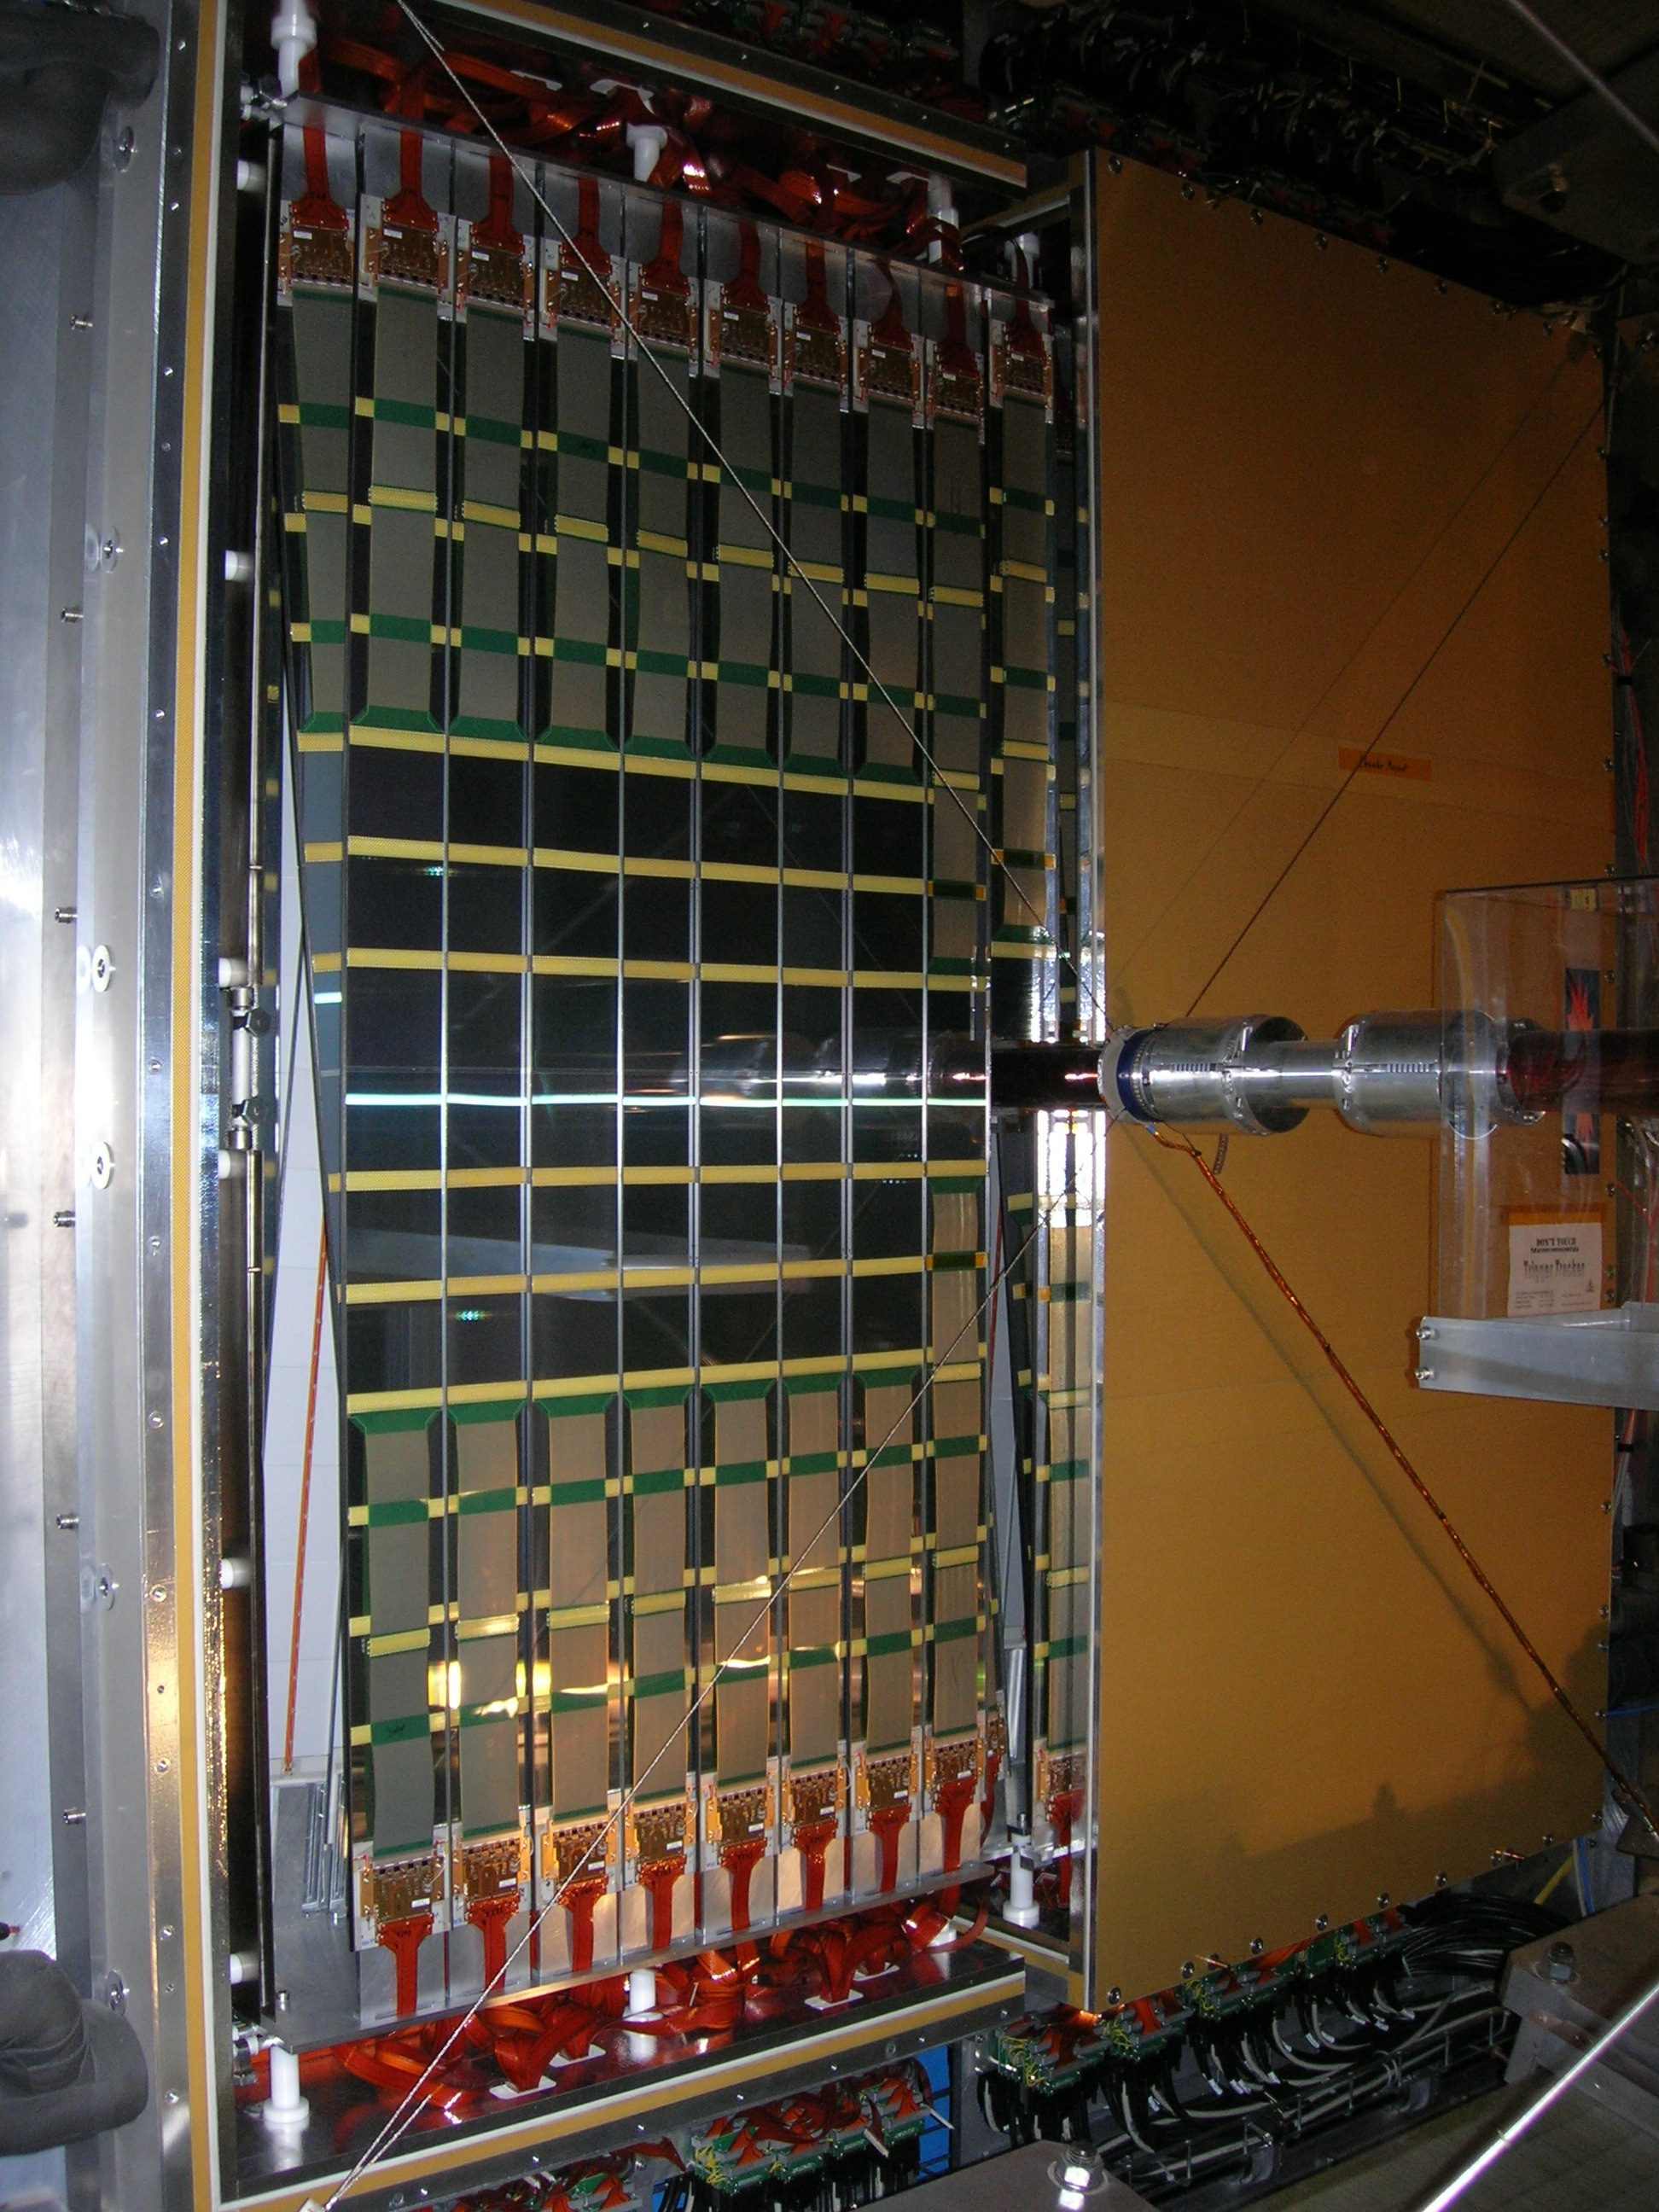
\includegraphics[height=3cm]{Figures Introductory Lecture/LHCb Detector/LHCb_TT.jpg}%source:https://twiki.cern.ch/twiki/bin/view/LHCb/ConferenceSummaryIEEFlorida2009
        \end{figure}
    \end{minipage}
    \vspace{-0.5cm}
    \begin{figure}[h]
    \centering
    \begin{overpic}[width=0.8\textwidth]{Figures Introductory Lecture/LHCb Detector/LHCb_3.png}
           
        \put (20,40) {\rotatebox[]{90}{\colorbox{LHCbDarkBlue!80}{\textcolor{LHCbLightBlue}{\centering \tiny  TT}}}}
        \put (13,45) {\colorbox{lightgray}{\centering \tiny  RICH 1}}
        \put (3,35) {\colorbox{lightgray}{\centering \tiny  VELO}}

\put (1,5) {\tiny $z/m \rightarrow$}
\put (17.5,2) {\tiny $2$}
\put (21.4,2) {\tiny $3$}

    \end{overpic}
    \end{figure}
\end{frame}

\begin{frame}
    \begin{figure}[h]
        \centering
        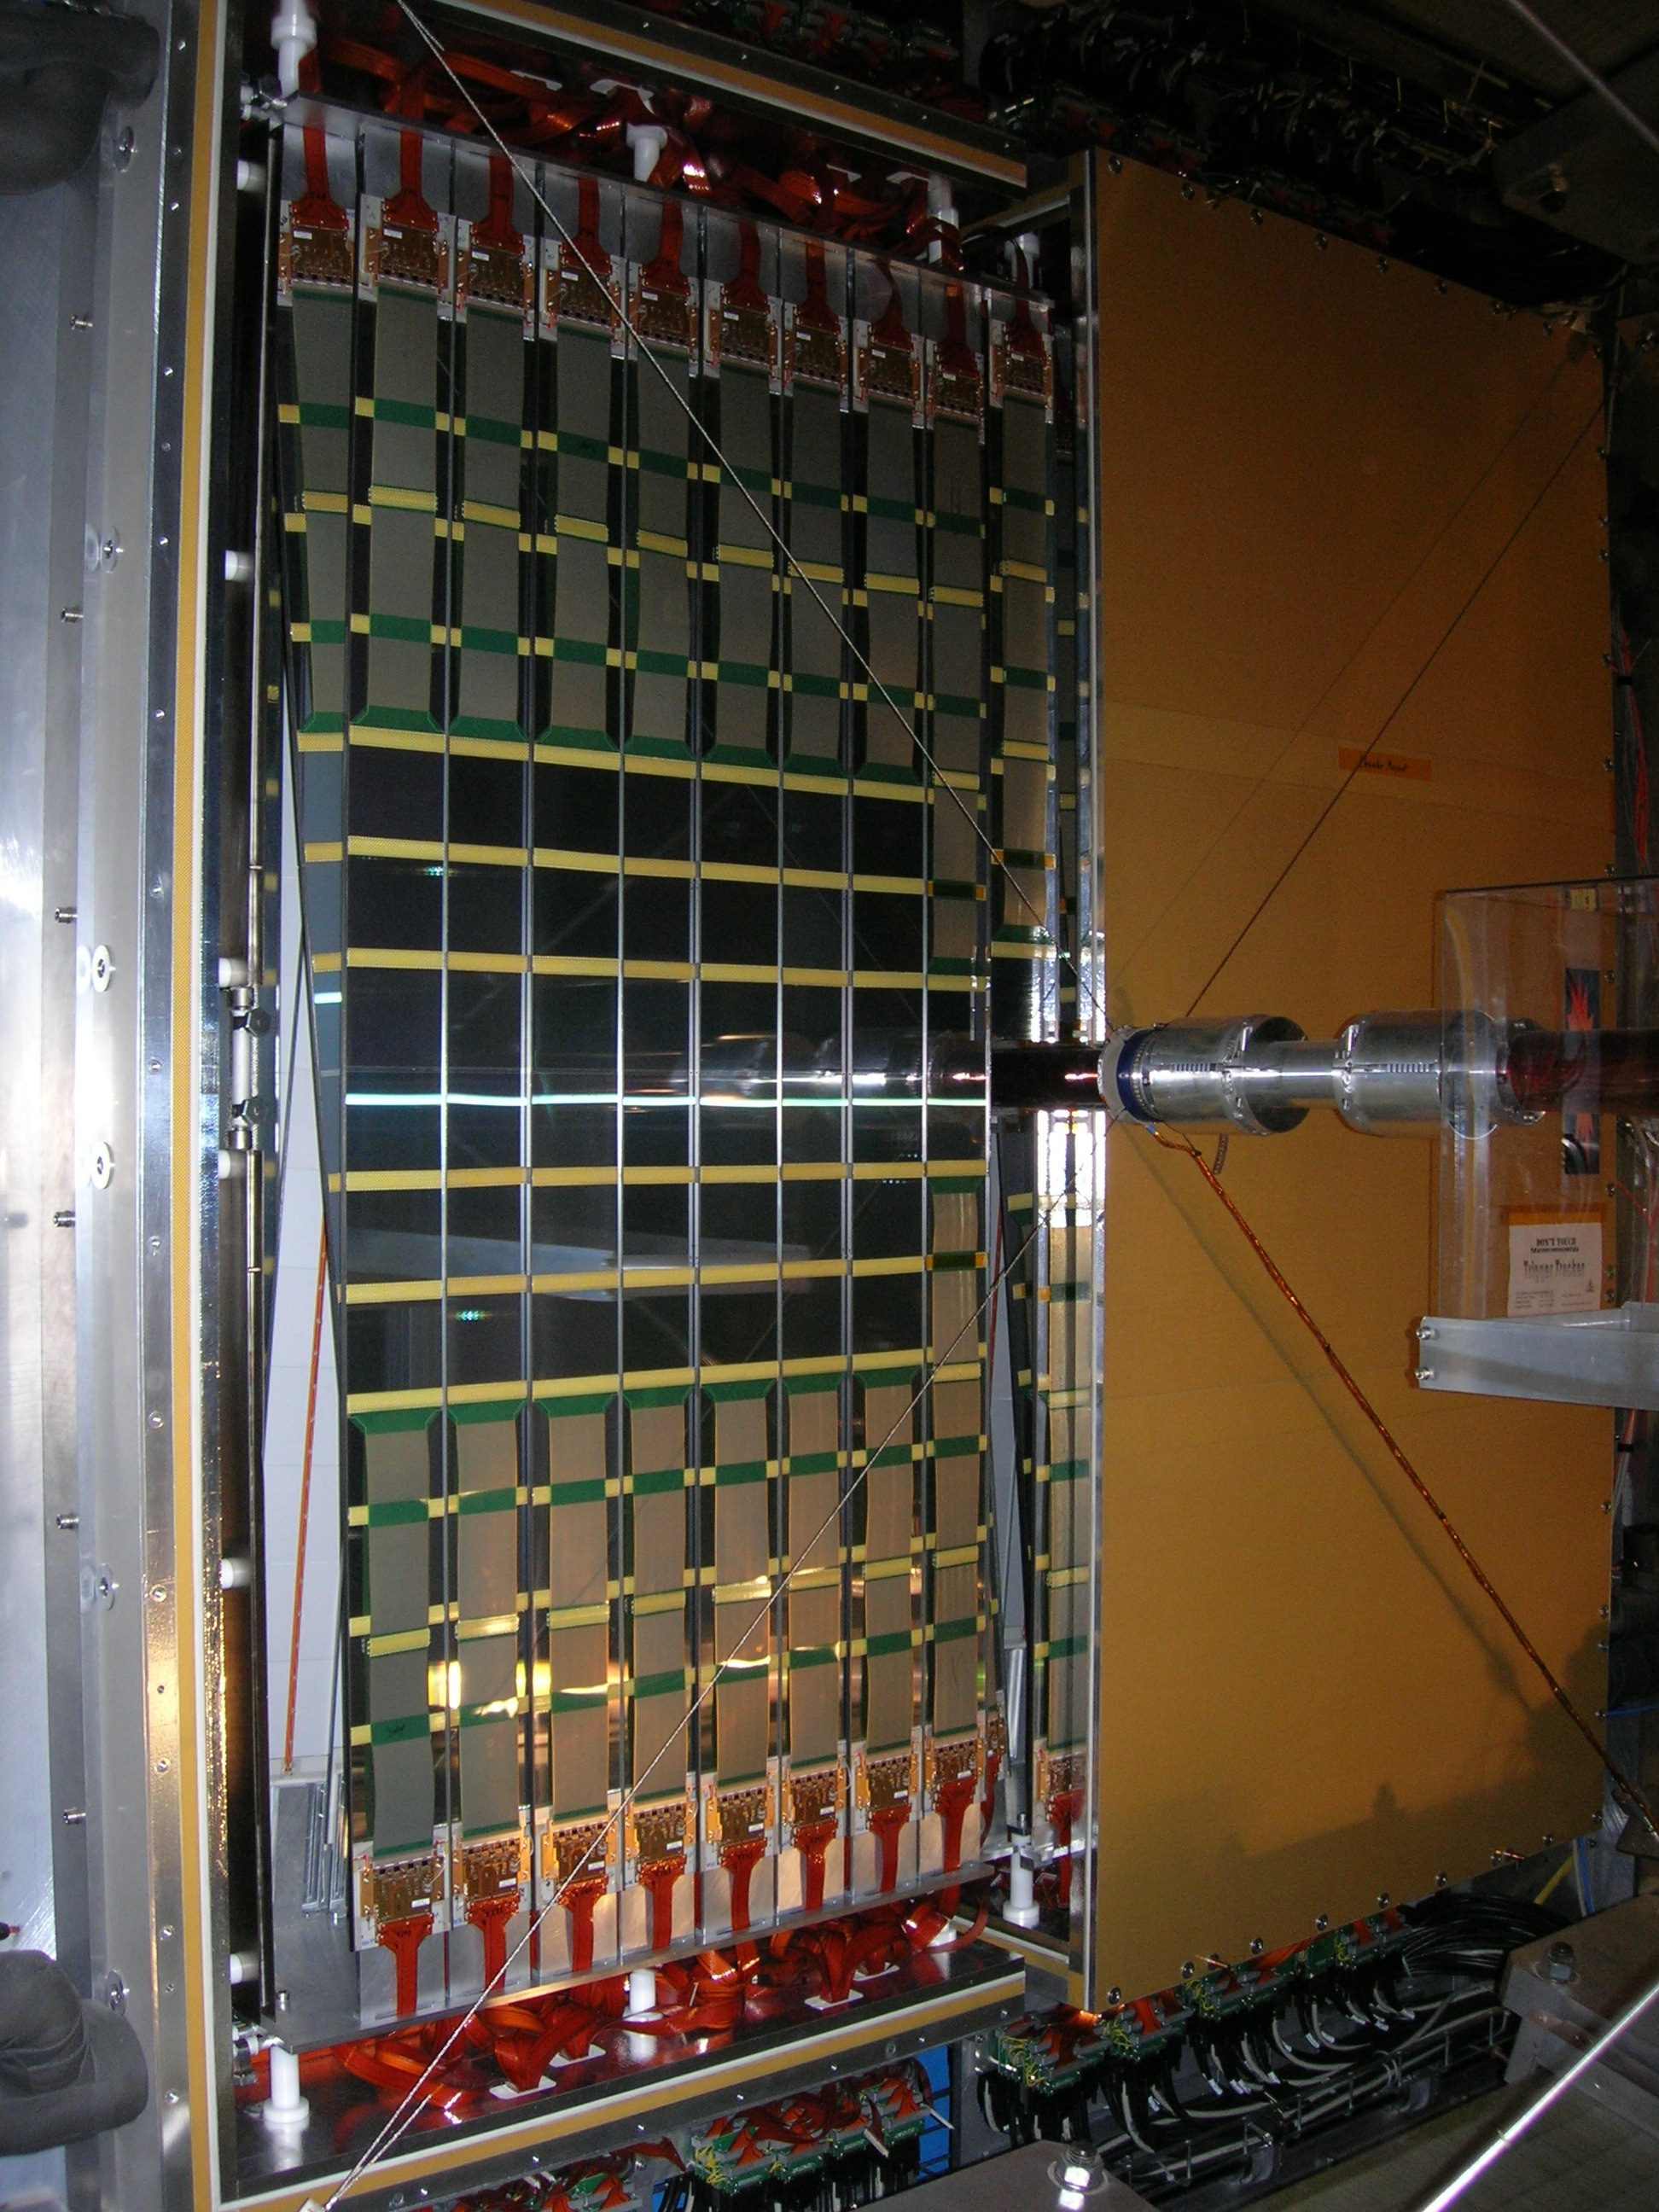
\includegraphics[height=\textheight]{Figures Introductory Lecture/LHCb Detector/LHCb_TT.jpg}%source:https://twiki.cern.ch/twiki/bin/view/LHCb/ConferenceSummaryIEEFlorida2009
        \end{figure}
\end{frame}
%%%%%%%%%%%%%%%%%%%%%%%%%%%%%%%%%%%%%%%%%%%%%%%%%%%%%%%%%%%%%%%%%%%%%%%%%%%%%%%%%%%%%%%%%%%%%%
\begin{frame}{Magnet}
    \begin{minipage}{0.58\textwidth}
    \begin{itemize}
        \item Krümmt die Flugbahn der Teilchen proportional zum \textcolor{red}{\textbf{Impuls}} und \textcolor{red}{\textbf{el. Ladung}} 
        \item Hilft Teilchen zu identifizieren %hier evtl. SuS fragen wieso?
    \end{itemize}
    \end{minipage}\hfill
    \begin{minipage}{0.38\textwidth}
        \begin{figure}[h]
        \centering
        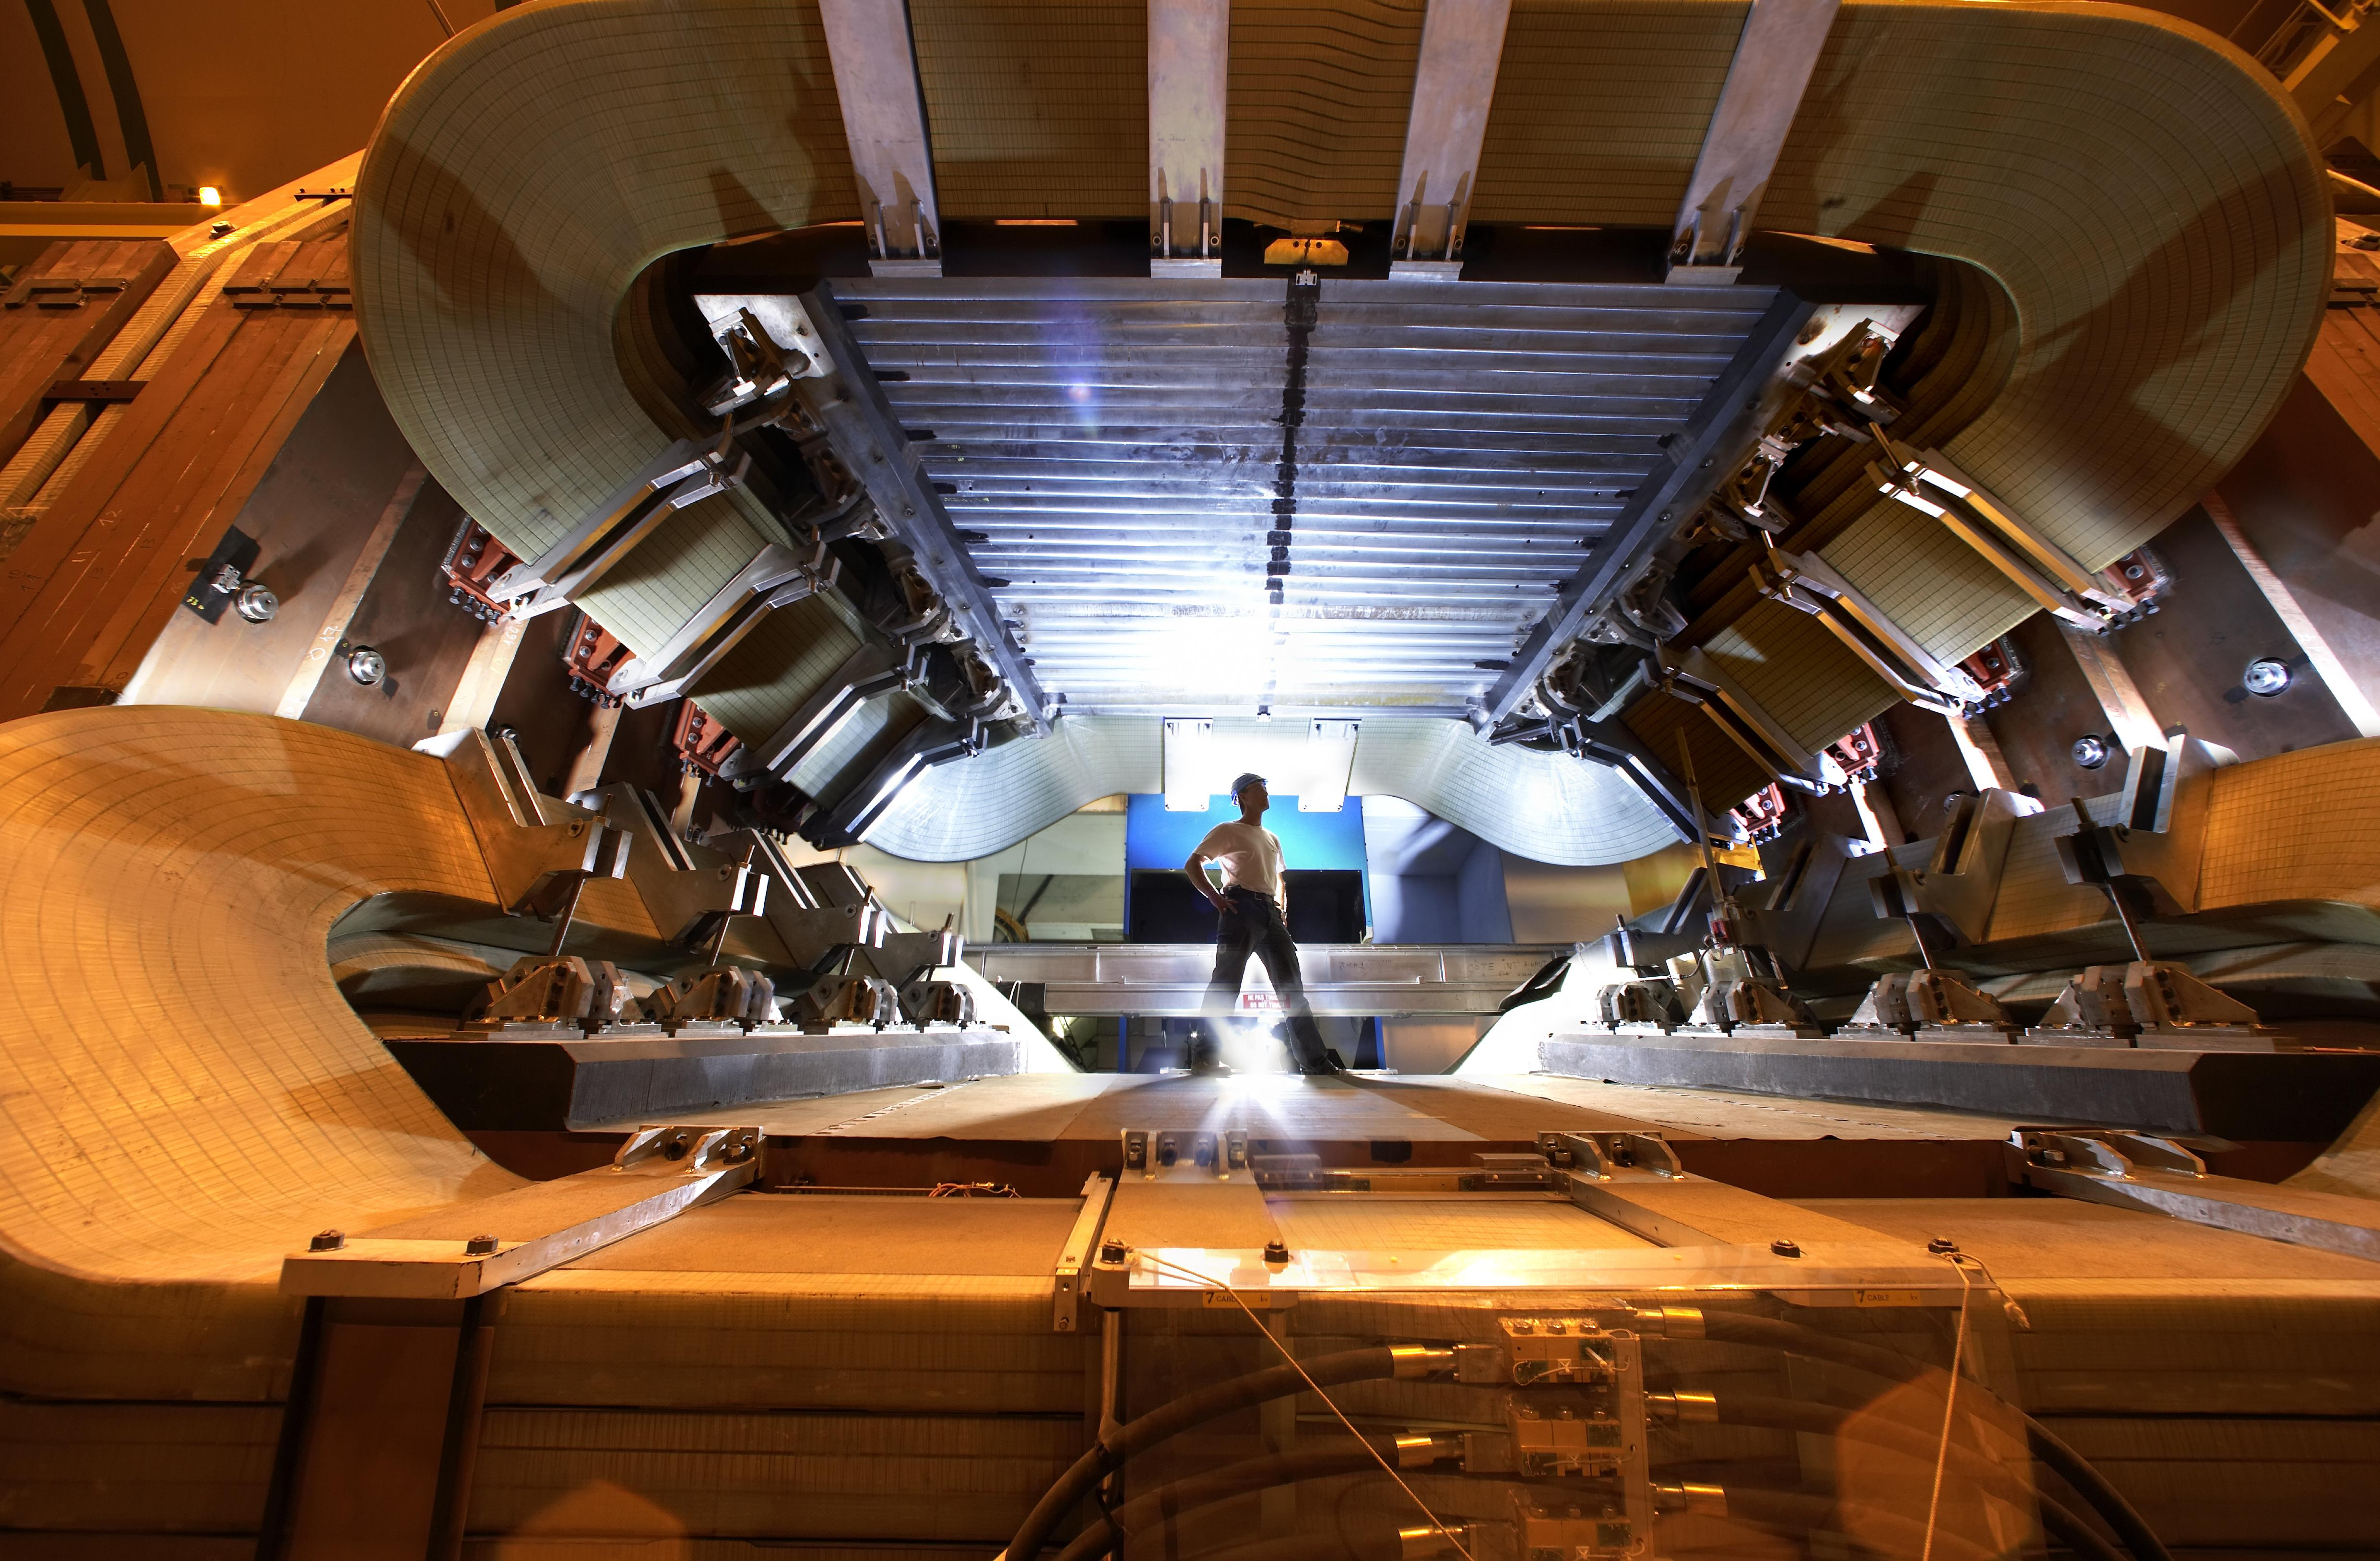
\includegraphics[height=3cm]{Figures Introductory Lecture/LHCb Detector/LHCb_Magnet.jpg}%source:https://cds.cern.ch/record/1124307
        \end{figure}
    \end{minipage}
    \vspace{-0.5cm}
    \begin{figure}[h]
    \centering
    \begin{overpic}[width=0.8\textwidth]{Figures Introductory Lecture/LHCb Detector/LHCb_4.png}
         
        \put (27,52) {\colorbox{LHCbDarkBlue!80}{\textcolor{LHCbLightBlue}{\centering \tiny  Magnet}}}
        \put (20,40) {\rotatebox[]{90}{\colorbox{lightgray}{\centering \tiny  TT}}}
        \put (13,45) {\colorbox{lightgray}{\centering \tiny  RICH 1}}
        \put (3,35) {\colorbox{lightgray}{\centering \tiny  VELO}}

\put (1,5) {\tiny $z/m \rightarrow$}
\put (17.5,2) {\tiny $2$}
\put (21.4,2) {\tiny $3$}
\put (25.5,2) {\tiny $4$}

    
    \end{overpic}
    \end{figure}
\end{frame}
\begin{frame}
    \begin{figure}[h]
        \centering
        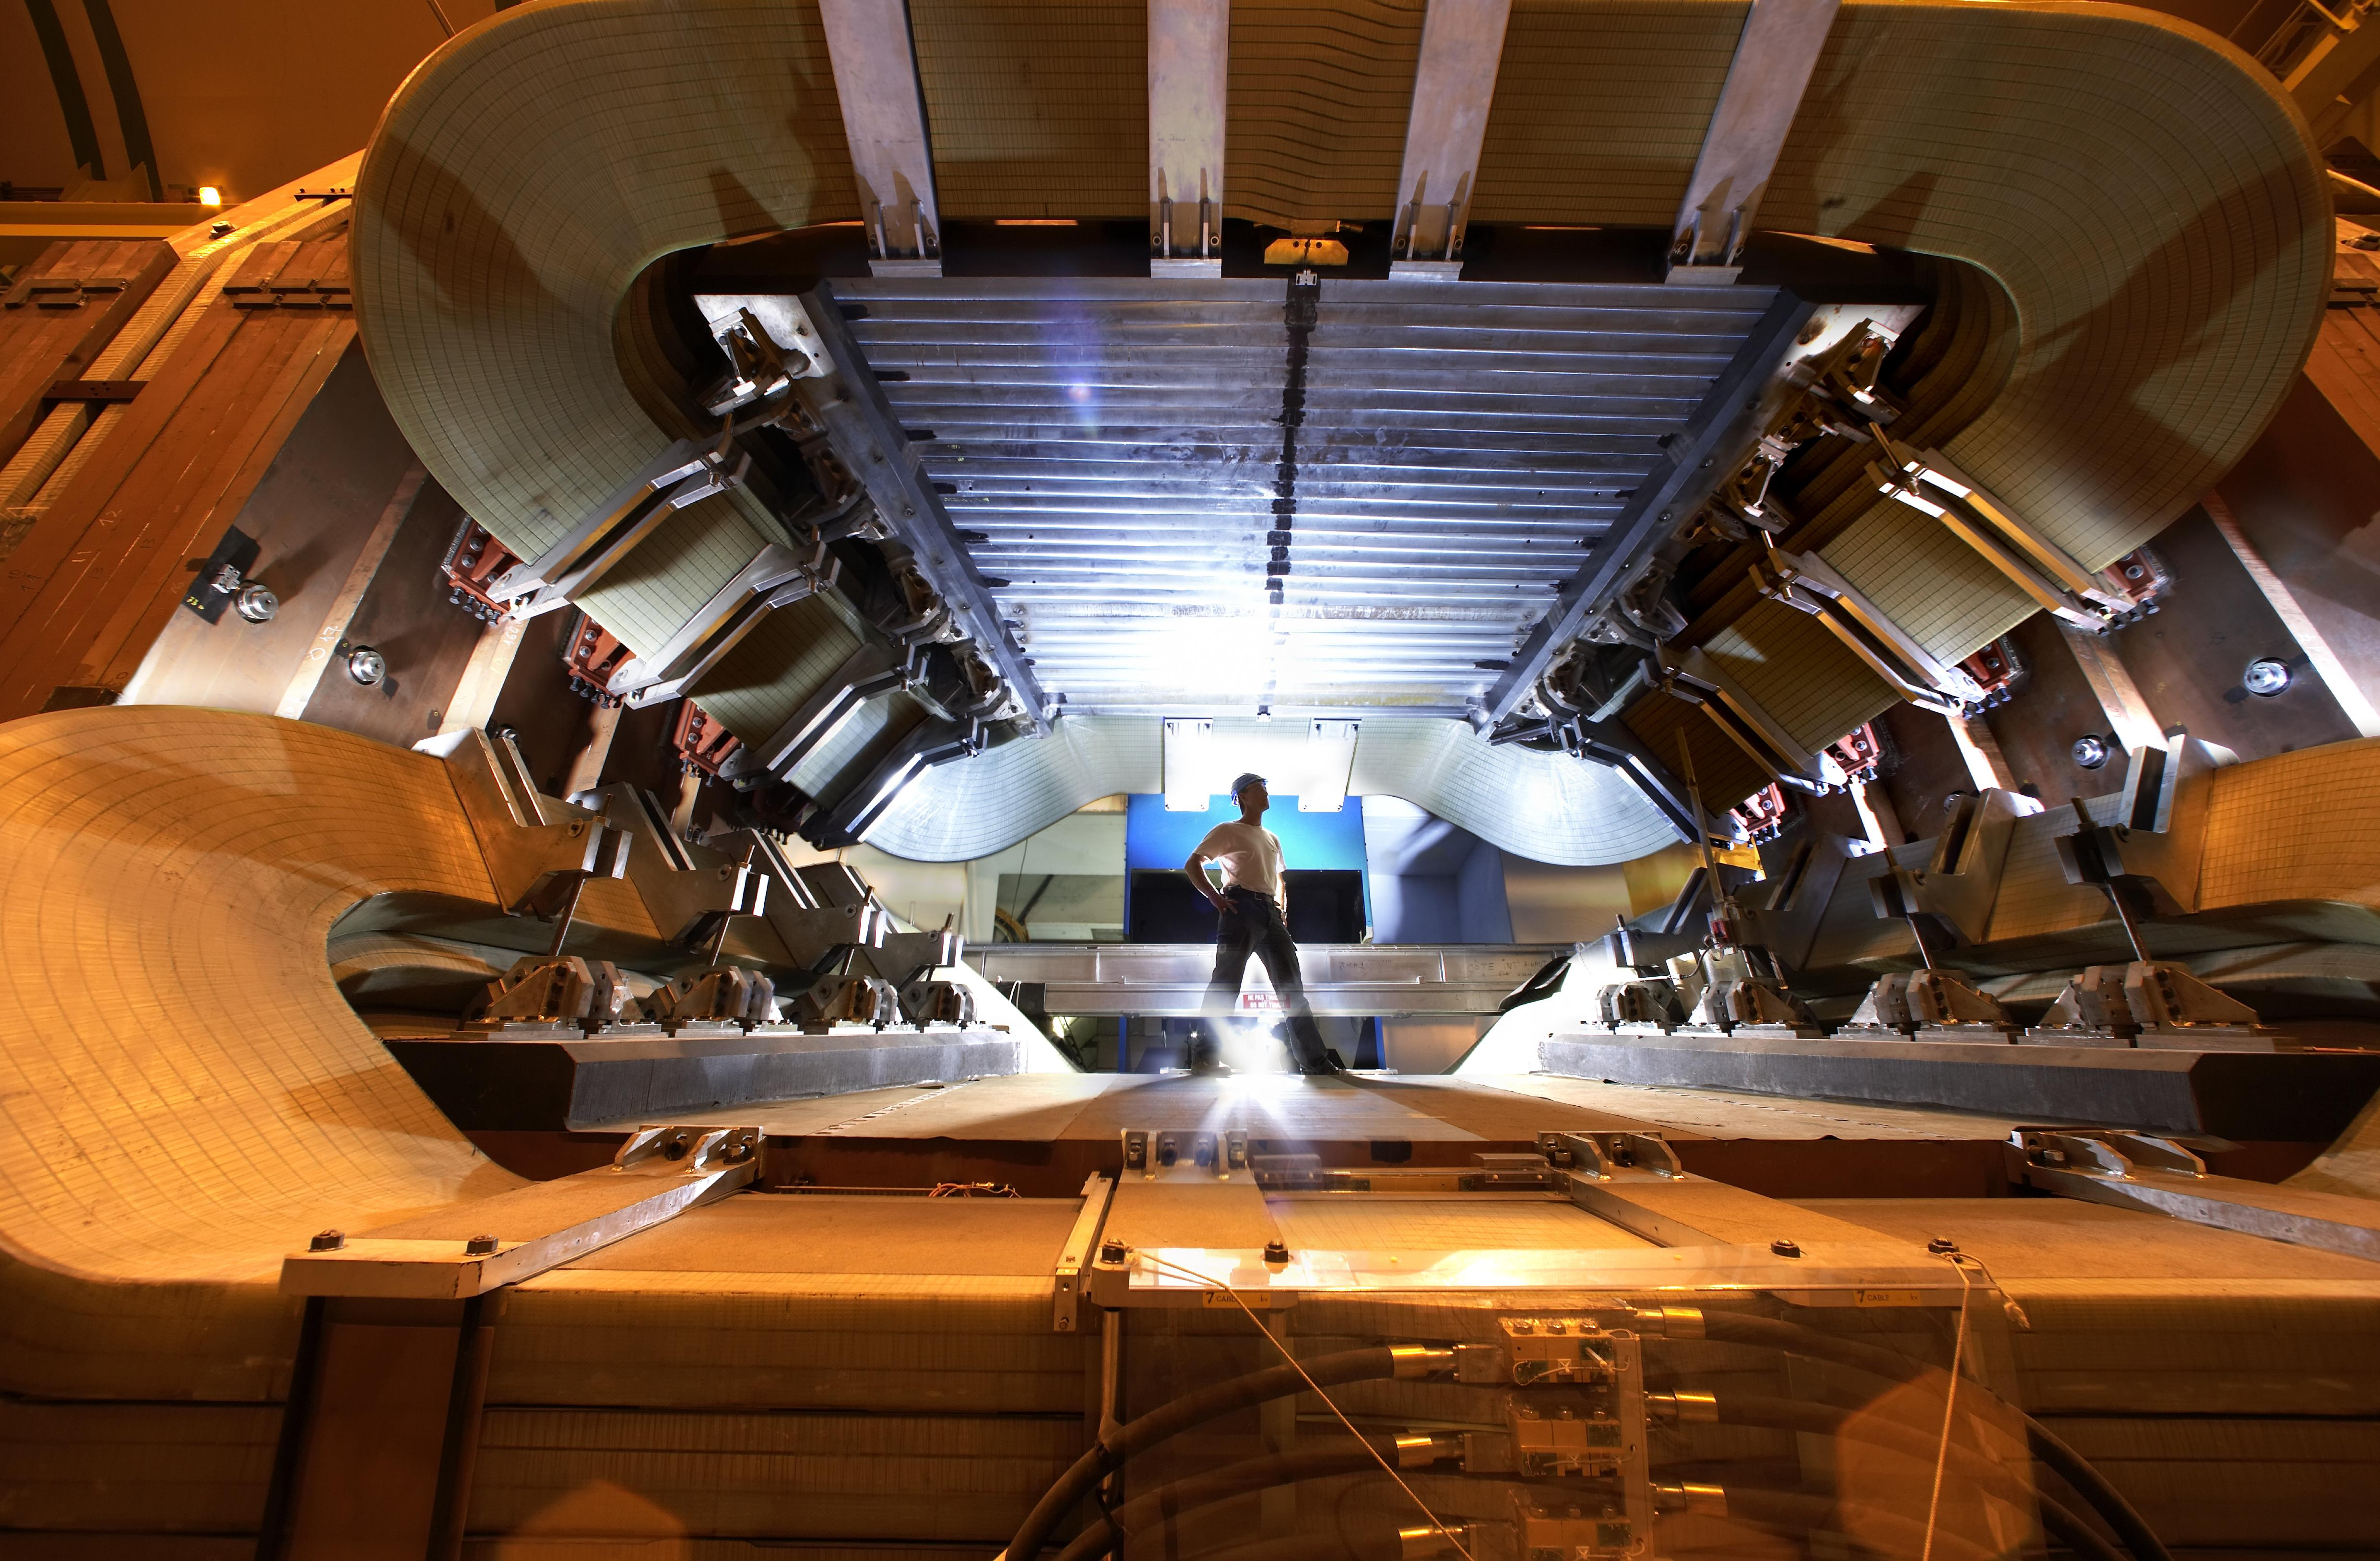
\includegraphics[width=\textwidth]{Figures Introductory Lecture/LHCb Detector/LHCb_Magnet.jpg}%source:https://cds.cern.ch/record/1124307
        \end{figure}
\end{frame}
\begin{frame}{Magnet}
Was passiert mit Teilchen in einem magnetischen Feld?
\begin{minipage}{.39\textwidth} 
Lorentzkraft:
\begin{align*}
    \Vec{F_L}&=q\cdot(\Vec{v}\times\Vec{B}) \\
    F_L&=qvB
\end{align*}
Zentrifugalkraft: %fundamental formular with vectors too irritating!
\begin{align*}
 F_Z&=m \frac{v^2}{r}
\end{align*}
Gleichsetzen: 
\begin{align*}
 qvB&=m \frac{v^2}{r} \\
 \Rightarrow~~ r&=\frac{mv}{qB}=\frac{p}{qB}
\end{align*}

\end{minipage}
\begin{minipage}{.59\textwidth}
    

    \begin{tikzpicture}[scale=1,rotate=-90]     \clip (-6,-6.5) rectangle (0.5,0.5); % Ausschnitt definieren
\draw[](-3,-3)circle(0.141cm);
    \draw[--] (-3.1,-3.1)--(-2.9,-2.9);
    \draw[--] (-3.1,-2.9)--(-2.9,-3.1);


\draw[](-2,-3)circle(0.141cm);
    \draw[--] (-2.1,-3.1)--(-1.9,-2.9);
    \draw[--] (-2.1,-2.9)--(-1.9,-3.1);

\draw[](-1,-3)circle(0.141cm);
    \draw[--] (-1.1,-3.1)--(-0.9,-2.9);
    \draw[--] (-1.1,-2.9)--(-0.9,-3.1);

\draw[](-3,-2)circle(0.141cm);
    \draw[--] (-3.1,-2.1)--(-2.9,-1.9);
    \draw[--] (-3.1,-1.9)--(-2.9,-2.1);

\draw[] (-2,-2) node {$\Vec{B}$};
% \draw[](-2,-2)circle(0.141cm);
%     \draw[--] (-2.1,-2.1)--(-1.9,-1.9);
%     \draw[--] (-2.1,-1.9)--(-1.9,-2.1);

\draw[](-1,-2)circle(0.141cm);
    \draw[--] (-1.1,-2.1)--(-0.9,-1.9);
    \draw[--] (-1.1,-1.9)--(-0.9,-2.1);

\draw[](-3,-1)circle(0.141cm);
    \draw[--] (-3.1,-1.1)--(-2.9,-0.9);
    \draw[--] (-3.1,-0.9)--(-2.9,-1.1);

\draw[](-2,-1)circle(0.141cm);
    \draw[--] (-2.1,-1.1)--(-1.9,-0.9);
    \draw[--] (-2.1,-0.9)--(-1.9,-1.1);

 \draw[](-1,-1)circle(0.141cm);
    \draw[--] (-1.1,-1.1)--(-0.9,-0.9);
    \draw[--] (-1.1,-0.9)--(-0.9,-1.1);

\draw[](-3,-4)circle(0.141cm);
    \draw[--] (-3.1,-4.1)--(-2.9,-3.9);
    \draw[--] (-3.1,-3.9)--(-2.9,-4.1);

\draw[](-2,-4)circle(0.141cm);
    \draw[--] (-2.1,-4.1)--(-1.9,-3.9);
    \draw[--] (-2.1,-3.9)--(-1.9,-4.1);

 \draw[](-1,-4)circle(0.141cm);
    \draw[--] (-1.1,-4.1)--(-0.9,-3.9);
    \draw[--] (-1.1,-3.9)--(-0.9,-4.1);

 \draw[](-4,-4)circle(0.141cm);
    \draw[--] (-4.1,-4.1)--(-3.9,-3.9);
    \draw[--] (-4.1,-3.9)--(-3.9,-4.1);

    \draw[](-4,-3)circle(0.141cm);
    \draw[--] (-4.1,-3.1)--(-3.9,-2.9);
    \draw[--] (-4.1,-2.9)--(-3.9,-3.1);

\draw[](-4,-2)circle(0.141cm);
    \draw[--] (-4.1,-2.1)--(-3.9,-1.9);
    \draw[--] (-4.1,-1.9)--(-3.9,-2.1);

\draw[](-4,-1)circle(0.141cm);
    \draw[--] (-4.1,-1.1)--(-3.9,-0.9);
    \draw[--] (-4.1,-0.9)--(-3.9,-1.1);


 \draw[](-5,-4)circle(0.141cm);
    \draw[--] (-5.1,-4.1)--(-4.9,-3.9);
    \draw[--] (-5.1,-3.9)--(-4.9,-4.1);

    \draw[](-5,-3)circle(0.141cm);
    \draw[--] (-5.1,-3.1)--(-4.9,-2.9);
    \draw[--] (-5.1,-2.9)--(-4.9,-3.1);

\draw[](-5,-2)circle(0.141cm);
    \draw[--] (-5.1,-2.1)--(-4.9,-1.9);
    \draw[--] (-5.1,-1.9)--(-4.9,-2.1);

\draw[](-5,-1)circle(0.141cm);
    \draw[--] (-5.1,-1.1)--(-4.9,-0.9);
    \draw[--] (-5.1,-0.9)--(-4.9,-1.1);


    \draw[](-5,-5)circle(0.141cm);
    \draw[--] (-5.1,-5.1)--(-4.9,-4.9);
    \draw[--] (-5.1,-4.9)--(-4.9,-5.1);

        \draw[](-4,-5)circle(0.141cm);
    \draw[--] (-4.1,-5.1)--(-3.9,-4.9);
    \draw[--] (-4.1,-4.9)--(-3.9,-5.1);

            \draw[](-3,-5)circle(0.141cm);
    \draw[--] (-3.1,-5.1)--(-2.9,-4.9);
    \draw[--] (-3.1,-4.9)--(-2.9,-5.1);

            \draw[](-2,-5)circle(0.141cm);
    \draw[--] (-2.1,-5.1)--(-1.9,-4.9);
    \draw[--] (-2.1,-4.9)--(-1.9,-5.1);

            \draw[](-1,-5)circle(0.141cm);
    \draw[--] (-1.1,-5.1)--(-0.9,-4.9);
    \draw[--] (-1.1,-4.9)--(-0.9,-5.1);

 \draw[blue,line width=2pt] (-0.65,-2.3) --++ (90:0)  arc (90:180:3)   ;
 \draw[->, blue,line width=2pt] (-0.65,-2.3)--(-0.5,-2.3)node[black,right] {$e^-$};
 \draw  (-0.8,-5.2) circle (1pt) ;
 \draw[--,dashed] (-0.8,-5.2) to node [right] {$r$}(-2.5,-3){};
\node at (-6,-6){};
\end{tikzpicture}\end{minipage}
\end{frame}
\subsection{}
\begin{frame}{Magnet}
Um welche Teilchen könnte es sich handeln?
\begin{minipage}{.39\textwidth} 
\begin{align*}
 r=\frac{mv}{qB}=\frac{p}{qB}
\end{align*} \\ Kann es eines der folgenden sein?\begin{itemize}
    \item  $p$
    \item  $e^-$
    \item  $e^+$ 
    \item  $n$
    \item  $\gamma$
    \item  $H$
\end{itemize}

\end{minipage}
\begin{minipage}{.59\textwidth}
    

    \begin{tikzpicture}[scale=1,rotate=-90]
     \clip (-6,-6.5) rectangle (0.5,0.5); % Ausschnitt definieren
\draw[](-3,-3)circle(0.141cm);
    \draw[--] (-3.1,-3.1)--(-2.9,-2.9);
    \draw[--] (-3.1,-2.9)--(-2.9,-3.1);


\draw[](-2,-3)circle(0.141cm);
    \draw[--] (-2.1,-3.1)--(-1.9,-2.9);
    \draw[--] (-2.1,-2.9)--(-1.9,-3.1);

\draw[](-1,-3)circle(0.141cm);
    \draw[--] (-1.1,-3.1)--(-0.9,-2.9);
    \draw[--] (-1.1,-2.9)--(-0.9,-3.1);

\draw[](-3,-2)circle(0.141cm);
    \draw[--] (-3.1,-2.1)--(-2.9,-1.9);
    \draw[--] (-3.1,-1.9)--(-2.9,-2.1);

\draw[] (-2,-2) node {$\Vec{B}$};
% \draw[](-2,-2)circle(0.141cm);
%     \draw[--] (-2.1,-2.1)--(-1.9,-1.9);
%     \draw[--] (-2.1,-1.9)--(-1.9,-2.1);

\draw[](-1,-2)circle(0.141cm);
    \draw[--] (-1.1,-2.1)--(-0.9,-1.9);
    \draw[--] (-1.1,-1.9)--(-0.9,-2.1);

\draw[](-3,-1)circle(0.141cm);
    \draw[--] (-3.1,-1.1)--(-2.9,-0.9);
    \draw[--] (-3.1,-0.9)--(-2.9,-1.1);

\draw[](-2,-1)circle(0.141cm);
    \draw[--] (-2.1,-1.1)--(-1.9,-0.9);
    \draw[--] (-2.1,-0.9)--(-1.9,-1.1);

 \draw[](-1,-1)circle(0.141cm);
    \draw[--] (-1.1,-1.1)--(-0.9,-0.9);
    \draw[--] (-1.1,-0.9)--(-0.9,-1.1);

\draw[](-3,-4)circle(0.141cm);
    \draw[--] (-3.1,-4.1)--(-2.9,-3.9);
    \draw[--] (-3.1,-3.9)--(-2.9,-4.1);

\draw[](-2,-4)circle(0.141cm);
    \draw[--] (-2.1,-4.1)--(-1.9,-3.9);
    \draw[--] (-2.1,-3.9)--(-1.9,-4.1);

 \draw[](-1,-4)circle(0.141cm);
    \draw[--] (-1.1,-4.1)--(-0.9,-3.9);
    \draw[--] (-1.1,-3.9)--(-0.9,-4.1);

 \draw[](-4,-4)circle(0.141cm);
    \draw[--] (-4.1,-4.1)--(-3.9,-3.9);
    \draw[--] (-4.1,-3.9)--(-3.9,-4.1);

    \draw[](-4,-3)circle(0.141cm);
    \draw[--] (-4.1,-3.1)--(-3.9,-2.9);
    \draw[--] (-4.1,-2.9)--(-3.9,-3.1);

\draw[](-4,-2)circle(0.141cm);
    \draw[--] (-4.1,-2.1)--(-3.9,-1.9);
    \draw[--] (-4.1,-1.9)--(-3.9,-2.1);

\draw[](-4,-1)circle(0.141cm);
    \draw[--] (-4.1,-1.1)--(-3.9,-0.9);
    \draw[--] (-4.1,-0.9)--(-3.9,-1.1);


 \draw[](-5,-4)circle(0.141cm);
    \draw[--] (-5.1,-4.1)--(-4.9,-3.9);
    \draw[--] (-5.1,-3.9)--(-4.9,-4.1);

    \draw[](-5,-3)circle(0.141cm);
    \draw[--] (-5.1,-3.1)--(-4.9,-2.9);
    \draw[--] (-5.1,-2.9)--(-4.9,-3.1);

\draw[](-5,-2)circle(0.141cm);
    \draw[--] (-5.1,-2.1)--(-4.9,-1.9);
    \draw[--] (-5.1,-1.9)--(-4.9,-2.1);

\draw[](-5,-1)circle(0.141cm);
    \draw[--] (-5.1,-1.1)--(-4.9,-0.9);
    \draw[--] (-5.1,-0.9)--(-4.9,-1.1);


    \draw[](-5,-5)circle(0.141cm);
    \draw[--] (-5.1,-5.1)--(-4.9,-4.9);
    \draw[--] (-5.1,-4.9)--(-4.9,-5.1);

        \draw[](-4,-5)circle(0.141cm);
    \draw[--] (-4.1,-5.1)--(-3.9,-4.9);
    \draw[--] (-4.1,-4.9)--(-3.9,-5.1);

            \draw[](-3,-5)circle(0.141cm);
    \draw[--] (-3.1,-5.1)--(-2.9,-4.9);
    \draw[--] (-3.1,-4.9)--(-2.9,-5.1);

            \draw[](-2,-5)circle(0.141cm);
    \draw[--] (-2.1,-5.1)--(-1.9,-4.9);
    \draw[--] (-2.1,-4.9)--(-1.9,-5.1);

            \draw[](-1,-5)circle(0.141cm);
    \draw[--] (-1.1,-5.1)--(-0.9,-4.9);
    \draw[--] (-1.1,-4.9)--(-0.9,-5.1);

 \def\Co{green!30}\draw[->,\Co,line width=2pt] (-4,-5.5)  to  node[black,left] {\colorbox{\Co}{Nr. 1}}  (-4,-5.1) --++ (-90:0) arc (180:200:-14)   ;
 \def\Co{blue!30}\draw[->,\Co,line width=2pt] (-3,-5.5)  to  node[black,left] {\colorbox{\Co}{Nr. 2}}  (-3,-5.1) --++ (-90:0) arc (180:184.3:-65)   ;
 \def\Co{red!30}\draw[->,\Co,line width=2pt] (-2,-5.5)    to  node[black,left] {\colorbox{\Co}{Nr. 3}}  (-2,-5.1) --++ (90:0) arc (180:160:14)   ;
\node at (-6,-6){};
\end{tikzpicture}\end{minipage}
\end{frame}
%%%%%%%%%%%%%%%%%%%%%%%%%%%%%%%%%%%%%%%%%%%%%%%%%%%%%%%%%%%%%%%%%%%%%%%%%%%%%%%%%%%%%%%%%%%%%%
\begin{frame}{Tracker T1, T2 und T3}
    \begin{minipage}{0.58\textwidth}
    \begin{itemize}
        \item Misst die \textcolor{red}{\textbf{Position}} der Teilchen
        \item Hilft Teilchen zu identifizieren %hier evtl. schüler fragen wie?
    \end{itemize}
    \end{minipage}\hfill
    \begin{minipage}{0.38\textwidth}
        \begin{figure}[h]
        \centering
        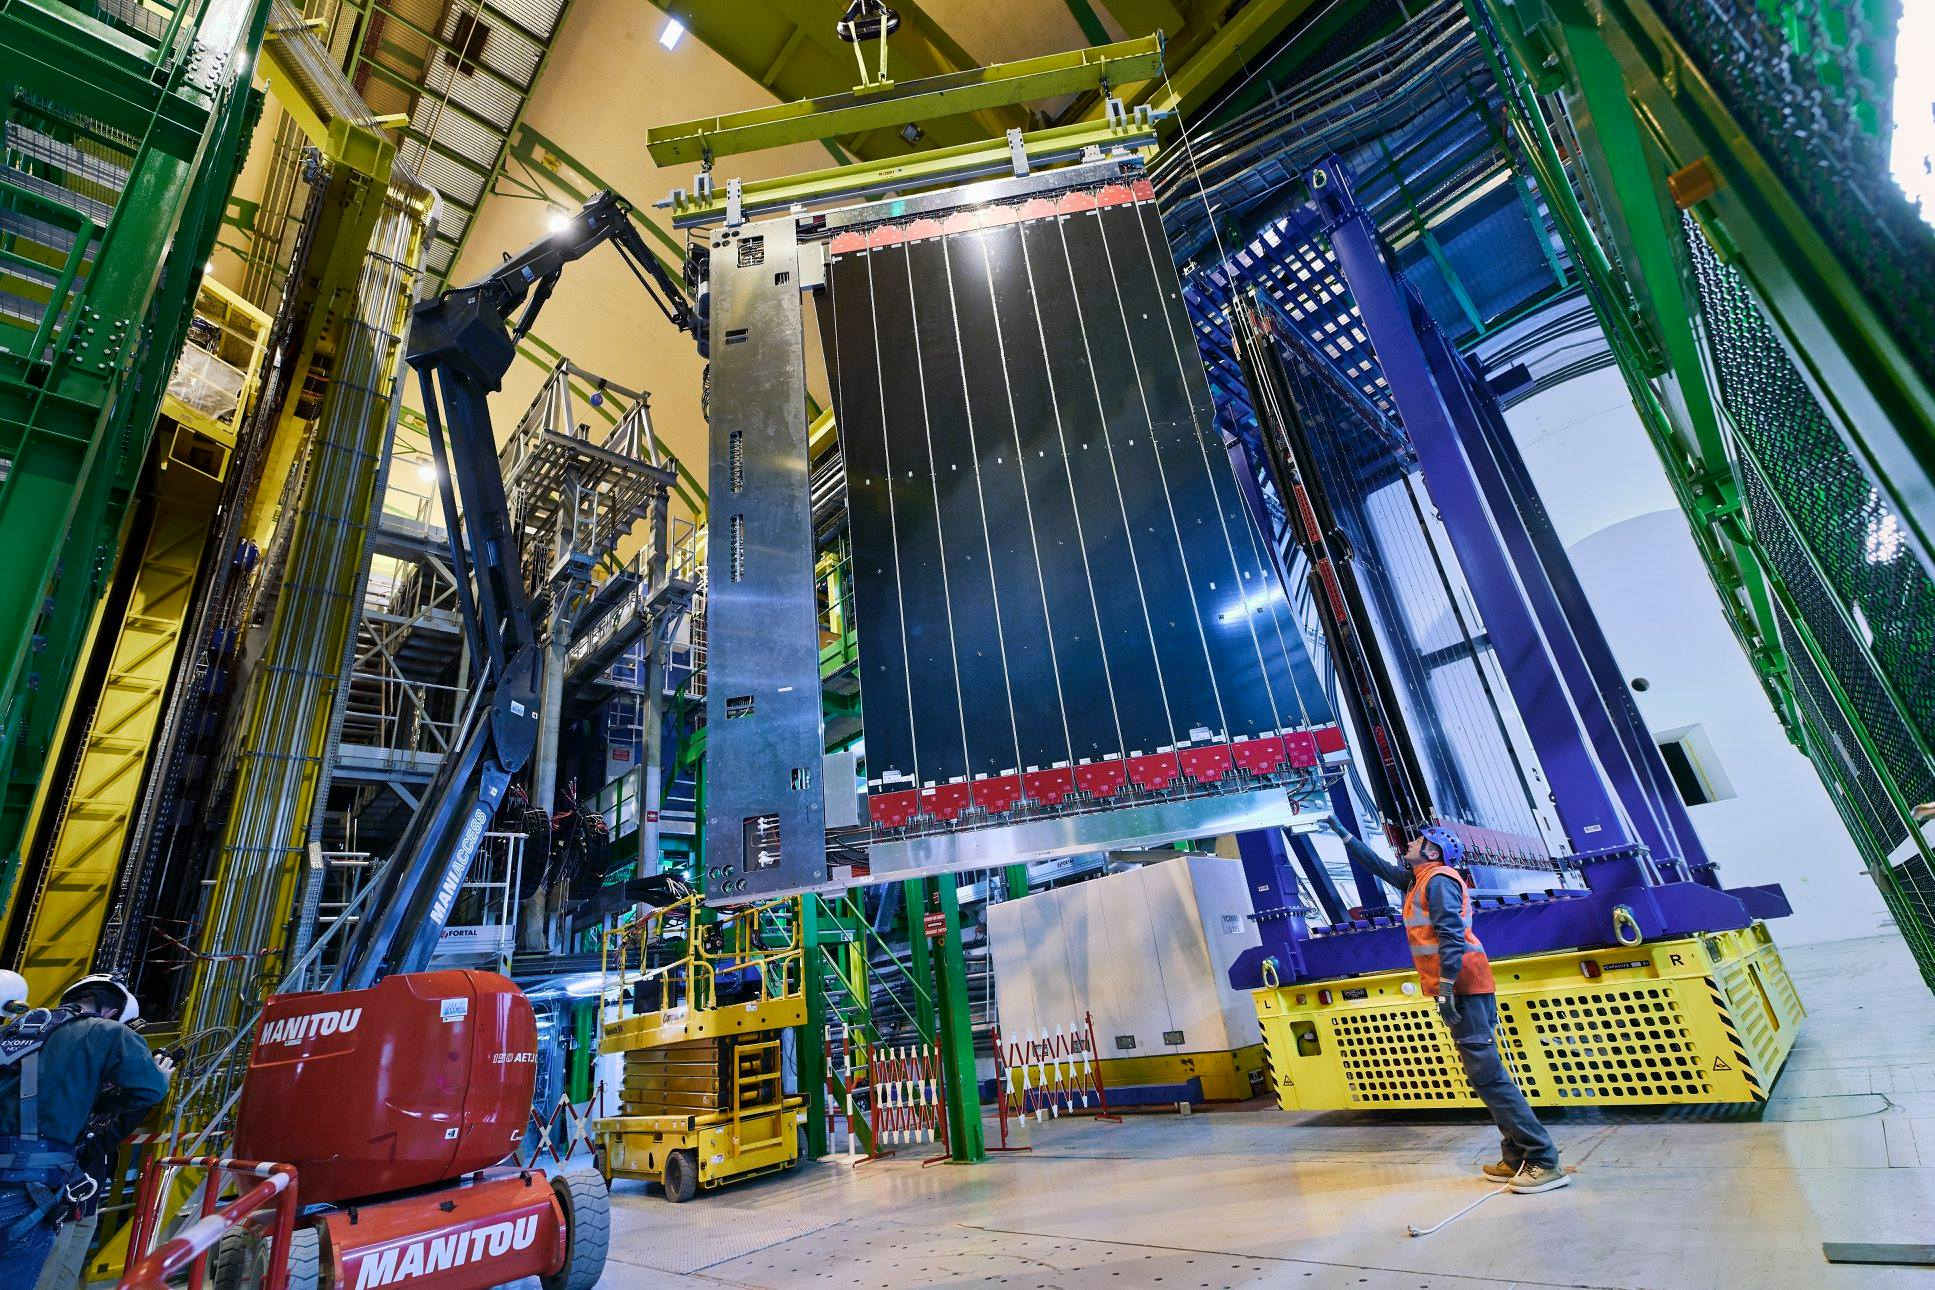
\includegraphics[height=3 cm]{Figures Introductory Lecture/LHCb Detector/LHCb_T1-3.jpg} %source:https://www.facebook.com/LHCbExperiment/photos/a.238680152959433/1123439814483458/?type=3
        \end{figure}
    \end{minipage}
    \vspace{-0.5cm}
    \begin{figure}[h]
    \centering
    \begin{overpic}[width=0.8\textwidth]{Figures Introductory Lecture/LHCb Detector/LHCb_5.png}
          
        \put (42,46) {\rotatebox[]{90}{\colorbox{LHCbDarkBlue!80}{\textcolor{LHCbLightBlue}{\centering \tiny  T1-T3}}}}
        \put (27,52) {\colorbox{lightgray}{\centering \tiny  Magnet}}
        \put (20,40) {\rotatebox[]{90}{\colorbox{lightgray}{\centering \tiny  TT}}}
        \put (13,45) {\colorbox{lightgray}{\centering \tiny  RICH 1}}
        \put (3,35) {\colorbox{lightgray}{\centering \tiny  VELO}}

\put (1,5) {\tiny $z/m \rightarrow$}
\put (17.5,2) {\tiny $2$}
\put (21.4,2) {\tiny $3$}
\put (25.5,2) {\tiny $4$}

\put (39,2) {\tiny $7$}

     
    \end{overpic}
    \end{figure}
\end{frame}
\begin{frame}
     \begin{figure}[h]
        \centering
        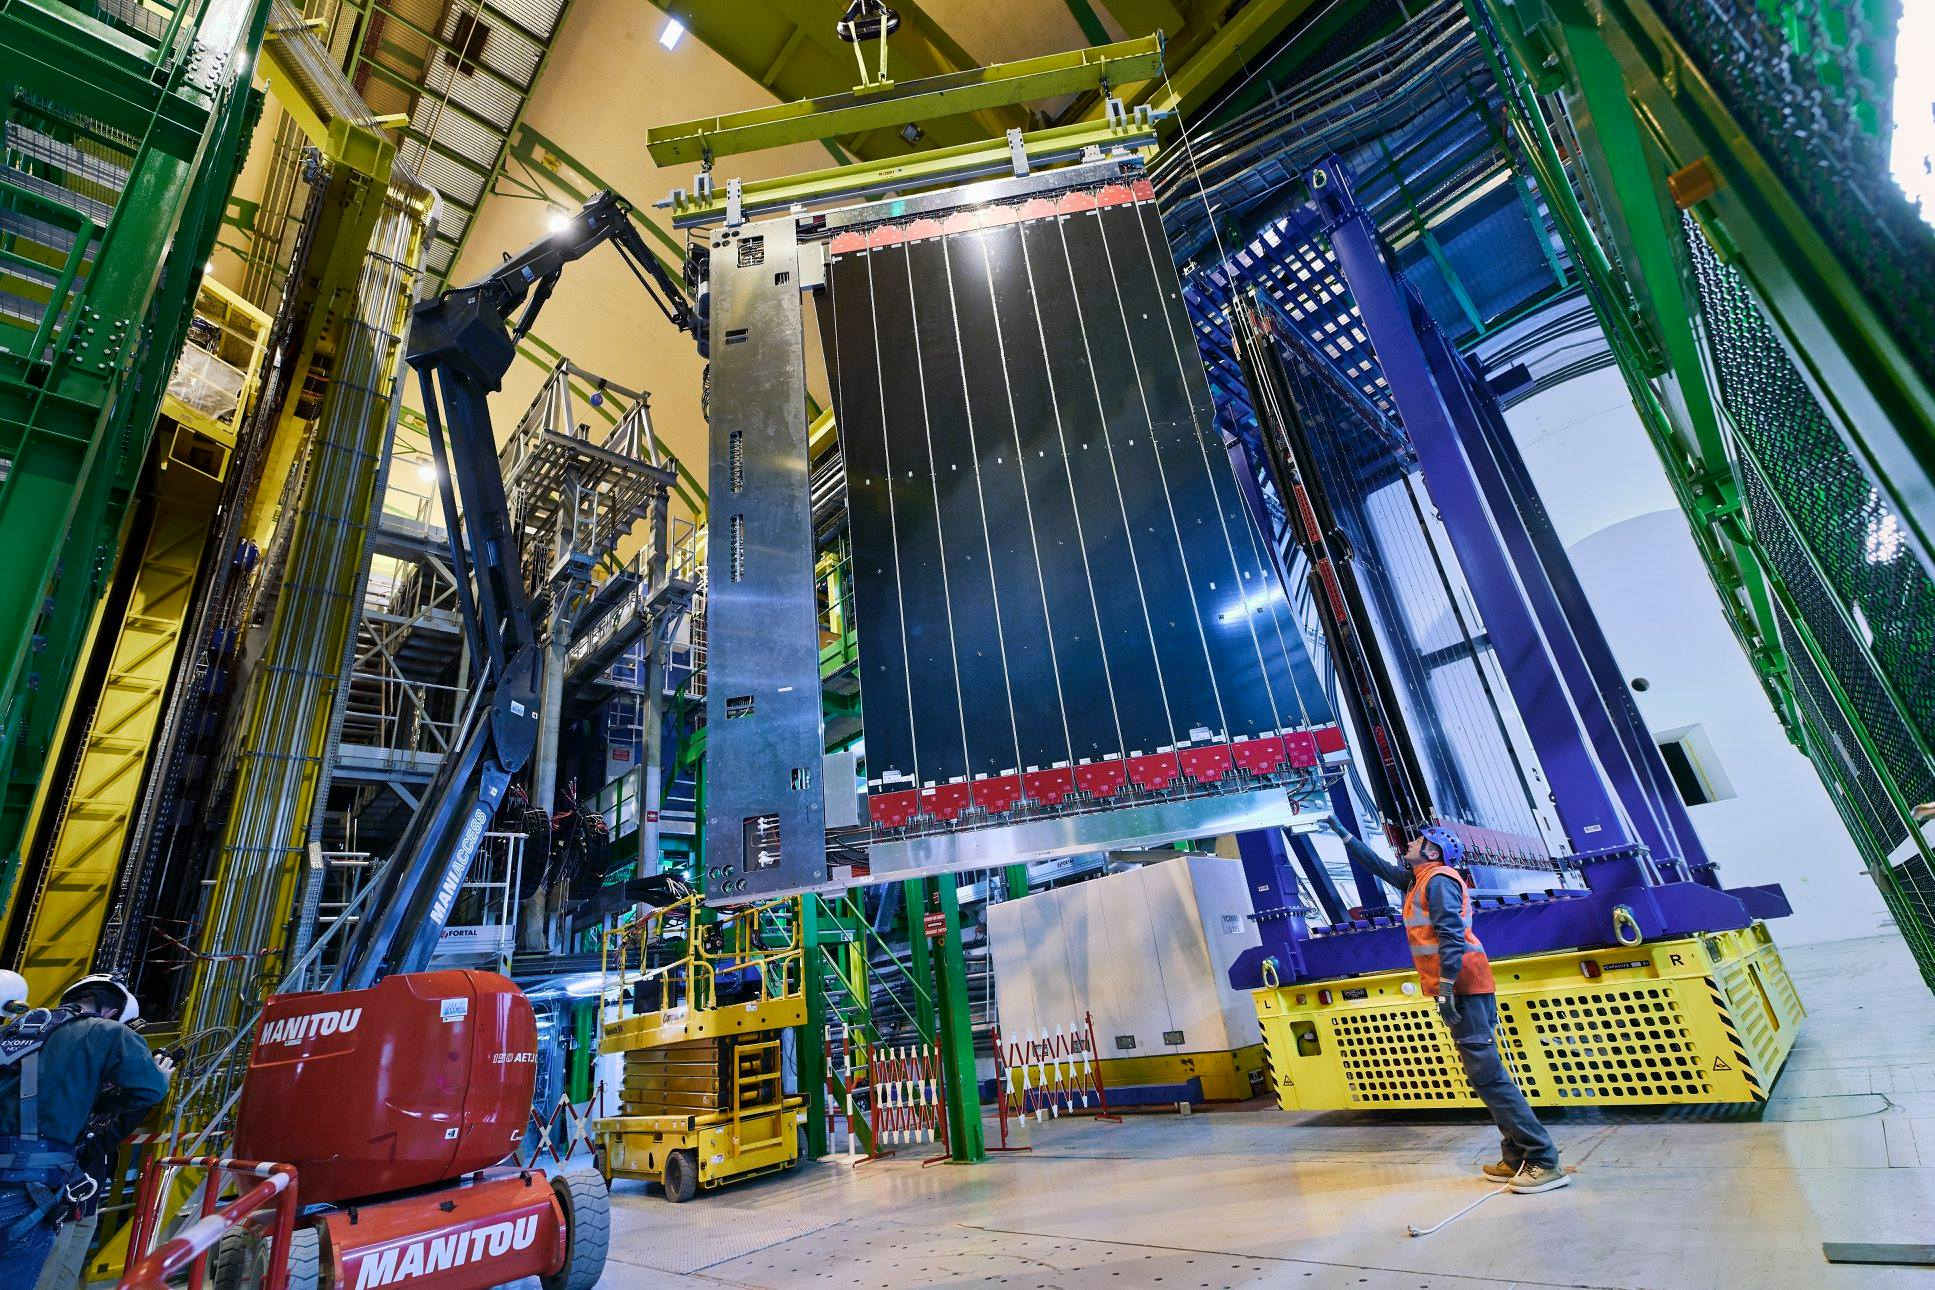
\includegraphics[width=\textwidth]{Figures Introductory Lecture/LHCb Detector/LHCb_T1-3.jpg} %source:https://www.facebook.com/LHCbExperiment/photos/a.238680152959433/1123439814483458/?type=3
        \end{figure}
\end{frame}
%%%%%%%%%%%%%%%%%%%%%%%%%%%%%%%%%%%%%%%%%%%%%%%%%%%%%%%%%%%%%%%%%%%%%%%%%%%%%%%%%%%%%%%%%%%%%%
\begin{frame}{Ring Imaging Cherenkov Detector (RICH2)}
    \begin{minipage}{0.58\textwidth}
    \begin{itemize}
        \item Funktioniert wie RICH1
        \item Nutzt anderes Medium \ding{220} genau in anderem Geschwindigkeitsfenster
    \end{itemize}
    \end{minipage}\hfill
    \begin{minipage}{0.38\textwidth}
        \begin{figure}[h]
        \centering
        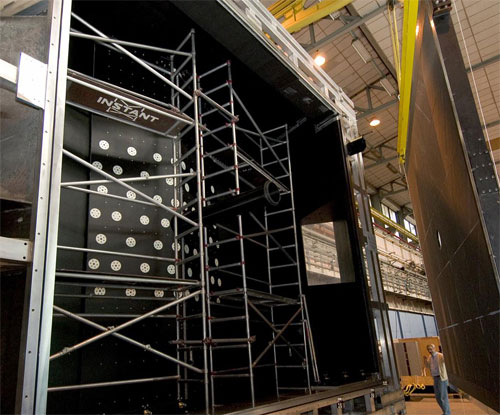
\includegraphics[height=3cm]{Figures Introductory Lecture/LHCb Detector/LHCb_RICH2.jpg}%source:https://www.lhc-facts.ch/index.php?page=lhcb dort wird als quelle cern genannt
        \end{figure}
    \end{minipage}
    \vspace{-0.5cm}
    \begin{figure}[h]
    \centering
    \begin{overpic}[width=0.8\textwidth]{Figures Introductory Lecture/LHCb Detector/LHCb_6.png}
         
        \put (45.3,52) {\colorbox{LHCbDarkBlue!80}{\textcolor{LHCbLightBlue}{\centering \tiny  RICH 2}}}
        \put (42,46) {\rotatebox[]{90}{\colorbox{lightgray}{\centering \tiny  T1-T3}}}
        \put (27,52) {\colorbox{lightgray}{\centering \tiny  Magnet}}
        \put (20,40) {\rotatebox[]{90}{\colorbox{lightgray}{\centering \tiny  TT}}}
        \put (13,45) {\colorbox{lightgray}{\centering \tiny  RICH 1}}
        \put (3,35) {\colorbox{lightgray}{\centering \tiny  VELO}}

\put (1,5) {\tiny $z/m \rightarrow$}
\put (17.5,2) {\tiny $2$}
\put (21.4,2) {\tiny $3$}
\put (25.5,2) {\tiny $4$}

\put (39,2) {\tiny $7$}

\put (50,2) {\tiny $10$}
       
    \end{overpic}
    \end{figure}
\end{frame}
\begin{frame}
    \begin{figure}[h]
        \centering
        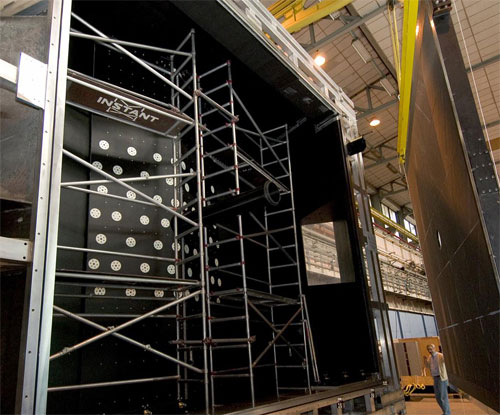
\includegraphics[height=\textheight]{Figures Introductory Lecture/LHCb Detector/LHCb_RICH2.jpg}%source:https://www.lhc-facts.ch/index.php?page=lhcb dort wird als quelle cern genannt
        \end{figure}
\end{frame}
%%%%%%%%%%%%%%%%%%%%%%%%%%%%%%%%%%%%%%%%%%%%%%%%%%%%%%%%%%%%%%%%%%%%%%%%%%%%%%%%%%%%%%%%%%%%%%
\begin{frame}{Elektromagnetisches Kalorimeter (ECAL)}
    \begin{minipage}{0.58\textwidth}
    \begin{itemize}
        \item Stoppt Elektronen und Photonen
        \item Misst deponierte \textcolor{red}{\textbf{Energie}}
    \end{itemize}
    \end{minipage}\hfill
    \begin{minipage}{0.38\textwidth}
        \begin{figure}[h]
        \centering
        \includegraphics[height=3 cm]{Figures Introductory Lecture/LHCb Detector/LHCb_ECAL.JPG}%source:https://cds.cern.ch/record/835712
        \end{figure}
    \end{minipage}
    \vspace{-0.5cm}
    \begin{figure}[h]
    \centering
    \begin{overpic}[width=0.8\textwidth]{Figures Introductory Lecture/LHCb Detector/LHCb_7.png}
               
        \put (55,52) {\colorbox{LHCbDarkBlue!80}{\textcolor{LHCbLightBlue}{\centering \tiny  ECAL}}}
        \put (45.3,52) {\colorbox{lightgray}{\centering \tiny  RICH 2}}
        \put (42,46) {\rotatebox[]{90}{\colorbox{lightgray}{\centering \tiny  T1-T3}}}
        \put (27,52) {\colorbox{lightgray}{\centering \tiny  Magnet}}
        \put (20,40) {\rotatebox[]{90}{\colorbox{lightgray}{\centering \tiny  TT}}}
        \put (13,45) {\colorbox{lightgray}{\centering \tiny  RICH 1}}
        \put (3,35) {\colorbox{lightgray}{\centering \tiny  VELO}}

\put (1,5) {\tiny $z/m \rightarrow$}
\put (17.5,2) {\tiny $2$}
\put (21.4,2) {\tiny $3$}
\put (25.5,2) {\tiny $4$}

\put (39,2) {\tiny $7$}

\put (50,2) {\tiny $10$}
\put (57,2) {\tiny $12$}
 
    \end{overpic}
    \end{figure}
\end{frame}
\begin{frame}
     \begin{figure}[h]
        \centering
        \includegraphics[width=\textwidth]{Figures Introductory Lecture/LHCb Detector/LHCb_ECAL.JPG}%source:https://cds.cern.ch/record/835712
        \end{figure}
\end{frame}
%%%%%%%%%%%%%%%%%%%%%%%%%%%%%%%%%%%%%%%%%%%%%%%%%%%%%%%%%%%%%%%%%%%%%%%%%%%%%%%%%%%%%%%%%%%%%%
\begin{frame}{Hadronisches Kalorimeter (HCAL)}
    \begin{minipage}{0.58\textwidth}
    \begin{itemize}
        \item Stoppt auch schwere geladene und neutrale Teilchen
        \item Misst deponierte \textcolor{red}{\textbf{Energie}}
    \end{itemize}
    \end{minipage}\hfill
    \begin{minipage}{0.38\textwidth}
        \begin{figure}[h]
        \centering
        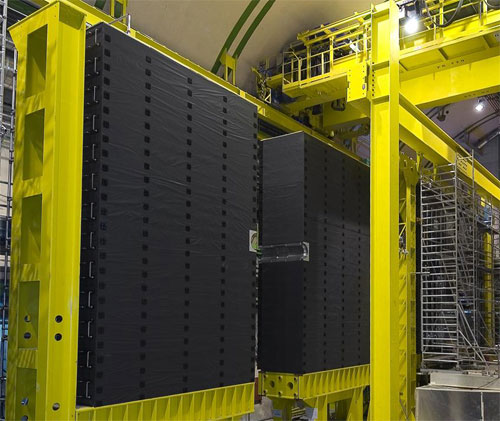
\includegraphics[height=3 cm]{Figures Introductory Lecture/LHCb Detector/LHCb_HCAL.jpg}%source:https://www.lhc-facts.ch/index.php?page=lhcb dort wird als quelle cern genannt
        \end{figure}
    \end{minipage}
    \vspace{-0.5cm}
    \begin{figure}[h]
    \centering
    \begin{overpic}[width=0.8\textwidth]{Figures Introductory Lecture/LHCb Detector/LHCb_8.png}
        \put (63.5,52) {\colorbox{LHCbDarkBlue!80}{\textcolor{LHCbLightBlue} {\centering \tiny  HCAL}}}
        \put (55,52) {\colorbox{lightgray}{\centering \tiny  ECAL}}
        \put (45.3,52) {\colorbox{lightgray}{\centering \tiny  RICH 2}}
        \put (42,46) {\rotatebox[]{90}{\colorbox{lightgray}{\centering \tiny  T1-T3}}}
        \put (27,52) {\colorbox{lightgray}{\centering \tiny  Magnet}}
        \put (20,40) {\rotatebox[]{90}{\colorbox{lightgray}{\centering \tiny  TT}}}
        \put (13,45) {\colorbox{lightgray}{\centering \tiny  RICH 1}}
        \put (3,35) {\colorbox{lightgray}{\centering \tiny  VELO}}

\put (1,5) {\tiny $z/m \rightarrow$}
\put (17.5,2) {\tiny $2$}
\put (21.4,2) {\tiny $3$}
\put (25.5,2) {\tiny $4$}

\put (39,2) {\tiny $7$}

\put (50,2) {\tiny $10$}
\put (57,2) {\tiny $12$}
\put (65,2) {\tiny $14$}

    \end{overpic}
    \end{figure}
\end{frame}
\begin{frame}
     \begin{figure}[h]
        \centering
        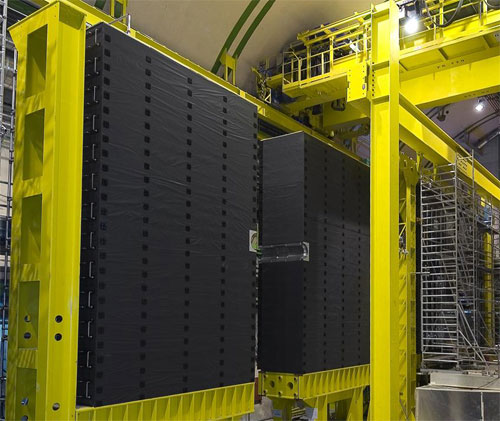
\includegraphics[height=\textheight]{Figures Introductory Lecture/LHCb Detector/LHCb_HCAL.jpg}%source:https://www.lhc-facts.ch/index.php?page=lhcb dort wird als quelle cern genannt
        \end{figure}
\end{frame}
%%%%%%%%%%%%%%%%%%%%%%%%%%%%%%%%%%%%%%%%%%%%%%%%%%%%%%%%%%%%%%%%%%%%%%%%%%%%%%%%%%%%%%%%%%%%%%
\begin{frame}{Myonenkammern}
    \begin{minipage}{0.58\textwidth}
    \begin{itemize}
        \item Misst \textcolor{red}{\textbf{Position}} von Myonen
    \end{itemize}
    \end{minipage}\hfill
    \begin{minipage}{0.38\textwidth}
        \begin{figure}[h]
        \centering
        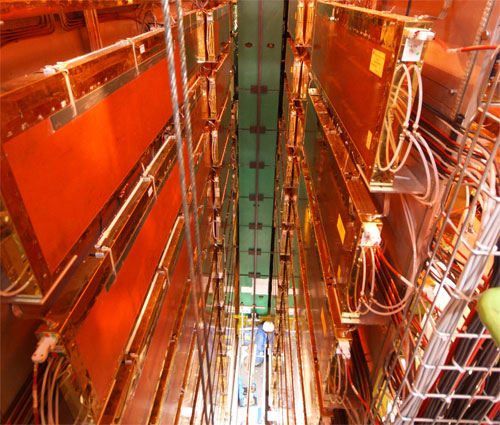
\includegraphics[height=3 cm]{Figures Introductory Lecture/LHCb Detector/LHCb_Muon.jpg}%source:https://www.lhc-facts.ch/index.php?page=lhcb dort wird als quelle cern genannt
        \end{figure}
    \end{minipage}
    \vspace{-0.5cm}
    \begin{figure}[h]
    \centering
    \begin{overpic}[width=0.8\textwidth]{Figures Introductory Lecture/LHCb Detector/LHCb_9.png}
        \put (85,50) {\colorbox{LHCbDarkBlue!80}{\textcolor{LHCbLightBlue}{\parbox{1.25cm}{\centering \tiny  Myonen Kammern}}}}
        \put (63.5,52) {\colorbox{lightgray}{\centering \tiny  HCAL}}
        \put (55,52) {\colorbox{lightgray}{\centering \tiny  ECAL}}
        \put (45.3,52) {\colorbox{lightgray}{\centering \tiny  RICH 2}}
        \put (42,46) {\rotatebox[]{90}{\colorbox{lightgray}{\centering \tiny  T1-T3}}}
        \put (27,52) {\colorbox{lightgray}{\centering \tiny  Magnet}}
        \put (20,40) {\rotatebox[]{90}{\colorbox{lightgray}{\centering \tiny  TT}}}
        \put (13,45) {\colorbox{lightgray}{\centering \tiny  RICH 1}}
        \put (7,52) {\colorbox{lightgray}{\centering \tiny  VELO}}

\put (1,5) {\tiny $z/m \rightarrow$}
\put (17.5,2) {\tiny $2$}
\put (21.4,2) {\tiny $3$}
\put (25.5,2) {\tiny $4$}

\put (39,2) {\tiny $7$}

\put (50,2) {\tiny $10$}
\put (57,2) {\tiny $12$}
\put (65,2) {\tiny $14$}
\put (73.5,2) {\tiny $16$}
\put (86,2) {\tiny $20$}
    \end{overpic}
    \end{figure}
\end{frame}
\begin{frame}
     \begin{figure}[h]
        \centering
        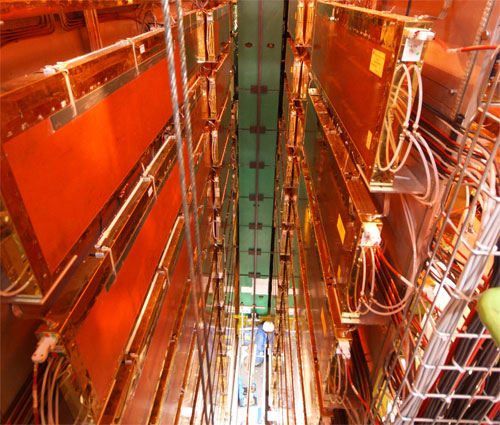
\includegraphics[height=\textheight]{Figures Introductory Lecture/LHCb Detector/LHCb_Muon.jpg}%source:https://www.lhc-facts.ch/index.php?page=lhcb dort wird als quelle cern genannt
        \end{figure}
\end{frame}
%%%%%%%%%%%%%%%%%%%%%%%%%%%%%%%%%%%%%%%%%%%%%%%%%%%%%%%%%%%%%%%%%%%%%%%%%%%%%%%%%%%%%%%%%%%%%%
\subsection{}
\begin{frame}{Messbereich von LHCb}
\begin{figure}[h]
    \centering
    \begin{overpic}[width=\textwidth]{Figures Introductory Lecture/LHCb Detector/LHCb_10.png}
        \put (85,50) {\colorbox{lightgray}{\parbox{1.25cm}{\centering \tiny  Myonen Kammern}}}
        \put (63.5,52) {\colorbox{lightgray}{\centering \tiny  HCAL}}
        \put (55,52) {\colorbox{lightgray}{\centering \tiny  ECAL}}
        \put (45.3,52) {\colorbox{lightgray}{\centering \tiny  RICH 2}}
        \put (42,46) {\rotatebox[]{90}{\colorbox{lightgray}{\centering \tiny  T1-T3}}}
        \put (27,52) {\colorbox{lightgray}{\centering \tiny  Magnet}}
        \put (20,40) {\rotatebox[]{90}{\colorbox{lightgray}{\centering \tiny  TT}}}
        \put (13,45) {\colorbox{lightgray}{\centering \tiny  RICH 1}}
        \put (3,35) {\colorbox{lightgray}{\centering \tiny  VELO}}

\put (1,5) {\tiny $z/m \rightarrow$}
\put (5,56) {\tiny $y/m$}
\put (17.5,2) {\tiny $2$}
\put (21.4,2) {\tiny $3$}
\put (25.5,2) {\tiny $4$}

\put (39,2) {\tiny $7$}

\put (50,2) {\tiny $10$}
\put (57,2) {\tiny $12$}
\put (65,2) {\tiny $14$}
\put (73.5,2) {\tiny $16$}
\put (86,2) {\tiny $20$} 

\put (7,50.5) {\tiny $+5$} 
\put (6,30.5) {\tiny $0$} 
\put (7,9.5) {\tiny $-5$} 


    \end{overpic}
    \end{figure}
\end{frame}
\subsection{Bild: CERN}
\begin{frame}
    \includegraphics[width=\textwidth]{Figures Introductory Lecture/LHCb Detector/LHCb_image.jpg}
\end{frame}
\begin{frame}
    \begin{overpic}[width=\textwidth]{Figures Introductory Lecture/LHCb Detector/LHCb_image+scheme.jpg.png}
            \put(78,50){\colorbox{lightgray}{\tiny  VELO}}
            \put(73.5,50){\colorbox{lightgray}{\rotatebox[]{90}{\tiny RICH 1}}}
            \put(70.5,50){\colorbox{lightgray}{\rotatebox[]{90}{\tiny TT}}}
            \put(57,60){\colorbox{lightgray}{\tiny Magnet}}
            \put(49,50){\colorbox{lightgray}{\rotatebox[]{90}{\tiny T1-T3}}}
            \put(41,60){\colorbox{lightgray}{\tiny RICH 2}}
            \put(32,60){\colorbox{lightgray}{\tiny ECAL}}
            \put(25,60){\colorbox{lightgray}{\tiny HCAL}}
            \put(11,60){\colorbox{lightgray}{\parbox{1.25cm}{\tiny Myonen Kammern}}}
                    
    \end{overpic}
\end{frame}
\subsection{}
% \begin{frame}{Was macht wo ein Signal?}
% \begin{figure}[h]
%     \centering
%     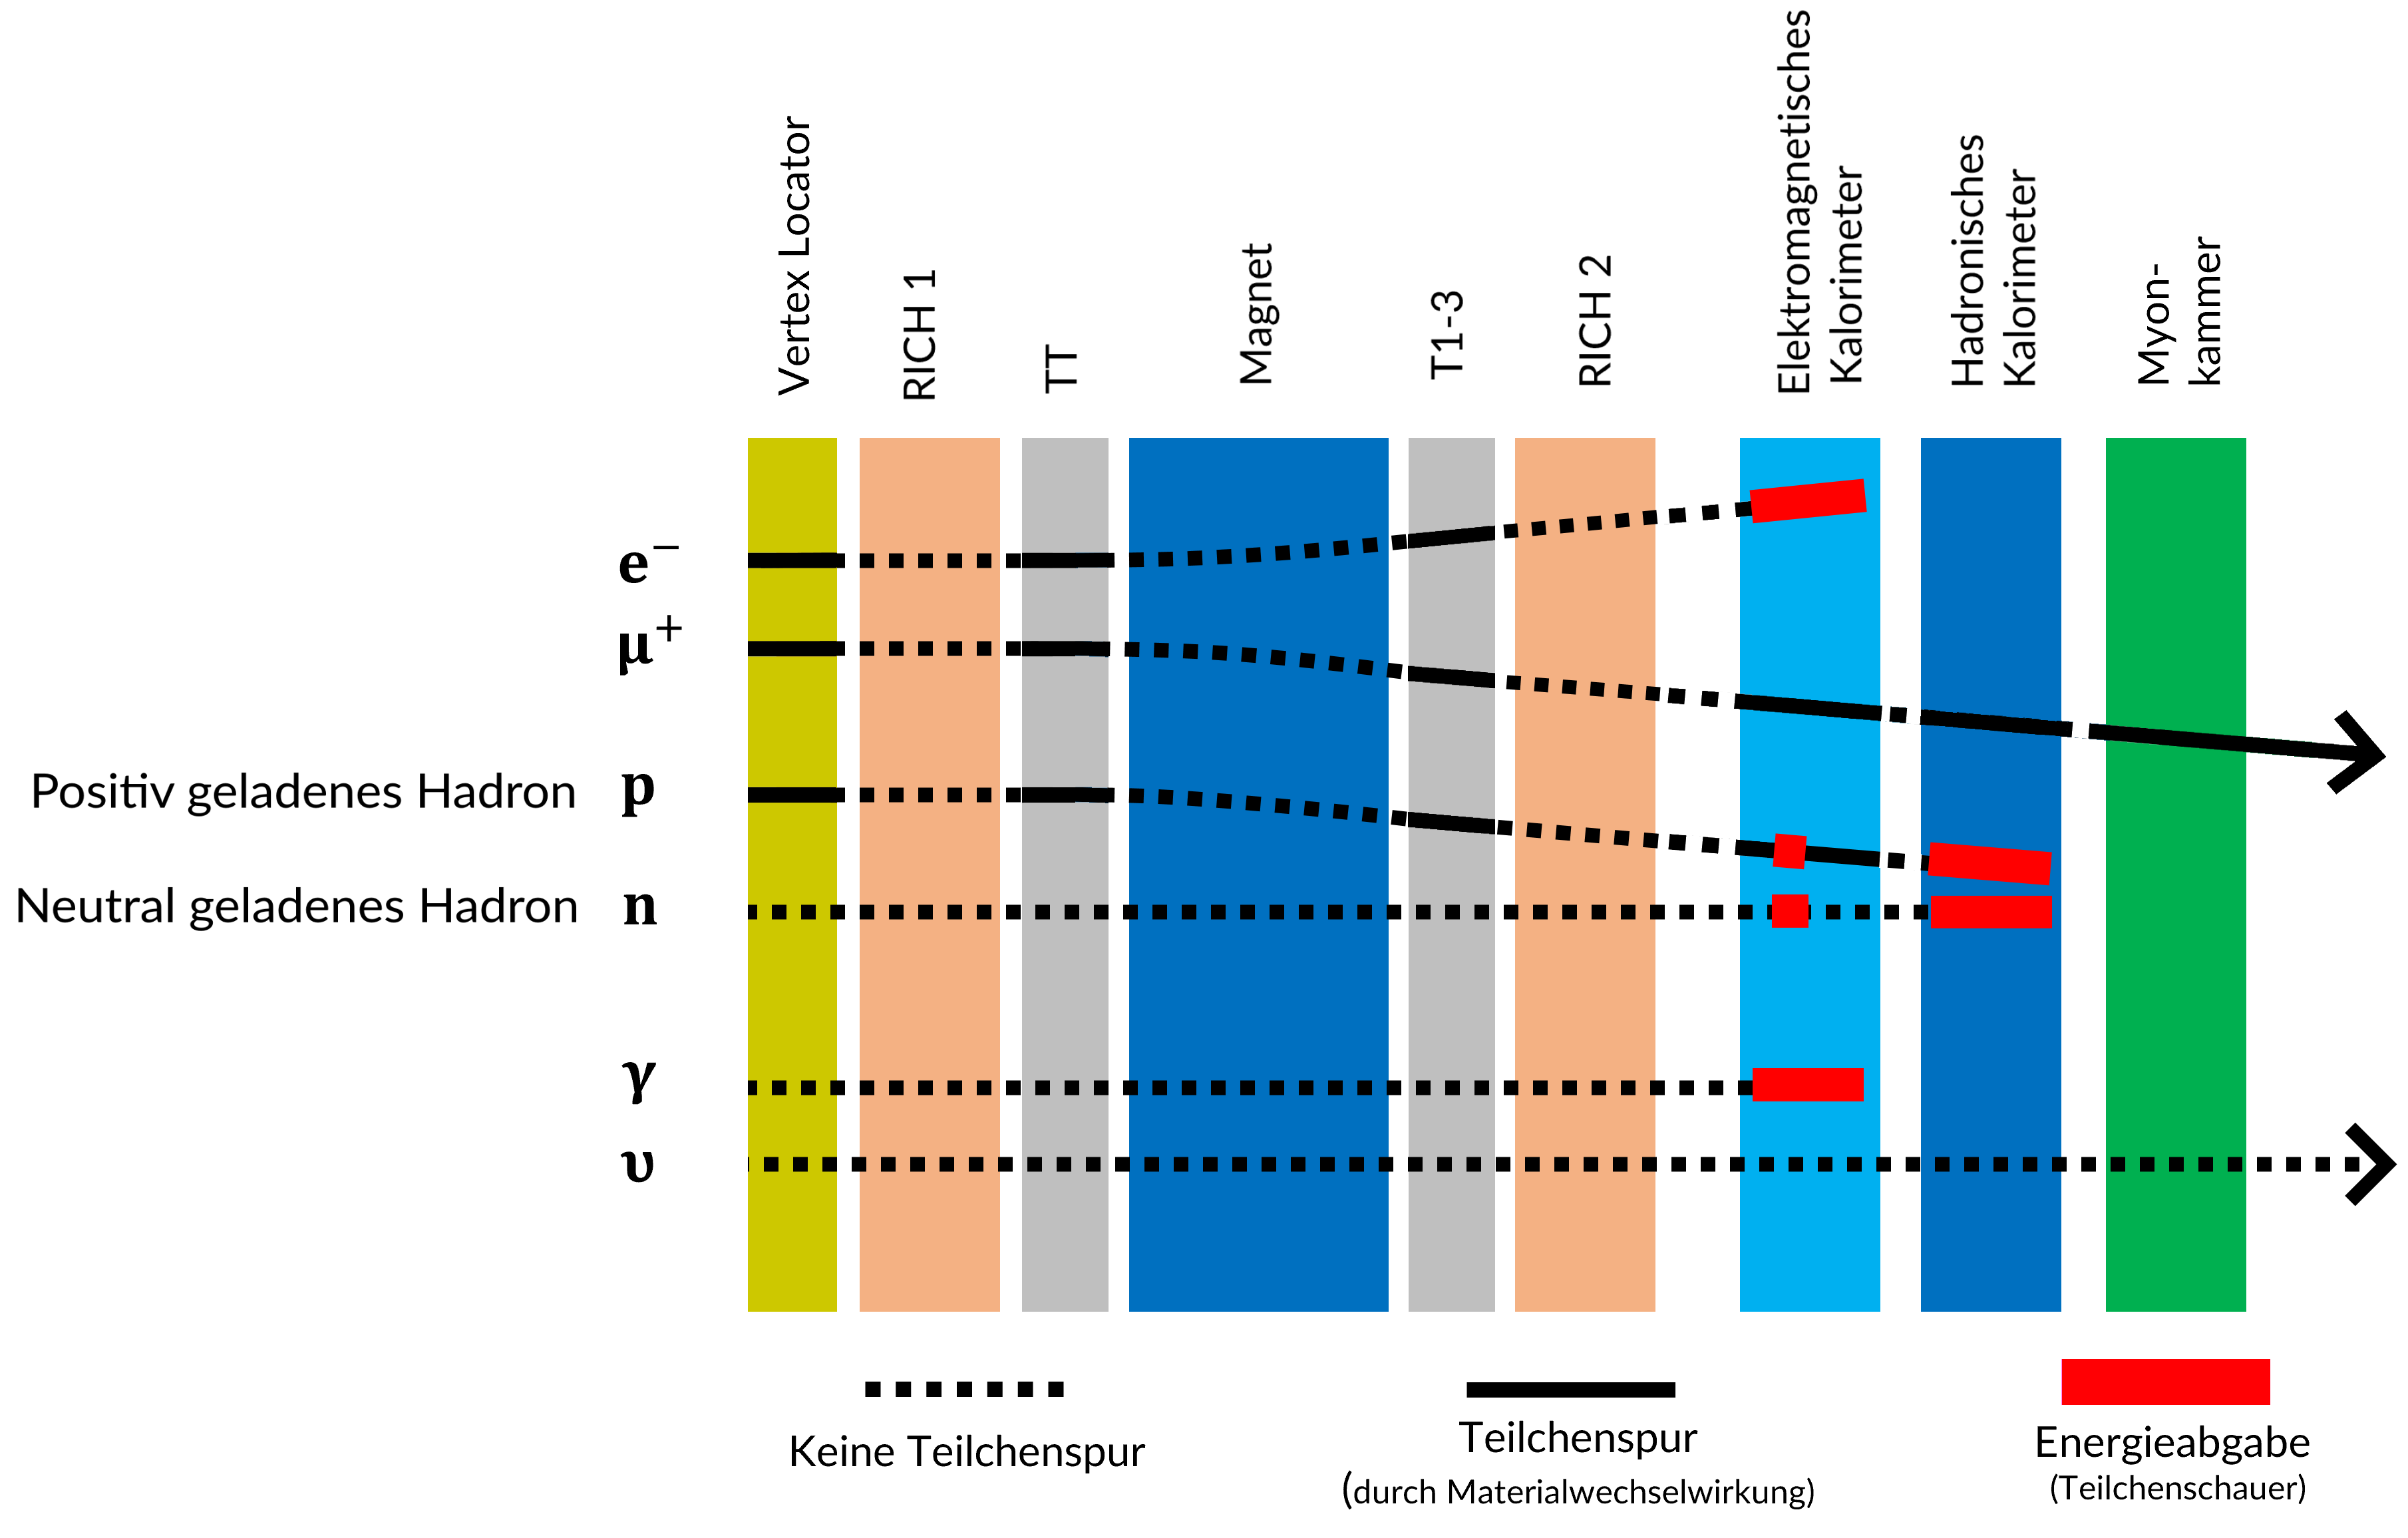
\includegraphics[width=\textwidth]{Figures Introductory Lecture/LHCb Detector/Energy Depostition LHCb.png}
%     %\c%aption{%Caption}
%     \label{fig:energy_deposition}
% \end{figure}
% \end{frame}

\begin{frame}{Was macht wo ein Signal?}
\vspace{-1cm}
\begin{center}
        \begin{tikzpicture}
%Boxen
        \draw[fill=VELO!80, line width=0.01] (0,0)--(0.5,0)--(0.5,5)  to node [black, above]{\rotatebox{90}{\scriptsize VELO}} (0,5) -- (0,0) ;
        \draw[fill=RICH, line width=0.01] (0.7,0)--(1.7,0)--(1.7,5) to node [black, above]{\rotatebox{90}{\scriptsize RICH 1}} (0.7,5)--(0.7,0);
           \draw[fill=gray,line width=0] (1.9,0)--(2.4,0)--(2.4,5) to node [black, above]{\rotatebox{90}{\scriptsize TT}} (1.9,5)-- (1.9,0);
        \draw[fill=Magnet,line width=0] (2.6,0)--(4.3,0)--(4.3,5) to node [black, above]{\rotatebox{90}{\scriptsize Magnet}} (2.6,5)-- (2.6,0);
        \draw[fill=gray,line width=0] (4.5,0)--(5,0)--(5,5)to node [black, above]{\rotatebox{90}{\scriptsize T1-T3}}(4.5,5)-- (4.5,0);
        \draw[fill=RICH,line width=0] (5.2,0)--(6.2,0)--(6.2,5)to node [black, above]{\rotatebox{90}{\scriptsize RICH 2}}(5.2,5)-- (5.2,0);
        \draw[fill=ECAL,line width=0] (6.4,0)--(7.4,0)--(7.4,5)to node [black, above]{\rotatebox{90}{\scriptsize ECAL}}(6.4,5)-- (6.4,0);
        \draw[fill=HCAL,line width=0] (7.6,0)--(8.6,0)--(8.6,5)to node [black, above]{\rotatebox{90}{\parbox{2cm}{\scriptsize HCAL}}}(7.6,5)-- (7.6,0);
                \draw[fill=Muon,line width=0] (8.8,0)--(9.8,0)--(9.8,5)to node [black, above]{\rotatebox{90}{\parbox{1.5cm}{\scriptsize Myonen Kammern}}}(8.8,5)-- (8.8,0);

%Elektron
        \draw[--, black, line width=0.5mm](-0.5,4) to node[black,left=5pt]{$e^-$} (0,4) to (0.5,4)  (1.9,4) to (2.4,4) (4.5,4.24) to (5,4.32){};
        \draw[--, black, dotted, line width=0.5mm] (0.5,4) to (1.9,4) (2.4,4) to (2.6,4) to [out=0,in=200,bend right=5] (4.3, 4.2) to (4.5,4.24) (5,4.32) to (6.9,4.62);
        \draw[--, red,  line width=2mm,cap=round]  (6.6,4.57) to  (7.2,4.67);

%Antimyon
        \draw[--, black, line width=0.5mm](-0.5,3.5) to node[black,left=5pt]{$\mu^+$} (0,3.5) to (0.5,3.5)  (1.9,3.5) to (2.4,3.5) (4.5,3.26) to (5,3.18)  (6.4,2.9) to (7.4,2.7)(7.6,2.66) to (8.6,2.46) (8.8,2.42) to (9.8,2.22){};
        \draw[--, black, dotted, line width=0.5mm] (0.5,3.5) to (1.9,3.5) (2.4,3.5) to (2.6,3.5) to [out=0,in=200,bend left=5] (4.3, 3.3) to (4.5,3.26) (5,3.18) to (5.2,3.14) to (6.2,2.94) (6.2,2.94) to (6.4,2.9)(7.4,2.7) to (7.6,2.66)(8.6,2.46) to (8.8,2.42);
        \draw[-{Latex[length=3mm]},black,dotted, line width=0.5mm] (9.8,2.22) to (10.3,2.12){};

%Proton
        \draw[--, black, line width=0.5mm](-0.5,3) to node[black,left=10pt]{$p$} (0,3) to (0.5,3)  (1.9,3) to (2.4,3) (4.5,2.76) to (5,2.68)  (6.4,2.4) to (7.4,2.2)(7.6,2.16) (7.6,2.16) to (8.1,2.06){};
        \draw[--, black, dotted, line width=0.5mm] (0.5,3) to (1.9,3) (2.4,3) to (2.6,3) to [out=0,in=200,bend left=5] (4.3, 2.8) to (4.5,2.76) (5,2.68) to (5.2,2.64) to (6.2,2.44) (6.2,2.44) to (6.4,2.4)(7.4,2.2) to (7.6,2.16);
        \draw[--, red,  line width=2mm,cap=round]  (6.8,2.32) to  (7,2.28) (7.8,2.12) -- (8.4,1.98);



%Neutron
        \draw[--, black, dotted, line width=0.5mm](-0.5,1.75) to node[black,left=10pt]{$n$} (0,1.75)  to  (7.6,1.75) {};
        \draw[--, black, line width=0.5mm] (7.6,1.75) to (8.1,1.75) ;
         \draw[--, red,  line width=2mm,cap=round]  (6.8,1.75) to  (7,1.75) (7.8,1.75) -- (8.4,1.75);

%Photon
         \draw[--, black, dotted, line width=0.5mm](-0.5,1.25)  to node[black,left=10pt]{$\gamma$} (0,1.25) to (7.1,1.25) {};
         \draw[--, red,  line width=2mm,cap=round]  (6.6,1.25) to  (7.2,1.25){}; 


%Neutrino
        \draw[-{Latex[length=3mm]}, black,dotted, line width=0.5mm](-0.5,0.75) to node[black,left=10pt]{$\nu$} (0,0.75)  to (10.3,0.75) {};

%Legende
\draw[--, black, dotted, line width=0.5mm](0.5,-0.5) to  node[below, ] {\parbox{2.8cm}{\scriptsize Keine Teilchenspur}} (2.5,-0.5) ;\draw[--, black, line width=0.5mm] (3.5,-0.5) to  node[below, ] {\parbox{2cm}{\scriptsize Teilchenspur\\ \tiny (durch Materialwechelwirkung) }} (5.5,-0.5) ;\draw[--, red,  line width=2mm] (6.5,-0.5) to node[below, black ] {\parbox{2.3cm}{\scriptsize Energieabgabe\\ \tiny (Teilchenschauer)} } (8.5,-0.5) ;

    \end{tikzpicture}
    \end{center}
\end{frame}
%%%%%%%%%%%%%%%%%%%%%%%%%%%%%%%%%%%%%%%%%%%%%%%%%%%%%%%%%%%%%%%%%%%%%%%%%%%%%%%%%%%%%%%%%%%%%%
\begin{frame}{Wie sieht ein gemessenes Ereignis aus?}
\begin{figure}[h]
    \centering
    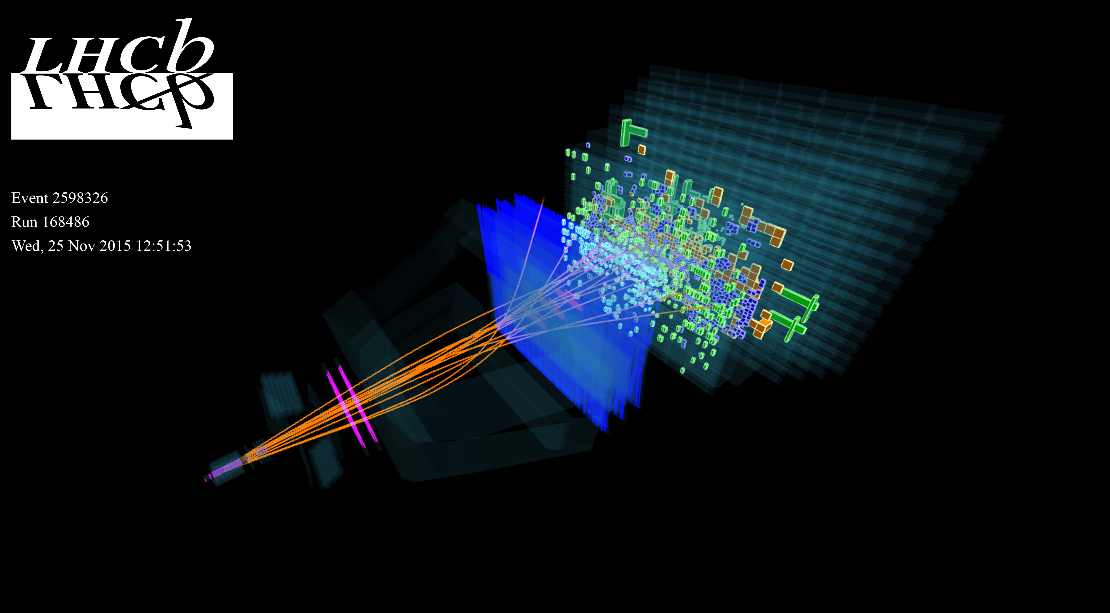
\includegraphics[width=\textwidth]{Figures Introductory Lecture/LHCb Detector/LHCb_Eventdisplay.png}
    %\c%aption{%Caption}
    \label{fig:energy_deposition}
\end{figure}
\end{frame}

%%%%%%%%%%%%%%%%%%%%%%%%%%%%%%%%%%%%%%%%%%%%%%%%%%%%%%%%%%%%%%%%%%%%%%%%%%%%%%%%%%%%%%%%%%%%%%
\newcommand\Bigbullet{\raisebox{-1.1mm}{\scalebox{2.5}{$\bullet$}}}
\newcommand\BigbulletG{\raisebox{-3mm}{\scalebox{5}{$\bullet$}}}

\begin{frame}
Additional slides \Bigbullet


\end{frame}

\begin{frame}{Quarkmassen}

    \begin{overpic}[width=1.05\textwidth]{Figures Introductory Lecture/Standard Model/SM_vis_1.png}%
        \put (3.3,15) {\small 2.2\,MeV/$c^2$}
    \end{overpic}
    
\end{frame}

\begin{frame}{Quarkmassen}

   \begin{overpic}[width=1.05\textwidth]{Figures Introductory Lecture/Standard Model/SM_vis_2.png}%
        \put (3.6,15) {\centering\footnotesize 2.2\,MeV/$c^2$}
          \put (6,20) {\centering\small 1\,kg}


    \end{overpic}
    
\end{frame}

\begin{frame}{Quarkmassen}

   \begin{overpic}[width=1.05\textwidth]{Figures Introductory Lecture/Standard Model/SM_vis_3.png}%
                \put (3.6,15) {\centering\footnotesize 2.2\,MeV/$c^2$}
          \put (6,20) {\centering\small 1\,kg}

          \put (18.6,15) {\centering\footnotesize 4.7\,MeV/$c^2$}
          \put (20,20) {\centering\small $\approx$ 2\,kg}



        

    \end{overpic}
    
\end{frame}
\subsection{Picture: schaette.de}
\begin{frame}{Quarkmassen}

   \begin{overpic}[width=1.05\textwidth]{Figures Introductory Lecture/Standard Model/SM_vis_4.png}%
                \put (3.6,15) {\centering\footnotesize 2.2\,MeV/$c^2$}
          \put (6,20) {\centering\small 1\,kg}

          \put (18.6,15) {\centering\footnotesize 4.7\,MeV/$c^2$}
          \put (20,20) {\centering\small $\approx$ 2\,kg}

          \put (32.6,15) {\centering\footnotesize 96\,MeV/$c^2$}
          \put (35,20) {\centering\small $\approx$ 45\,kg}

        

    \end{overpic}
    
\end{frame}
\subsection{Picture: schaette.de $|$ meinhaushalt.at}
\begin{frame}{Quarkmassen}

    \begin{overpic}[width=1.05\textwidth]{Figures Introductory Lecture/Standard Model/sm_vis_5.png}%
            \put (3.6,15) {\centering\footnotesize 2.2\,MeV/$c^2$}
          \put (6,20) {\centering\small 1\,kg}

          \put (18.6,15) {\centering\footnotesize 4.7\,MeV/$c^2$}
          \put (20,20) {\centering\small $\approx$ 2\,kg}

          \put (32.6,15) {\centering\footnotesize 96\,MeV/$c^2$}
          \put (35,20) {\centering\small $\approx$ 45\,kg}

        
         \put (48,15) {\centering\footnotesize 1.3\,GeV/$c^2$}
        \put (50,20) {\centering\small $\approx$ 0.6\,t}

   
    \end{overpic}
    
\end{frame}
\subsection{Picture: schaette.de $|$ meinhaushalt.at $|$ M 93 (2021)}
\begin{frame}{Quarkmassen}

   \begin{overpic}[width=1.05\textwidth]{Figures Introductory Lecture/Standard Model/SM_vis_6.png}%
        \put (3.6,15) {\centering\footnotesize 2.2\,MeV/$c^2$}
          \put (6,20) {\centering\small 1\,kg}

          \put (18.6,15) {\centering\footnotesize 4.7\,MeV/$c^2$}
          \put (20,20) {\centering\small $\approx$ 2\,kg}

          \put (32.6,15) {\centering\footnotesize 96\,MeV/$c^2$}
          \put (35,20) {\centering\small $\approx$ 45\,kg}

        
         \put (48,15) {\centering\footnotesize 1.3\,GeV/$c^2$}
        \put (50,20) {\centering\small $\approx$ 0.6\,t}

         \put (63,15) {\centering\footnotesize 4.2\,GeV/$c^2$}
          \put (64,20) {\centering\small $\approx$ 1.9\,t}
        
 
    \end{overpic}
    
\end{frame}
\subsection{Picture: schaette.de $|$  meinhaushalt.at $|$ M 93 (2021) $|$ Airbus}
\begin{frame}{Quarkmassen}

   \begin{overpic}[width=1.05\textwidth]{Figures Introductory Lecture/Standard Model/SM_vis_7.png}%
        \put (3.6,15) {\centering\footnotesize 2.2\,MeV/$c^2$}
          \put (6,20) {\centering\small 1\,kg}

          \put (18.6,15) {\centering\footnotesize 4.7\,MeV/$c^2$}
          \put (20,20) {\centering\small $\approx$ 2\,kg}

          \put (32.6,15) {\centering\footnotesize 96\,MeV/$c^2$}
          \put (35,20) {\centering\small $\approx$ 45\,kg}

        
         \put (48,15) {\centering\footnotesize 1.3\,GeV/$c^2$}
        \put (50,20) {\centering\small $\approx$ 0.6\,t}

         \put (63,15) {\centering\footnotesize 4.2\,GeV/$c^2$}
          \put (64,20) {\centering\small $\approx$ 1.9\,t}
        
        \put (77,15) {\centering\footnotesize 173\,GeV/$c^2$}
        \put (78,20) {\centering\small $\approx$ 79\,t}

    \end{overpic}
    
\end{frame}
\subsection{}
\begin{frame}
\begin{minipage} {0.3\textwidth}
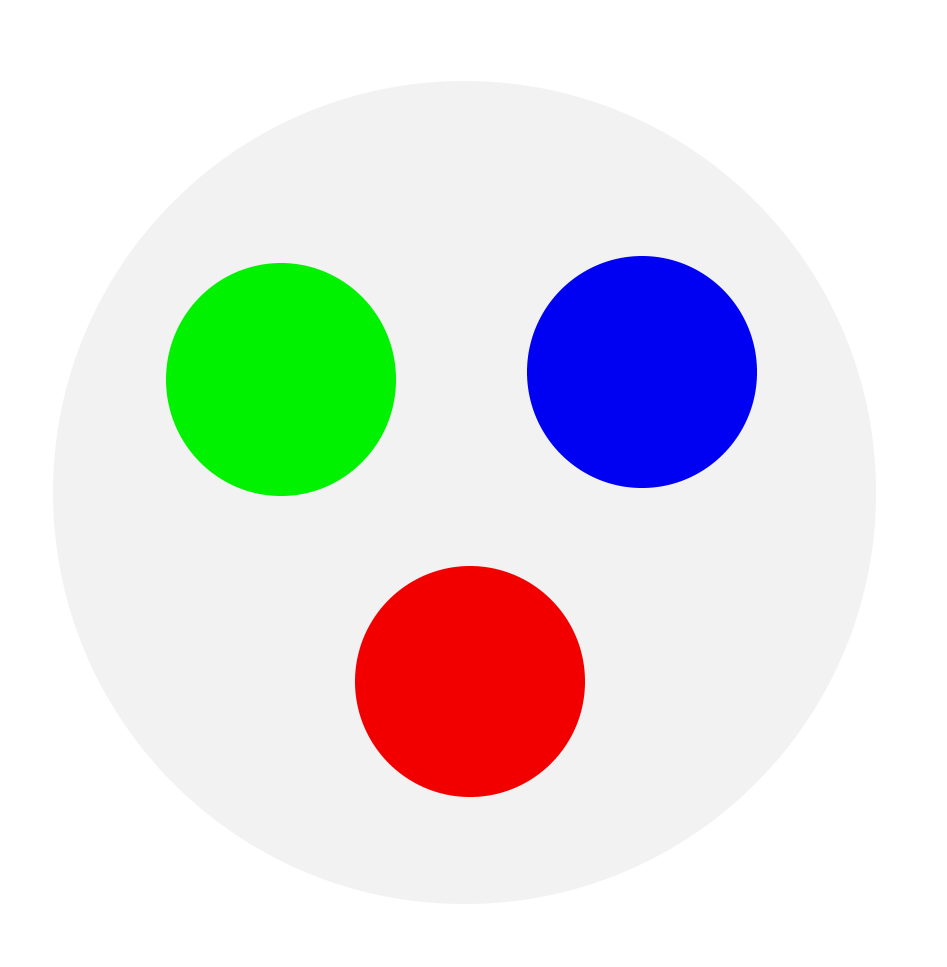
\includegraphics[width=\textwidth]{Figures Introductory Lecture/Standard Model/Hadron_coloured.png}
\end{minipage}
\begin{minipage} {0.65\textwidth}
Einfache Überlegung:\\  $m\big( \textcolor{lightgray}{ \BigbulletG}\big)\overset{?}{=}m(\textcolor{red}{\Bigbullet})+m(\textcolor{blue}{\Bigbullet})+m(\textcolor{green}{\Bigbullet})$
\end{minipage}
z.B. Proton ($uud$):\\
\begin{align*} 
m(u)&=2.2  \,\textmd{MeV}/c^2\\m(d)&= 4.7 \, \textmd{MeV}/c^2 \\ \rightarrow m(\textmd{Proton})&=9.1  \,\textmd{MeV}/c^2
\end{align*} 
Tatsächlich findet man:
\begin{align*} 
m(\textmd{Proton})=938  \,\textmd{MeV}/c^2
\end{align*} 
\end{frame}
\begin{frame}\addtocounter{framenumber}{-1}
\begin{minipage} {0.3\textwidth}
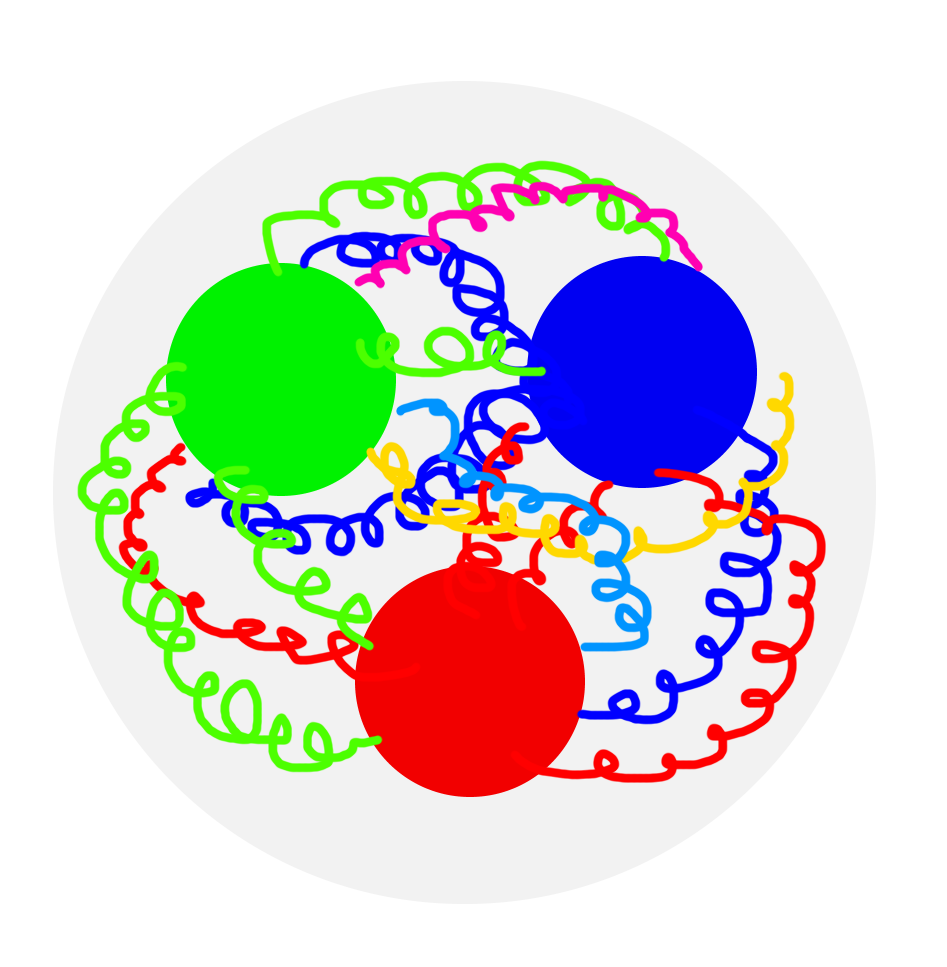
\includegraphics[width=\textwidth]{Figures Introductory Lecture/Standard Model/Hadron_seequarks_coloured.png}
\end{minipage}
\begin{minipage} {0.65\textwidth}
Einfache Überlegung:\\  $m\big( \textcolor{lightgray}{ \BigbulletG}\big)\neq m(\textcolor{red}{\Bigbullet})+m(\textcolor{blue}{\Bigbullet})+m(\textcolor{green}{\Bigbullet})$
\end{minipage}
z.B. Proton ($uud$):\\
\begin{align*} 
m(u)&=2.2  \,\textmd{MeV}/c^2\\m(d)&= 4.7 \, \textmd{MeV}/c^2 \\ \rightarrow m(\textmd{Proton})&=9.1  \,\textmd{MeV}/c^2
\end{align*} 
Tatsächlich findet man:
\begin{align*} 
m(\textmd{Proton})=938  \,\textmd{MeV}/c^2
\end{align*} 
\end{frame}
\begin{frame}{Referenzen}\scriptsize
\begin{itemize}
\item[-] Maximilien Brice/CERN (2018) \url{https://cds.cern.ch/images/CERN-PHOTO-201801-025-18/} 
\item[-] Maximilien Brice/CERN (2008). \url{cds.cern.ch/record/1295244}
\item[-] Paula Collins/CERN (2007)  \url{cds.cern.ch/record/1017398}
\item[-] Christoph Frei/CERN (2021)  \url{cds.cern.ch/record/2807064}
\item[-] Angela Buechler/CERN (2009)  \url{twiki.cern.ch/twiki/bin/view/LHCb/ConferenceSummaryIEEFlorida2009}
\item[-] Peter Ginter/CERN (2008) \url{cds.cern.ch/record/1124307}
\item[-] Maximilien Brice, Julien Ordan/CERN (2009)  \url{facebook.com/LHCbExperiment/photos/a.238680152959433/1123439814483458/?type=3}
\item[-] Maximilien Brice, Julien Ordan/CERN (2009)  \url{https://cds.cern.ch/record/2302374}
\item[-] CERN (2015). \url{https://lhcb.web.cern.ch/lhcb_page/collaboration/LHCb20/ }
\item[-] Maximilien Brice/CERN (2005)  \url{cds.cern.ch/record/835712}
\item[-] schaette.de. \url{schaette.de/ratgeber/tiergesundheit/rinder/rinder-was-koennen-wir-fuer-abwehrstarke-kaelber-tun}
\item[-] meinhaushalt.at (2009). \url{meinhaushalt.at/4182-zunge-schalen-kochen/#}
\item[-] M 93 (2021) BMW X3 xDrive20d xLine (G01) – h 02042021.jpg
\item[-] Airbus. \url{aircraft.airbus.com/en/aircraft/a320/a321xlr#images}

\end{itemize}
\end{frame}
\end{document}